% Judul dokumen
\title{Buku Tugas Akhir ITS}
\author{Solang, Dion Andreas}

% Pengaturan ukuran teks dan bentuk halaman dua sisi
\documentclass[12pt,twoside]{report}
\usepackage{itss}

% Atur variabel berikut sesuai namanya

% nama
\newcommand{\name}{Dion Andreas Solang}
\newcommand{\authorname}{Solang, Dion Andreas}
\newcommand{\nickname}{Dion}
\newcommand{\advisor}{Reza Fuad Rachmadi, S.T., M.T., Ph.D}
\newcommand{\coadvisor}{Dr. I Ketut Eddy Purnama, S.T., M.T.}
\newcommand{\examinerone}{Dr. Diah Puspito Wulandari, S.T., M.Sc.}
\newcommand{\examinertwo}{Dr. Surya Sumpeno, S.T., M.Sc.}
\newcommand{\examinerthree}{Prof. Dr. Ir. Yoyon K. Suprapto, M.Sc.}
\newcommand{\headofdepartment}{Dr. Supeno Mardi Susiki Nugroho, S.T., M.T}

% identitas
\newcommand{\nrp}{0721 19 4000 0039}
  %\textmd{NIP } \\
\newcommand{\advisornip}{19850403201212 1 001}
\newcommand{\coadvisornip}{19690730199512 1 001}
\newcommand{\examineronenip}{19801219200501 2 001}
\newcommand{\examinertwonip}{19690613199702 1 003}
\newcommand{\examinerthreenip}{19540925197803 1 001}
\newcommand{\headofdepartmentnip}{19700313199512 1 001}

% judul
\newcommand{\tatitle}{OPTIMISASI PENDETEKSIAN OBJEK KECIL YOLOv7 UNTUK MENDETEKSI OBJEK-OBJEK \emph{AIRBORNE}}
\newcommand{\engtatitle}{\emph{YOLOv7 SMALL OBJECT DETECTION OPTIMIZATION TO DETECT AIRBORNE OBJECTS}}

% tempat
\newcommand{\place}{Surabaya}

% jurusan
\newcommand{\studyprogram}{Teknik Komputer}
\newcommand{\engstudyprogram}{Computer Engineering}

% fakultas
\newcommand{\faculty}{Fakultas Teknologi Elektro dan Informatika Cerdas}
\newcommand{\engfaculty}{Faculty of Intelligent Electrical and Informatics Technology}

% singkatan fakultas
\newcommand{\facultyshort}{FTEIC}
\newcommand{\engfacultyshort}{ELECTICS}

% departemen
\newcommand{\department}{Teknik Komputer}
\newcommand{\engdepartment}{Computer Engineering}

% kode mata kuliah
\newcommand{\coursecode}{EC184801}


% Tambahkan format tanda hubung yang benar di sini
\hyphenation{
  ro-ket
  me-ngem-bang-kan
  per-hi-tu-ngan
  tek-no-lo-gi
  me-la-ku-kan
  ber-so-si-al-i-sa-si
}

% Menambahkan resource daftar pustaka
\addbibresource{misc/bibliography.bib}

% Isi keseluruhan dokumen
\begin{document}


% Sampul luar Bahasa Indonesia
\newcommand\covercontents{cover/cover-content-id.tex}
\AddToShipoutPictureBG*{
  \AtPageLowerLeft{
    % Ubah nilai berikut jika posisi horizontal background tidak sesuai
    \hspace{-3.25mm}

    % Ubah nilai berikut jika posisi vertikal background tidak sesuai
    \raisebox{0mm}{
      
\includegraphics[width=\paperwidth,height=\paperheight]{cover/background/cover-outer-1.png}
    }
  }
}

% Menyembunyikan nomor halaman
\thispagestyle{empty}

% Pengaturan margin untuk menyesuaikan konten sampul
\newgeometry{
  top=55mm,
  left=30mm,
  right=20mm,
  bottom=20mm
}

\begin{flushleft}

  % Pemilihan font sans serif
  \sffamily

  % Pemilihan warna font putih
  \color{white}

  % Pemilihan font bold
  \fontseries{bx}
  \selectfont
  \begin{spacing}{1.5}
    \input{\covercontents}
  \end{spacing}

\end{flushleft}

\restoregeometry

\cleardoublepage

% Atur ulang penomoran halaman
\setcounter{page}{1}

% cover dalam Bahasa Indonesia
\renewcommand\covercontents{cover/cover-content-id.tex}
\AddToShipoutPictureBG*{
  \AtPageLowerLeft{
    % Ubah nilai berikut jika posisi horizontal background tidak sesuai
    \hspace{-4mm}

    % Ubah nilai berikut jika posisi vertikal background tidak sesuai
    \raisebox{0mm}{
      
\includegraphics[width=\paperwidth,height=\paperheight]{cover/background/cover-outer-2.png}
    }
  }
}

% Menyembunyikan nomor halaman
\thispagestyle{empty}

% Pengaturan margin untuk menyesuaikan konten sampul
\newgeometry{
  top=65mm,
  left=30mm,
  right=30mm,
  bottom=20mm
}

\begin{flushleft}

  % Pemilihan font sans serif
  \sffamily

  % Pemilihan font bold
  \fontseries{bx}
  \selectfont
  \begin{spacing}{1.5}
    \input{\covercontents}
  \end{spacing}

\end{flushleft}

\restoregeometry

\clearpage
\cleardoublepage

% cover dalam Bahasa Inggris
\renewcommand\covercontents{cover/cover-content-en.tex}
\AddToShipoutPictureBG*{
  \AtPageLowerLeft{
    % Ubah nilai berikut jika posisi horizontal background tidak sesuai
    \hspace{-4mm}

    % Ubah nilai berikut jika posisi vertikal background tidak sesuai
    \raisebox{0mm}{
      
\includegraphics[width=\paperwidth,height=\paperheight]{cover/background/cover-outer-2.png}
    }
  }
}

% Menyembunyikan nomor halaman
\thispagestyle{empty}

% Pengaturan margin untuk menyesuaikan konten sampul
\newgeometry{
  top=65mm,
  left=30mm,
  right=30mm,
  bottom=20mm
}

\begin{flushleft}

  % Pemilihan font sans serif
  \sffamily

  % Pemilihan font bold
  \fontseries{bx}
  \selectfont
  \begin{spacing}{1.5}
    \input{\covercontents}
  \end{spacing}

\end{flushleft}

\restoregeometry

\cleardoublepage


%% Lembar pengesahan
%\addcontentsline{toc}{chapter}{LEMBAR PENGESAHAN}
\begin{center}
	\large
  \textbf{LEMBAR PENGESAHAN}
\end{center}

% Menyembunyikan nomor halaman
\thispagestyle{empty}

\begin{center}
  % Ubah kalimat berikut dengan judul tugas akhir
  %\textbf{KALKULASI ENERGI PADA ROKET LUAR ANGKASA BERBASIS \emph{ANTI-GRAVITASI}}
  \textbf{OPTIMISASI PENDETEKSIAN OBJEK KECIL YOLOv7 UNTUK MENDETEKSI OBJEK-OBJEK \emph{AIRBORNE}}
\end{center}

\begingroup
  % Pemilihan font ukuran small
  \small

  \begin{center}
    % Ubah kalimat berikut dengan pernyataan untuk lembar pengesahan
    \textbf{PROPOSAL TUGAS AKHIR} \\
    Diajukan untuk memenuhi salah satu syarat \\
    memperoleh gelar Sarjana Teknik pada \\
    Program Studi S-1 Teknik Komputer \\
    Departemen Teknik Komputer \\
    Fakultas Teknologi Elektro dan Informatika Cerdas \\
    Institut Teknologi Sepuluh Nopember
  \end{center}

  \vspace{4ex}

  \begin{center}
    % Ubah kalimat berikut dengan nama dan NRP mahasiswa
    Oleh: \textbf{Dion Andreas Solang} \\
    NRP. 0721 19 4000 0039
  \end{center}

  \vspace{4ex}

  \begin{center}
    Disetujui oleh Tim Penguji Proposal Tugas Akhir:
  \end{center}

  \begingroup
    % Menghilangkan padding
    \setlength{\tabcolsep}{0pt}

    \noindent
    \begin{tabularx}{\textwidth}{X c}
      % Ubah kalimat-kalimat berikut dengan nama dan NIP dosen pembimbing pertama
      Reza Fuad Rachmadi, S.T., M.T., Ph.D          & (Pembimbing) \\
      NIP: 19850403201212 1 001      & \\
      &  \\
      &  \\
      % Ubah kalimat-kalimat berikut dengan nama dan NIP dosen pembimbing kedua
      Dr. I Ketut Eddy Purnama S.T., M.T.    & (Ko-Pembimbing) \\
      NIP: 19690730199512 1 001        & \\
      &  \\
      &  \\
      % Ubah kalimat-kalimat berikut dengan nama dan NIP dosen penguji pertama
      TBA  & (Penguji I) \\
      NIP: TBA        & \\
      &  \\
      &  \\
      % Ubah kalimat-kalimat berikut dengan nama dan NIP dosen penguji kedua
      TBA  & (Penguji II) \\
      NIP: TBA        & \\
      &  \\
      &  \\
      % Ubah kalimat-kalimat berikut dengan nama dan NIP dosen penguji ketiga
      TBA             & (Penguji III) \\
      NIP: TBA        & \\
    \end{tabularx}
  \endgroup

  \vspace{8ex}

  \begin{center}
    % Ubah text dibawah menjadi tempat dan tanggal
    \textbf{SURABAYA} \\
    \textbf{Februari, 2023}
  \end{center}
\endgroup

%\cleardoublepage
%\begin{center}
	\large
  \textbf{APPROVAL SHEET}
\end{center}

% Menyembunyikan nomor halaman
\thispagestyle{empty}

\begin{center}
  % Ubah kalimat berikut dengan judul tugas akhir
  \textbf{\emph{ANTI-GRAVITY} BASED ENERGY CALCULATION ON OUTER SPACE ROCKETS}
\end{center}

\begingroup
  % Pemilihan font ukuran small
  \small

  \begin{center}
    % Ubah kalimat berikut dengan pernyataan untuk lembar pengesahan
    \textbf{FINAL PROJECT PROPOSAL} \\
    Submitted to fulfill one of the requirements for obtaining a degree
    Bachelor of Engineering at 
    Undergraduate Study Program of Aerospace Engineering \\
    Department of Aerospace Engineering \\
    Faculty of Aerospace Technology \\
    Sepuluh Nopember Institute of Technology
  \end{center}

  \begin{center}
    % Ubah kalimat berikut dengan nama dan NRP mahasiswa
    By: \textbf{Elon Reeve Musk} \\
    NRP. 0123 20 4000 0001
  \end{center}

  \begin{center}
    Approved by Final Project Proposal Examiner Team:
  \end{center}

  \begingroup
    % Menghilangkan padding
    \setlength{\tabcolsep}{0pt}

    \noindent
    \begin{tabularx}{\textwidth}{X c}
      % Ubah kalimat-kalimat berikut dengan nama dan NIP dosen pembimbing pertama
      Nikola Tesla, S.T., M.T.          & (Advisor) \\
      NIP: 18560710 194301 1 001        & \\
      &  \\
      &  \\
      % Ubah kalimat-kalimat berikut dengan nama dan NIP dosen pembimbing kedua
      Wernher von Braun, S.T., M.T.     & (Co-Advisor) \\
      NIP: 19230323 197706 1 001        & \\
      &  \\
      &  \\
      % Ubah kalimat-kalimat berikut dengan nama dan NIP dosen penguji pertama
      Dr. Galileo Galilei, S.T., M.Sc.  & (Examiner I) \\
      NIP: 15640215 164201 1 001        & \\
      &  \\
      &  \\
      % Ubah kalimat-kalimat berikut dengan nama dan NIP dosen penguji kedua
      Friedrich Nietzsche, S.T., M.Sc.  & (Examiner II) \\
      NIP: 18441015 190008 1 001        & \\
      &  \\
      &  \\
      % Ubah kalimat-kalimat berikut dengan nama dan NIP dosen penguji ketiga
      Alan Turing, ST., MT.             & (Examiner III) \\
      NIP: 19120623 195406 1 001        & \\
    \end{tabularx}
  \endgroup

  \vspace{4ex}

  \begin{center}
    % Ubah text dibawah menjadi tempat dan tanggal
    \textbf{SURABAYA} \\
    \textbf{May, 2077}
  \end{center}
\endgroup

%\cleardoublepage
%
%% Pernyataan keaslian
%\begin{center}
  \large
  \textbf{PERNYATAAN ORISINALITAS}
\end{center}

% Menyembunyikan nomor halaman
\thispagestyle{empty}

\vspace{2ex}

% Ubah paragraf-paragraf berikut sesuai dengan yang ingin diisi pada pernyataan keaslian

\noindent Yang bertanda tangan dibawah ini:

\noindent\begin{tabularx}{\textwidth}{l l X}
                         &   &                            \\
  Nama Mahasiswa / NRP   & : & \name{} / \nrp{}           \\
  Departemen             & : & \department{}              \\
  Dosen Pembimbing / NIP & : & \advisor{} / \advisornip{} \\
                         &   &                            \\
\end{tabularx}

Dengan ini menyatakan bahwa Tugas Akhir dengan judul "\tatitle{}" adalah hasil karya sendiri, berfsifat orisinal, dan ditulis dengan mengikuti kaidah penulisan ilmiah.

Bilamana di kemudian hari ditemukan ketidaksesuaian dengan pernyataan ini, maka saya bersedia menerima sanksi sesuai dengan ketentuan yang berlaku di Institut Teknologi Sepuluh Nopember.

\vspace{8ex}

\noindent\begin{tabularx}{\textwidth}{X l}
                     & \place{}, \ENGMONTH{} \the\year{} \\
                     &                                   \\
  Mengetahui         &                                   \\
  Dosen Pembimbing   & Mahasiswa                         \\
                     &                                   \\
                     &                                   \\
                     &                                   \\
                     &                                   \\
                     &                                   \\
  \advisor{}         & \name{}                           \\
  NIP. \advisornip{} & NRP. \nrp{}                       \\
\end{tabularx}

%\cleardoublepage
%\begin{center}
  \large
  \textbf{STATEMENT OF ORIGINALITY}
\end{center}

% Menyembunyikan nomor halaman
\thispagestyle{empty}

\vspace{2ex}

% Ubah paragraf-paragraf berikut sesuai dengan yang ingin diisi pada pernyataan keaslian

\noindent The undersigned below:

\noindent\begin{tabularx}{\textwidth}{l l X}
                        &   &                            \\
  Name of student / NRP & : & \name{} / \nrp{}           \\
  Department            & : & \engdepartment{}           \\
  Advisor / NIP         & : & \advisor{} / \advisornip{} \\
                        &   &                            \\
\end{tabularx}

Hereby declared that the Final Project with the title of "\engtatitle{}" is the result of my own work, is original, and is written by following the rules of scientific writing.

If in future there is a discrepancy with this statement, then I am willing to accept sanctions in accordance with provisions that apply at Sepuluh Nopember Institute of Technology.

\vspace{8ex}

\noindent\begin{tabularx}{\textwidth}{X l}
                     & \place{}, \ENGMONTH{} \the\year{} \\
                     &                                   \\
  Acknowledged       &                                   \\
  Advisor            & Student                           \\
                     &                                   \\
                     &                                   \\
                     &                                   \\
                     &                                   \\
                     &                                   \\
  \advisor{}         & \name{}                           \\
  NIP. \advisornip{} & NRP. \nrp{}                       \\
\end{tabularx}
%\cleardoublepage

% Nomor halaman pembuka dimulai dari sini
\pagenumbering{roman}

% Abstrak Bahasa Indonesia
\begin{center}
  \large\textbf{ABSTRAK}
\end{center}

\addcontentsline{toc}{chapter}{ABSTRAK}

\vspace{2ex}

\begingroup
% Menghilangkan padding
\setlength{\tabcolsep}{0pt}

\noindent
\begin{tabularx}{\textwidth}{l >{\centering}m{2em} X}
  Nama Mahasiswa    & : & \name{}         \\

  Judul Tugas Akhir & : & \tatitle{}      \\

  Pembimbing        & : & 1. \advisor{}   \\
                    &   & 2. \coadvisor{} \\
\end{tabularx}
\endgroup

% Ubah paragraf berikut dengan abstrak dari tugas akhir
%Pada penelitian ini kami mengajukan \lipsum[1]
%Pada penelitian ini, kami menunjukan percobaan kami untuk meningkatkan kapabilitas YOLOv7
%untuk mendeteksi objek airborne. Objek airborne tampak sangat kecil pada kamera karena
%jarak yang cukup jauh dari kamera. Oleh karena itu, YOLOv7 harus dioptimisasi untuk
%dapat mendeteksi objek-objek kecil. Beberapa modifikasi diajukan dan diuji pada penelitian
%ini. Modifikasi-modifikasi ini meliput perubahan arsitektur (Menambah layer deteksi, mengubah
%sumber feature-map, dan mengganti layer deteksi menjadi anchor-free), dan pada bag-of-freebies
%(rekalkulasi anchor, dan augmentasi mosaik). Hingga saat ini, kami menemukan bahwa kombinasi
%augmentasi mosaik, rekalkulasi anchor, dan mengubah sumber feature-map memberikan skor
%mAP yang paling tinggi 14,09\% dibandingkan dengan YOLOv7 yang biasa (mAP=0\%).

%Pada penelitian ini, kami menunjukan percobaan kami untk meningkatkan kapabilitas dari YOLOv7 untuk mendeteksi objek airborne.
%Objek airborne tampak 
Pada penelitian ini, kami menunjukan percobaan kami untuk meningkatkan kemampuan deteksi YOLOv7 terhadap objek \emph{airborne}. 
Objek-objek di \emph{airborne} tampak sangat kecil pada gambar kamera ketika berada dalam jarak yang jauh. Namun, karena kecepatan pergerakan objek \emph{airborne} itu tinggi, penting untuk mendeteksinya saat masih berada dalam jarak yang jauh. 
Oleh karena itu, YOLOv7 perlu dioptimalkan untuk dapat mendeteksi objek-objek kecil dengan baik. 
Dalam penelitian ini, kami mengusulkan beberapa modifikasi yang berupa perubahan dalam arsitektur (menambahkan kepala deteksi tambahan, mengalihkan skala fitur deteksi, dan mengganti \emph{head} YOLO dengan \emph{decoupled anchor-free head}), penerapan teknik \emph{bag-of-freebies} (rekalkulasi anchor dan augmentasi mosaik), serta merubah proses inferensi (mempartisi gambar dan melakukan inferensi pada setiap partisi). 
Melalui eksperimen yang komprehensif, kami menemukan bahwa kombinasi penggantian \emph{head} YOLO dengan \emph{decoupled anchor-free head} dan melakukan inferensi pada partisi-partisi menghasilkan model yang memiliki peningkatan paling signifikan pada \emph{mean average precision} (mAP) yaitu sebesar 46,18\% dan tetap mempertahankan kecepatan inferensi yang \emph{real-time} ($>10$ FPS). 
Peningkatan ini jauh lebih tinggi dibandingkan dengan YOLOv7 polos tanpa modifikasi yang hanya mampu mencapai skor mAP sebesar 0\%.

% Ubah kata-kata berikut dengan kata kunci dari tugas akhir
\noindent
\textbf{Kata Kunci: \emph{Deteksi Objek Kecil, YOLOv7, Modifikasi Arsitektur, Modifikasi Bag-of-Freebies, Objek Airborne}}

\cleardoublepage

% Abstrak Bahasa Inggris
\begin{center}
  \large\textbf{ABSTRACT}
\end{center}

\addcontentsline{toc}{chapter}{ABSTRACT}

\vspace{2ex}

\begingroup
% Menghilangkan padding
\setlength{\tabcolsep}{0pt}

\noindent
\begin{tabularx}{\textwidth}{l >{\centering}m{3em} X}
  \emph{Name}     & : & \name{}         \\

  \emph{Title}    & : & \engtatitle{}   \\

  \emph{Advisors} & : & 1. \advisor{}   \\
                  &   & 2. \coadvisor{} \\
\end{tabularx}
\endgroup

% Ubah paragraf berikut dengan abstrak dari tugas akhir dalam Bahasa Inggris
%\emph{In this research, we proposed \lipsum[1]}
{
  \itshape
  In this research, we present an attempt to improve the detection capability of YOLOv7 for airborne objects. 
  Airborne objects appear considerably small in camera images when they are located at a considerable distance from the camera. 
  However, due to their high speed of movement, it is crucial to detect them while they are still far away. 
  Therefore, to effectively detect these objects, YOLOv7 needs to be optimized for small objects.
  To address this challenge, we proposed several modifications that include changes in the architecture (adding an extra detection head, modifying the feature-map source, and replacing the detection head with a detached anchor-free head), application of bag-of-freebies techniques (anchor recalculation and mosaic augmentation), and change in the inference process (partitioning the image and performing inference on each partition).
  Through comprehensive experimentation, we have discovered that the combination of replacing the detection head with a detached anchor-free head, and performing inference on partitions yields the most promising results, with a significant increase in mean average precision (mAP) of 46.18\% while still maintaining real-time inference speed (greater than 10 FPS).
  This improvement is notably higher compared to the unmodified plain YOLOv7, which achieved an mAP score of 0\%.
}
%{
%\itshape
%In this research, we present an attempt to improve the capability of YOLOv7 to detect
%airborne objects. Airborne objects appear very small on cameras when they have large distance
%from the camera. However, they also move really fast, making it important to detect them while they are still far away. 
%For that reason, YOLOv7 needs to be optimized to detect small objects.
%Several modification proposals was made and tested in this research. These modifications
%include changes in the architecture (Adding extra detection head, modifying feature-map
%source, and replacing detection head to a detached anchor-free head), some bag-of-freebies
%applications (anchor recalculation, mosaic augmentation), and changes in the way the neural network perform inference (partition the image and do inference on each partition). 
%We found that the combination of replacing detection head to detached anchor-free head and performing inference on partitions
%produce a model with the greatest mAP score 46.18\% that still maintains inference speed in real-time (> 10 FPS). 
%This increase is significantly higher compared to YOLOv7 plain without any modifications applied that yield mAP of 0\%.
%%mosaic augmentation, anchor recalculation, and modifying feature-map
%%source produces the greatest score in mAP, a 14.09\% increase compared to the plain
%%YOLOv7 (mAP=0\%).
%}

% Ubah kata-kata berikut dengan kata kunci dari tugas akhir dalam Bahasa Inggris
%\emph{Keywords}: \emph{}, \emph{Anti-gravity}, \emph{Energy}, \emph{Space}.
\noindent
\textbf{Keywords: \emph{Small Object Detection, YOLOv7, Architecture Modification, Bag-of-Freebies Modification, Airborne Object}}

\cleardoublepage

% Kata pengantar
%\begin{center}
  \Large
  \textbf{KATA PENGANTAR}
\end{center}

\addcontentsline{toc}{chapter}{KATA PENGANTAR}

\vspace{2ex}

% Ubah paragraf-paragraf berikut dengan isi dari kata pengantar

Puji dan syukur kehadirat \lipsum[1][1-5]

Penelitian ini disusun dalam rangka \lipsum[2][1-5]
Oleh karena itu, penulis mengucapkan terima kasih kepada:

\begin{enumerate}[nolistsep]

  \item Keluarga, Ibu, Bapak dan Saudara tercinta yang telah \lipsum[3][1-2]

  \item Bapak Nikola Tesla, S.T., M.T., selaku \lipsum[4][1-2]

  \item \lipsum[5][1-3]

\end{enumerate}

Akhir kata, semoga \lipsum[6][1-8]

\begin{flushright}
  \begin{tabular}[b]{c}
    \place{}, \MONTH{} \the\year{} \\
    \\
    \\
    \\
    \\
    \name{}
  \end{tabular}
\end{flushright}

%\cleardoublepage

% Daftar isi
\renewcommand*\contentsname{DAFTAR ISI}
\addcontentsline{toc}{chapter}{\contentsname}
\tableofcontents
\cleardoublepage

% Daftar gambar
\renewcommand*\listfigurename{DAFTAR GAMBAR}
\addcontentsline{toc}{chapter}{\listfigurename}
\listoffigures
\cleardoublepage

% Daftar tabel
\renewcommand*\listtablename{DAFTAR TABEL}
\addcontentsline{toc}{chapter}{\listtablename}
\listoftables
\cleardoublepage

% Nomor halaman isi dimulai dari sini
\pagenumbering{arabic}

% contents 1 pendahuluan
\chapter{INTRODUCTION}
\section{Background}
\label{section:background}
    \begin{figure} [H]
        \centering
        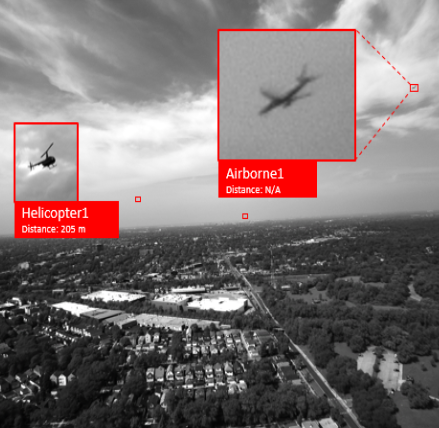
\includegraphics[width=0.5\textwidth]{figures/dataset-example-labeled.png}
        \caption{An example of airborne object dataset}
        \label{fig:airborne-object-example-1}
    \end{figure}
    \vspace{-2ex}
    %Seiring berkembangnya teknologi \emph{autonomous vehicles}, terdapat banyak keinginan untuk mengaplikasikan teknologi tersebut di berbagai bidang.
    %Salah satu aplikasi teknologi ini di bidang komersil adalah \emph{Amazon Prime Air}.
    %\emph{Amazon Prime Air} memanfaatkan \emph{Autonomous Aerial Vehicle} (AAV) untuk melakukan pengantaran barang dari warehouse ke rumah kostumer secara \emph{autonomous} \parencite{prime_air}.
    %Untuk melakukan hal ini, AAV yang digunakan harus mempunyai kemampuan penerbangan \emph{autonomous} yang mumpuni.

    %One of the most critical challenges in designing such a system is the 
    %ability to sense and avoid (SAA) obstacles. Although the airspace in 
    %which AAV operate is relatively sparse, there is still a risk of 
    %encountering static obstacles or airborne objects such as birds or drones.
    %In commercial application, such encounter would result not only in the AAV,
    %but also the item which the AAV carries.
    %Airborne objects pose a particularly difficult challenge as they often appear 
    %unexpectedly and approach rapidly from long distances due to their
    %inherent need for speed in flight.

    Autonomous Aerial Vehicle (AAV) have the potential to significantly impact 
    industries, particularly in commercial delivery. One notable example is Amazon 
    Prime Air, which is currently under development. Prime Air aims to deliver 
    goods from Amazon warehouses directly to customers \parencite{prime_air}. 
    To accomplish this, AAV require a reliable and efficient autonomy system.
 
    One of the most critical challenges in designing an AAV system is the 
    ability to sense and avoid (SAA) obstacles. While the airspace in which 
    AAVs operate may be relatively sparse, there is still risk of encountering 
    static obstacles or airborne objects such as birds or drones. In commercial 
    applications, such encounters can have consequences not only for the AAV 
    itself but also for the items it carries.  Ensuring effective SAA 
    capabilities is essential to mitigate these risks and safeguard both the AAV 
    and the valuable cargo it transports.


    Most SAA system of AAVs includes camera as their primary sensor.
    Cameras provide visual perception to the AAV, real-time, in the form of images. 
    These images must be processed by a computer vision algorithm to identify
    and localize the obstacles in it so that the AAV can estimate their 
    position and plan actions it needs to do to avoid them.
    There are other onboard sensing options such as LiDAR or radar, but cameras
    are more favored due to their lighter weight, cheaper price, 
    and relatively lower energy consumption compared to active sensors. 

    Airborne objects present a particularly challenging problem in SAA as they can 
    appear unexpectedly and approach rapidly from long distances due to their 
    inherent need for speed in flight. For this reason, it is important to detect airborne
    objects while they are still far away. Unfortunately, their far distance cause them 
    to appear very small on images. Figure \ref{fig:airborne-object-example-1} show an
    example of how airborne objects appear on images. In \textcite{aot_docs}, the airborne 
    objects can appear in the range of 4 to 1000 px on a $2048 \times 2448$ px image, that is,
    around 0.00008 - 0.01 \% of the image area.

    For reasons listed above, the computer vision algorithm to be implemented to detect these airborne objects, 
    must be able to detect small objects accurately. And not only that, it also must be able to do it in real-time.
    The fact that AAVs operating environments are outdoors, brings more trouble for the computer
    vision. Outdoor environment brings large complexity and additional variance to the image distribution, 
    making it almost impossible to handcraft feature extractor for it. This is where non-handcrafted
    feature extractors come in handy, particularly the deep learning approaches. Deep learning models
    have shown incredible abilities in handling complex data. Given enough training data, a deep learning
    model can craft itself feature kernels that can extract the objects in an image, despite being subjected
    to complex outdoor environment. For this reason, deep learning models gained prominence in addressing
    these challenges. 
    \begin{figure} [H]
        \centering
        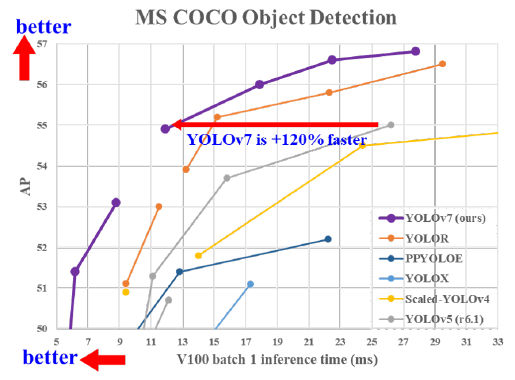
\includegraphics[width=0.75\textwidth]{figures/yolov7-coco.png}
        \caption{YOLOv7 performance on COCO dataset compared to other object detectors.}
        \label{fig:yolov7-coco}
    \end{figure}

    Introducing YOLOv7, a state-of-the-art convolutional neural network based real-time object detector \parencite{yolov7}.
    At the time of the proposal for this research was made (November 2022),
    YOLOv7 outperform both in speed and accuracy of all known real-time object detectors 
    with inference speed in the range of 5-160 FPS. It also has the highest accuracy (56.8\% AP) among
    object detectors with inference speed greater than 30 FPS on a V100 GPU. The capabilities of this cutting-edge architecture
    makes it well-suited for AAV computer vision system. However, all the performance metrics of YOLOv7
    mentioned before are obtained by training the model using COCO 2017 dataset. A dataset which 
    consist of general objects that people see in their daily life. COCO dataset is going to have
    very distinct distribution compared to airborne objects. As such, there would be a need for
    some modification to YOLOv7 so that it could detect airborne objects well.

    The topic of this research is about modifying YOLOv7 with objective of optimizing it to detect
    small objects, which extends to airborne objects. We experimented with some modification to 
    YOLOv7's bag-of-freebies, bag-of-specials, and network architecture. Then we benchmarked the
    modified models against the \textcite{aot_dataset}, and picked the model with the highest AP score
    that can perform inference in real-time.

    %For this to work, the computer vision algorithm must be able to be executed
    %in a real-time scenario, but also must be accurate enough 

    %Introducing YOLOv7. 

    %Dengan memilih kamera sebagai sensor, maka dibutuhkan suatu model computer vision untuk diaplikasikan pada kamera tersebut.
    %Objek - objek \emph{airborne} akan tampak sangat kecil pada kamera seperti yang dapat dilihat pada Gambar \ref{fig:airborne-object-example-1}.
    %Beberapa dataset kamera \emph{airborne} yang memiliki resolusi 20482448 pixel, objeknya dapat berukuran 4 (0.00008\% luas resolusi) hingga 1000 pixel (0.01\% luas resolusi) sehingga terlihat sangat kecil \parencite{aot_dataset}.
    %Oleh karena itu, dibutuhkan suatu model yang dapat mendeteksi objek - objek yang sangat kecil sehingga dapat mendeteksi objek \emph{airborne}.


    %YOLOv7 merupakan model state-of-the-art untuk melakukan pendeteksian objek secara real-time.
    %YOLOv7 memiliki akurasi tertinggi dari semua model pendeteksi objek dengan kecepatan deteksi 30 FPS (yang terpublikasi) pada GPU Nvidia V100.
    %Terdapat versi scaled dari YOLOv7 yang memiliki jumlah parameter yang lebih kecil dan dapat diaplikasikan pada device edge computing \parencite{yolov7}.
    %Oleh karena itu, YOLOv7 ini cocok untuk digunakan pada AAV di mana dibutuhkan suatu pendeteksi objek yang real-time.

\section{Problem Statement}
    
    %YOLOv7 bukan merupakan model deteksi objek umum sehingga YOLOv7 tidak didesain untuk melakukan deteksi objek kecil seperti objek-objek \emph{airborne}.
    %Oleh karena itu, dibuatlah rumusan masalah seperti berikut:
    %\begin{itemize}
    %    \item Apa solusi yang dapat diaplikasikan pada YOLOv7 agar kemampuan deteksi objek \emph{airborne}-nya dapat dioptimalisasi?
    %\end{itemize}
    YOLOv7 is not an object detection model specifically designed to detect small objects or airborne objects.
    Therefore, this research ask the following question.
    \begin{itemize}
        \item What modification can be done to YOLOv7 to improve its abilities in detecting airborne objects?
    \end{itemize}

\section{Purpose}
    The purpose of this research is to find modifications of YOLOv7 that would improve its ability in detecting airborne objects.
    %Adapun tujuan dari tugas akhir ini adalah untuk menemukan solusi untuk mengoptimisasi kemampuan YOLOv7 mendeteksi objek airborne.

\section{Problem Scope}
    % superintelligent AGI
    % solomonoff induction
    In this research, we want to formulate the scope of the problem such that the modifications applied
    on YOLOv7 would not lose its real-time detection ability and is still reasonably computable/trainable.
    Otherwise, we can just run a Solomonoff induction on airborne object data and call the result a modification
    of YOLOv7. Thus, we state the following scopes for the problem.
    \begin{itemize}%[noitemsep,topsep=0pt]
        \item YOLOv7 is used as the baseline for modifications. 
        \item The result of modification must be able to perform inference in real-time.
        \item The modified YOLOv7 must be trainable within a reasonable duration using the computational resource
        available, which is a computer which uses consumer GPU Nvidia RTX 2080 Ti.
    \end{itemize}
    %Optimisasi kemampuan deteksi objek kecil hanya akan dilakukan dengan memodifikasi YOLOv7.
    %Modifikasi yang diaplikasikan tidak boleh menyebabkan YOLOv7 untuk tidak dapat melakukan pendeteksian secara \emph{real time}.
    %Target pengaplikasian model ini adalah untuk AAV dengan \emph{computational resource} yang terbatas sehingga model hasil modifikasi harus cukup ringan untuk hal tersebut.
    %%Modifikasi yang mengubah arsitektur YOLOv7 secara signifikan sehingga tidak dapat melakukan pendeteksian secara \emph{real-time} tidak akan diaplikasian.
\cleardoublepage

% contents 2 tinjauan pustaka
\chapter{LITERATURE REVIEW}
\section{Theoretical Basis}
  \subsection{Object Detection Task}

  Object detection is a fundamental task in computer vision.
  It is a task that have 2 objective, localization and classification.
  Localization is about determining the spatial properties of an object, e.g. by
  enclosing them in bounding boxes. Classification is about determining the class of
  objects if they are animal, human, necromancer, or anything in the set of classes.

  To measure how well an object detection algorithm or model perform, computer vision
  researchers defined metrics to measure how fit a model prediction to an object
  and to measure how well the model perform across all objects. Example of those metrics are IoU and mAP.

  \subsubsection{Intersection Over Union (IoU)}
   \begin{figure}[H]
        \centering
        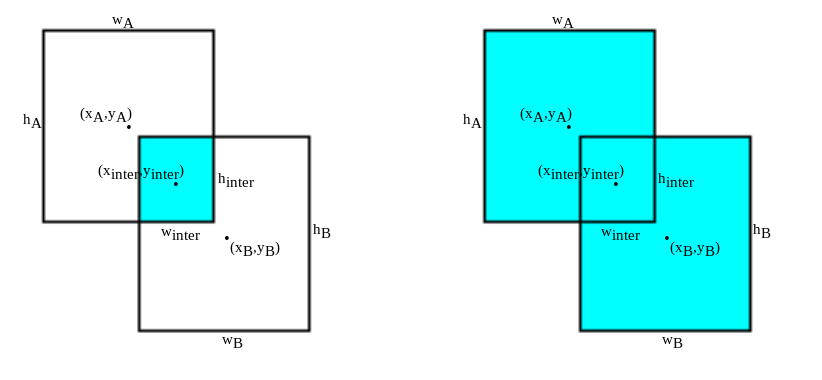
\includegraphics[width=0.7\textwidth]{figures/inter-union.png}
        \caption{Intersection and Union of 2 Bounding Boxes}
        \label{fig:inter-union}
    \end{figure}
  Intersection over union (IoU) is a widely used metrics to determine how fit a predicted bounding box against the true bounding box.
  It is done by calculating the area of the intersection between the predicted and dividing it by the area of the
  union of those 2 boxes. 
  
  The IoU of 2 bounding boxes A and B can be calculated using the following way:
  \begin{itemize}
    \item Calculate the area of intersection of A and B. 

    Let $(x_A,y_A)$ and $(x_B,y_B)$ be coordinates of the center of the box A and B respectively,
    and let $(w_A,h_A)$ and $(w_B,h_B)$ be widths and heights of the center of the bow A and B.

    The calculation for the area of intersection can be done like this:
    \begin{align*}
      x_{\text{{inter}}} &= \max(x_A, x_B) \\
      y_{\text{{inter}}} &= \max(y_A, y_B) \\
      w_{\text{{inter}}} &= \min(x_A + w_A, x_B + w_B) - x_{\text{{inter}}} \\
      h_{\text{{inter}}} &= \min(y_A + h_A, y_B + h_B) - y_{\text{{inter}}} \\
      \text{Area}_{\text{inter}} &= w_{\text{{inter}}} \times h_{\text{{inter}}}
    \end{align*}
    \item Calculate the area of union.

    From set theory, we know that $|A \cup B| =|A| + |B| - |A \cap B| $.
    This also applies when calculating the area of union.
    \begin{align*}
      \text{Area}_{union} &= \text{Area}_A + \text{Area}_B - \text{Area}_{\text{inter}}\\
      \text{Area}_{union} &= w_A\times h_A + w_B\times h_B  - \text{Area}_{\text{inter}}
    \end{align*}
    \item Finaly, calculate IoU
    \begin{equation}
      IoU = \frac{\text{Area}_{\text{inter}}}{\text{Area}_{\text{union}}}
    \end{equation}
  \end{itemize} 

  \subsubsection{Mean Average Percision (mAP)}
  Average Precision (AP) is a popular metrics used to measure the capability of an object detection model
  for a given dataset. The main advantage of using AP are its ability to capture the precision recall
  tradeoff and its independence towards confidence threshold. AP has these 2 advantage as an effect of the way 
  it is calculated.

  To calculate AP, precision and recall area under the curve (AUC) must be calculated first.
  Precision is defined as
  \begin{equation}
    P(\mathbb{S}_c,h,\tau,\epsilon) = \dfrac{\left|\left\{(\hat{B},x) \in \mathbb{S} :\ \exists B \in h(x,\tau)_c,\ IoU(\hat{B},B) > \epsilon  \right\}\right|}{\left| \{B \in h(x,\tau)_c\} \right|}
    \label{eq:precision}
  \end{equation}
  \begin{align*}
    \text{Where}~ h &=  \text{hypothesis/model that predict bounding boxes}\\%\tau}\\
    \mathbb{S}_c &= \text{set of bounding boxes of class $c$ in dataset paired with their respective image}\\
    h(x,\tau)_c &= \text{bounding boxes predicted by $h$ with class $c$}\\
    \tau &= \text{confidence threshold for $h$} \\
    \epsilon &= \text{$IoU$ threshold for a positive prediction}\\
    B &= \text{Bounding box}\\
    x &= \text{image}
  \end{align*}
  and for recall, it is defined as
  \begin{equation}
    R(\mathbb{S}_c,h,\tau,\epsilon) = \dfrac{\left|\left\{(\hat{B},x) \in \mathbb{S} :\ \exists B \in h(x,\tau)_c,\ IoU(\hat{B},B) > \epsilon  \right\}\right|}{\left| \mathbb{S}_c \right|}
    \label{eq:recall}
  \end{equation}
  Then we define the precision recall curve as a parametric function
  \begin{equation}
    PR(\tau) = \left( R(\mathbb{S}_c,h,\tau,\epsilon),P(\mathbb{S},h,\tau,\epsilon) \right)
    \label{eq:pr}
  \end{equation}
  Using equation \ref{eq:pr}, $PR$ curve in Figure \ref{fig:pr-curve} can be generated using $0 \leq \tau \leq 1$
  \begin{figure}[H]
        \centering
        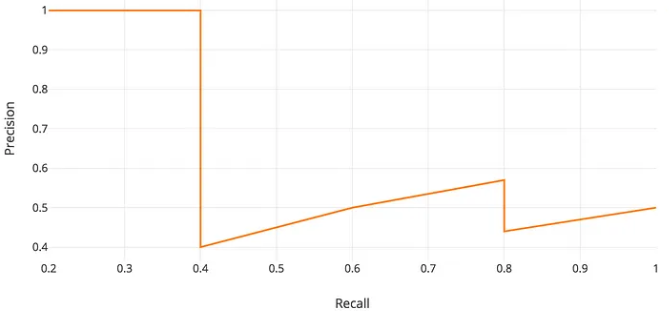
\includegraphics[width=0.75\textwidth]{figures/pr-curve.png}
        \vspace{-1ex}
        \caption*{Source: \textcite{map-hui}}
        \vspace{-1ex}
        \caption{PR Curve Generated by Varying $\tau$}
        \label{fig:pr-curve}
  \end{figure}
  Before calculating the AP however, the curve in Figure \ref{fig:pr-curve} is usually interpolated using Equation \ref{eq:pr-inter},
  which relies on Equation \ref{eq:pr-functionization} that transformed $PR$ curve to a functional relation of R to P.
  The interpolated curve can be seen on \ref{fig:pr-interp}

  \begin{align}
    \label{eq:pr-inter}
    p_{inter}(r) &= \max_{\bar{r}>r} p(\bar{r})\\
    \label{eq:pr-functionization}
    \text{Where}~p(\bar{r}) &= \max \left\{p : \forall (r,p) \in \{PR(\tau) , 0\leq\tau\leq 1\}, r=\bar{r}\right\}%\text{precision given recall value in Figure \ref{fig:pr-curve}}
  \end{align}

  \begin{figure}[H]
        \centering
        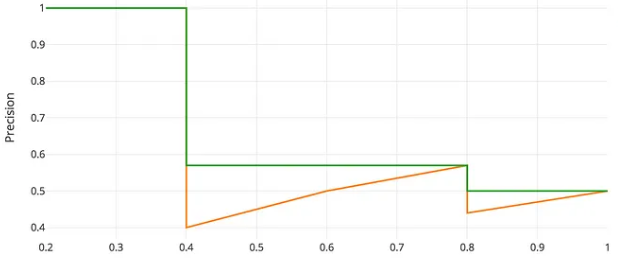
\includegraphics[width=0.75\textwidth]{figures/pr-interp.png}
        \vspace{-1ex}
        \caption*{Source: \textcite{map-hui}}
        \vspace{-1ex}
        \caption{PR Curve Interpolated}
        \label{fig:pr-interp}
  \end{figure}
  The AP, which is the area under the curve then can be calculated using the following integral:
  \begin{equation}
    AP = \int_{0}^{1} p_{inter}(r) \, dr
  \end{equation}

  When calculating AP, the $IoU$ threshold for positive detection is usually predefined. As example,
  for AP@50, we set the $\epsilon$ in Equation \ref{eq:precision} and \ref{eq:recall} to 50\%. And for 
  AP@75, the $\epsilon$ is set to 75\%.

  The AP calculation so far only works for a single class. To have a multiclass metric, we use mAP
  which is calculated as the average AP across all classes in the dataset.
  \begin{equation}
    mAP@X = \frac{1}{|\text{classes}|} \sum_{c\in \text{classes}} AP_c@X
  \end{equation}
  %\begin{align*}
  %  \text{Where}~p(r) &= \text{precision given recall value in Figure \ref{fig:pr-curve}}
  %\end{align*}
  %Traditionally, object detection algorithms relied on handcrafted feature kernels and machine learning techniques. 
  %However, deep learning has become a popular solution for object detection by the use of Convolutional Neural Networks (CNN)
  %to learn feature kernels automatically. With the usage of deep learning, object detection task
  %had significant advancement in terms of accuracy and efficiency.


  \subsection{YOLO Family Architecture}
  YOLO is an abbreviation of "You Only Look Once" which describes what kind of neural network YOLO
  is, a single stage object detector. It means that this architecture predicts regions 
  and classes both at once. In contrast, two-stage detector predicts objects' regions first
  and then predicts their classes. Detecting objects in a single-stage manner is what gave YOLO
  architecture the ability to infer in real-time. This is possible due to how YOLO architecture
  was designed. YOLO architecture consist of 3 main part, the head, the neck, and the backbone.

    %Arsitektur famili YOLO pada dasarnya terbagi akan 3 bagian yaitu \emph{head}, \emph{neck}, dan \emph{backbone}.
    %Setiap bagian ini mempunyai fungsi masing-masing.
   
    %Berikut adalah penjelasan fungsi dan cara kerja dari ketiga bagian tersebut.
    \subsubsection{Backbone}
    The backbone is the network that extract features from the inputted image.
    Typically, the backbone is composed of deep neural network layers that progressively 
    downsample the spatial dimensions of the input while increasing the number of 
    learned features or meaningful abstraction of the data.

    The implementation of backbone in YOLO usually varies from one version to another.
    As example, \textcite{yolov2}'s YOLOv2 implemented Darknet-19 network as backbone, 
    \textcite{yolov3}'s YOLOv3 implemented Darknet-53, \textcite{yolov4}'s YOLOv4
    with their CSP-Darknet-53, or \textcite{vityolo} with their non-CNN (Transformer) backbone.
    Each of these network has their own has their own advantages and disadvantage when
    it comes to accuracy, memory requirement, or latency.


    %\emph{Backbone} dari YOLO merupakan bagian yang mengekstrak fitur dari citra yang diinputkan.
    %Hasil ekstraksi fitur ini akan diinputkan pada \emph{neck} yang kemudian akan di\emph{upsampling} olehnya.
    %Model-model YOLO dapat menggunakan \emph{feature extractor} dari model-model klasifikasi citra sebagai \emph{backbone}-nya.
    %Sebagai contoh, salah satu varian YOLO, YOLO-Z menggunakan DenseNet sebagai \emph{backbone}-nya sedangkan arsitektur YOLO dasarnya, YOLOv5 menggunakan \emph{backbone} YOLOv5v7.0 \parencite{yoloz}.
    \subsubsection{The Neck}
  
    \begin{figure}[H]
        \centering
        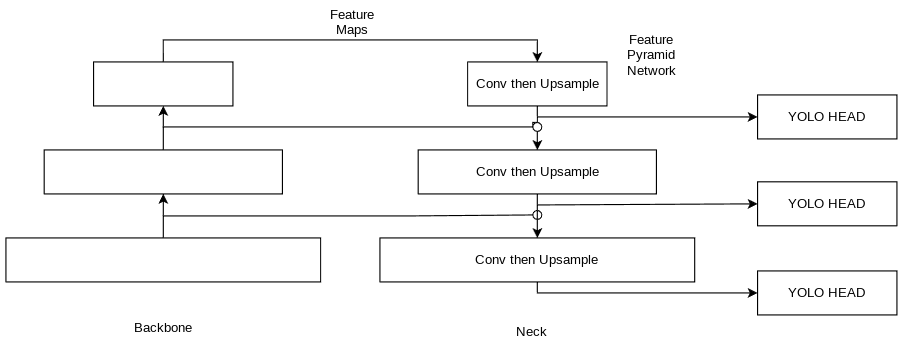
\includegraphics[scale=0.6]{figures/yolo-architecture-rough.png}
        \caption{Feature Pyramid Network in YOLOv3}
        \label{fig:yolofpn}
    \end{figure}

    The neck is the intermediate network between backbone and head.
    The main function of the neck is to enhance features extracted by the backbone.
    Specific implementation of neck for each YOLO architecture is different one to the other.
    Some neck implementation try to combine feature maps across different prediction scales of YOLO network.

    \textcite{yolov3} was the first to introduce YOLO prediction in multiple scale in YOLOv3.
    To enhance the feature maps with using information across scales, YOLOv3 fuses features 
    from multiple parts of the backbone before up sampling them as seen on Figure \ref{fig:yolofpn}. 
    This type of neck network is called Feature Pyramid Network (FPN). 
    A further improvement was made by \textcite{yolov4} with their YOLOv4 by introducing Path 
    Aggregation Network (PANet) for the neck. 
    With PANet, feature are fused back to higher scale by adding another FPN-like layer after the original FPN
    but with reverse direction.
    %The way it works is by taking feature maps, not only in the last output layer of the
    %backbone, but also in multiple parts of the backbone.
    %For example, YOLOv4 uses PANet to enhance and combine features across different scales
    %of prediction.
  
    %\emph{Neck} dari YOLO merupakan \emph{layer-layer} dimana \emph{head} YOLO mengambil fitur untuk dilakukan deteksi \emph{bounding box}.
    %Pada YOLOv3 \textcite{yolov3}, arsitektur \emph{neck} dibuat menyerupai \emph{Feature Pyramid Network} (FPN) seperti pada Gambar \ref{fig:yolofpn}. 
    %Pada versi-versi YOLO selanjutnya, bentuk \emph{neck} ini tidak banyak berubah dan pada dasarnya tetap mempertahankan bentuk \emph{pyramid}-nya.
  
    %Penaikkan tingkatan \emph{pyramid} dari FPN merupakan \emph{upsampling} dari \emph{feature map} yang dihasilkan \emph{backbone}.
    %Output tiap tingkatan pada FPN di \emph{neck} inilah yang diinputkan pada \emph{head} YOLO. 
    %Melakukan prediksi pada tingkatan \emph{upsampling} yang berbeda-beda dapat membuat \emph{neural network} mendapatkan lebih banyak informasi semantik dan informasi yang lebih detail sehingga dapat lebih akurat dalam mendeteksi objek besar maupun kecil.
 

  
    \subsubsection{The Head and The Anchors}
    \begin{figure}[H]
        \centering
        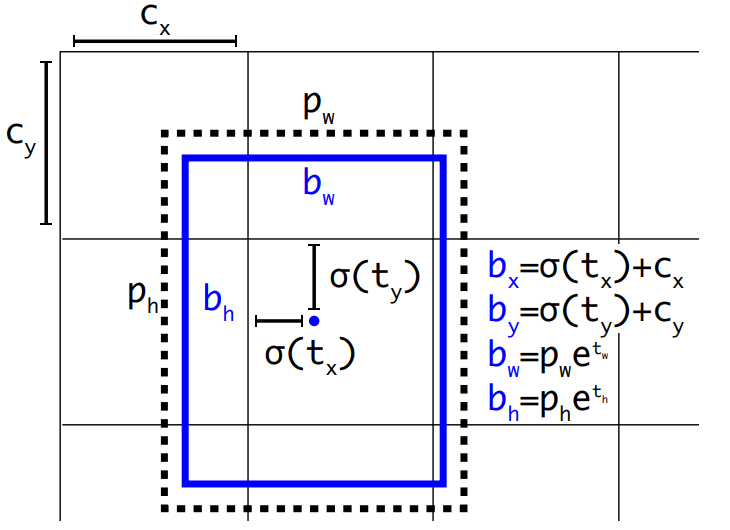
\includegraphics[width=0.5\textwidth]{figures/anchorbox.png}
        \caption*{Source: \textcite{yolov3}}
        \caption{Head layer predict anchor box and its offsets from lattice of the feature grid }
        \label{fig:anchorbox}
    \end{figure}
    The head is where the object detection happens. Extracted and enhanced features of the image is fed to the head 
    in multiple different scales. For each scale, the head will predict a box for each $N \times N$
    lattice point on feature map's grid. In total, each layer will output a tensor with size
    $N_k \times N_k \times [A_k \times (4+1+C)]$ where $N_k$ is the size of feature map grid at the $k$-th scale,
    $A_k$ is the number of anchors for that scale, 4 is for the four offsets $[t_x, t_y, t_w, t_h]$ in figure 
    \ref{fig:anchorbox}, 1 is for the objectness score for the grid, and $C$ is for the number of classes it has
    to predict.
    
    Most of YOLO family architecture head utilizes anchor boxes to assist bounding box prediction.
    This technique is used in \textcites{yolov2}{yolov3}{yolov4}{scaledyolov4}{yolov5}{yolor}{yolov7}.
    Instead of directly predicting the size and position of the bounding box, YOLO head predicts 
    the offsets for each anchor boxes assigned to the head, then it utilizes the objectness score to pick
    which result  of these anchor boxes to be used.
    Using anchor boxes allows the neural network to converge more quickly because it provides
    a prior knowledge of the dataset before training.
    
    %The way it works is that, there will be a preset of detection boxes.
    %Arsitektur famili YOLO yang dipublikasikan setelah YOLOv2 terus menggunakan \emph{anchor box} untuk melakukan deteksi \parencites{yolov2}{yolov3}{yolov4}{scaledyolov4}{yolov5}{yolor}{yolov7}.
    %\emph{Anchor boxes} merupakan beberapa \emph{Bounding Box} yang telah terdefinisikan. 
    %Arsitektur YOLO akan memprediksi probabilitas \emph{anchor box} berada pada suatu koordinat latis beserta dengan \emph{offset anchor box} tersebut untuk menepatkan \emph{anchor box} pada objek yang dideteksi.
    %Penggunaan \emph{anchor box} ini dapat meningkatkan akurasi deteksi karena \emph{neural network} hanya perlu mencari titik tengah objek dan \emph{error} dimensi \emph{boudning box} dengan menggunakan \emph{offset} \parencite{yolov3}.
    %Hal ini lebih sederhana daripada mencari titik-titik \emph{bounding box} secara independen sehingga lebih mudah untuk dipelajari oleh \emph{neural network}.
  
    %Prediksi \emph{bounding boxes} terjadi di bagian \emph{head} dari arsitektur YOLO.
    %Bagian \emph{head} dari YOLO akan mengambil beberapa hasil \emph{upsampling} yang terjadi pada \emph{neck} YOLO, dan kemudian melakukan prediksi \emph{anchor boxes} dari hasil tersebut.
    %Hasil prediksi \emph{Head} YOLO pada suatu tingkatan \emph{upsampling} berupa tensor dengan ukuran $N\times N \times [A\times(4+1+C)]$ dengan $N$ sebagai dimensi hasil \emph{upsampling}-nya, $A$ sebagai jumlah \emph{anchor boxes} untuk \emph{scaling} tersebut, dan $C$ sebagai jumlah kelas prediksi.
    %Angka 4 merepresentasikan 4 \emph{offset} $b_x, b_y, b_w, b_h$ seperti pada Gambar \ref{fig:anchorbox} dan angka 1 merepresentasikan \emph{objectness score} dari prediksi \emph{bounding box}.

    \subsubsection{Loss Function}
    The goal of a YOLO architecture is to (1) predict if an object exist or not, (2) predict the bounding box of such object,
    and (3) predict the class of the object. These 3 loss functions that correspond to those objectives are called 
    objectness loss, box loss, and class loss respectively. To update the weights on training, the total loss is calculated as 
    the weighted sum of those 3 losses.
    %\begin{equation}
    %  L_{box} = \sum_{k=0}^{n}\sum_{i,j=0}^{N_k}\sum_{m=0}^{A_k} \mathbbm{1}_{k,i,j,m}^{obj} -IoU(gt(x), M(x)_{k,i,j,m})
    %\end{equation}
    In original YOLO, the loss functions were defined like the following.

    For localization loss, it is described by equation \ref{eq:yolo-box-loss}.
    \begin{equation}
      L_{box} = \sum_{i=0}^{S^2} \sum_{j=0}^B \mathbbm{1}_{ij}^{obj} \left[(x_i - \hat{x}_i)^2 + (y_i - \hat{y}_i)^2 + (\sqrt{w_i}-\sqrt{\hat{w}_i})^2 + (\sqrt{h_i}-\sqrt{\hat{h}_i})^2\right] \\
      \label{eq:yolo-box-loss}
    \end{equation}
    \begin{align*}
    \text{Where}~S^2  &= \text{the total number of grid cells in the output,}\\
    B &= \text{ the total number of anchor box per grid cells,}\\
    \mathbbm{1}_{ij}^{obj} &= \begin{cases}
                                1, & \text{if object present in grid}\\
                                0, & \text{otherwise,}
                              \end{cases} 
                              \\
    (x_i, y_i) &= \text{the predicted coordinates of the center of object i}\\
    (\hat{x}_i, \hat{y}_i) &= \text{the ground truth coordinates of the center of object}\\
    (w_i, h_i) &= \text{the predicted width and height of object i}\\
    (\hat{w}_i, \hat{h}_i) &= \text{the ground truth width and height of object}
      %\text{the indicator variable that has value 1 if object is present in the grid and 0 otherwise.}
    \end{align*}
    %$\mathbbm{1}_{ij}^{obj}$ is the indicator variable that has value 1 if object is present in the grid and 0 otherwise.
    %$(x_i, y_i)$ and $(\hat{x}_i, \hat{y}_i)$ are the predicted and ground truth coordinates of the center of object $i$.
    %$(w_i, h_i)$ and $(\hat{w}_i, \hat{h}_i)$ are the predicted and ground truth widths and heights of object $i$.
    For objectness loss, described by equation \ref{eq:yolo-obj-loss}
    \begin{equation}
      L_{obj} = \sum_{i=0}^{S^2} \sum_{j=0}^B \mathbbm{1}_{ij}^{obj}(C_i - \hat{C}_i)^2  + \alpha \mathbbm{1}_{ij}^{noobj}(C_i - \hat{C}_i)^2
      \label{eq:yolo-obj-loss}
    \end{equation}
    \begin{align*}
    Where~\mathbbm{1}_i^{\text{noobj}} &=\begin{cases} 
                                          1, & \text{if object assigned to anchor j}\\
                                          0, & \text{otherwise} 
                                         \end{cases}\\
          (C_i,\hat{C}_i) &= \text{predicted and ground truth confidence score for objectness of anchor}
    \end{align*}
    %$(C_i, \hat{C}_i)$ are the predicted and ground truth confidence scores for objectness of anchor $i$,
    And for class loss, described by \ref{eq:yolo-class-loss}
    \begin{equation}
      L_{class} = \sum_{i=0}^{S^2} \mathbbm{1}_{ij} \sum_{c \in classes} (p_i(c) - \hat{p}_i(c))^2
      \label{eq:yolo-class-loss}
    \end{equation}
    Where $(p_i(c), \hat{p}_i(c))$ are the predicted and ground truth class probabilities for class $c$ for object $i$.

    The three losses combined to the final loss function in equation \ref{eq:yolo-loss}
    \begin{equation}
      L = \lambda_{box}L_{box} + \lambda_{obj}L_{obj} + \lambda_{class}L_{class}
      \label{eq:yolo-loss}
    \end{equation}
    \begin{align*}
      Where~\lambda_{box} &= \text{the weight for localization,}\\
      \lambda_{obj} &= \text{weight for objectness}\\
      \lambda_{class} &= \text{weight for class}
    \end{align*}
    These 3 $\lambda$-s can be tuned to optimize the performance of a YOLO network.

    %\begin{equation}
    %  L_{box} = \sum_{i=0}^{S^2}\sum_{j=0}^B   \mathbbm{1}_{ij}^{obj} (x_i-\hat{x}_i)^2 + (y_i-\hat{y}_i)^2 + (\sqrt{w_i}-\sqrt{\hat{w}_i})^2 + (\sqrt{h_i}-\sqrt{\hat{h}_i})^2 
    %\end{equation}
      %L_{box} = \sum_{k=0}^{n}\sum_{i,j=0}^{N_k}\sum_{m=0}^{A_k} \mathbbm{1}_{k,i,j,m}^{obj} -IoU(gt(x), M(x)_{k,i,j,m})

    %\begin{equation}
    %  L_{box} = 1
    %\end{equation}

  
      
  \subsection{YOLOv7}
  As said in section \ref{section:background}, YOLOv7 is the state-of-the-art real-time object detector.
  It was made by the authors of YOLOv4, and by the time it was published (july 2022), it surpassed all 
  known real-time object detectors both in speed and accuracy. To achieve this, YOLOv7 implemented some new
  changes and addition to the neural network. 
  \subsubsection{Backbone}

%  \vspace{-2ex}
  %\begin{figure}[H]
  %    \centering
  %    \subfigure[ELAN block]{
  %    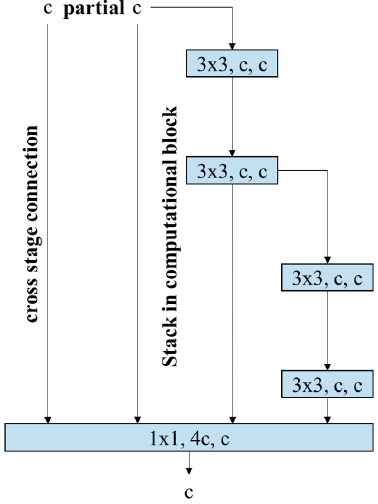
\includegraphics[width=0.2\textwidth]{figures/elan-block.png}
  %    \label{fig:elan-block}
  %    }
  %    \subfigure[FIGTOPCAP][First two ELAN blocks in YOLOv7]{
  %    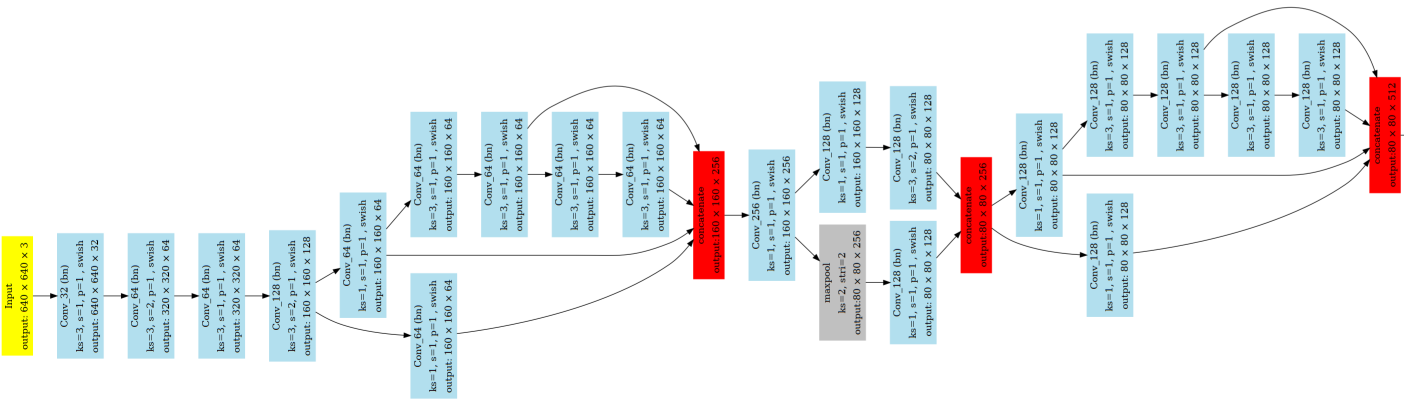
\includegraphics[width=0.75\textwidth]{figures/yolo-elan-blocks.png}
  %    \label{fig:elan-yolo}
  %    }
  %    \caption{ELAN in YOLOv7}
  %    \label{fig:elan}
  %\end{figure}
  \begin{figure}[H]
    \centering
    \begin{subfigure}[c][][c]{.35\textwidth}
        %%%\vspace{0pt}
        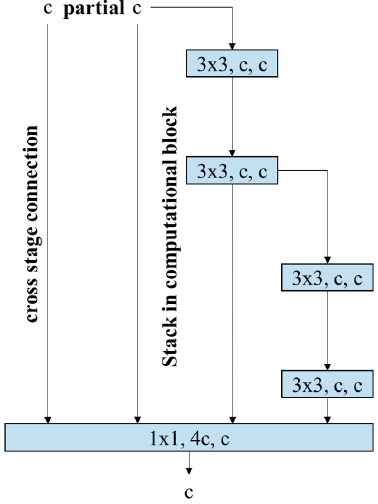
\includegraphics[width=1\linewidth]{figures/elan-block.png}
        \caption{ELAN block}
        \label{fig:elan-block}
    \end{subfigure}

    \begin{subfigure}[c][][c]{.9\textwidth}
        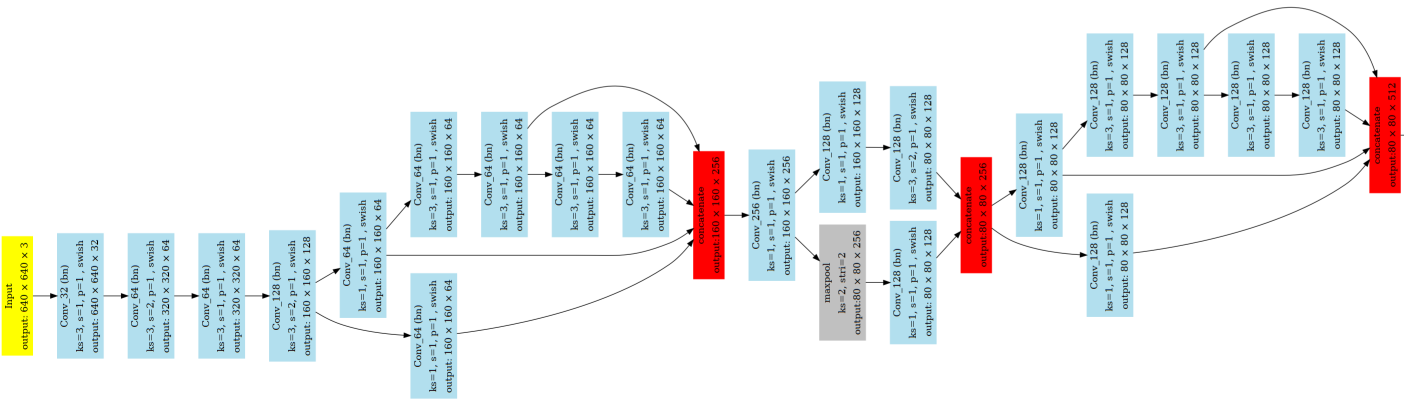
\includegraphics[width=1\linewidth]{figures/yolo-elan-blocks.png}
        \caption{First two ELAN blocks in YOLOv7}
        \label{fig:elan-yolo}
    \end{subfigure}
    \caption*{Source: \textcite{yolov7}}
    \caption{ELAN in YOLOv7}
    \label{fig:elan}
  \end{figure}

  %remove this negative vspace if buku TA kurang panjang

  YOLOv7 implemented the Efficient Layer Aggregation Network (ELAN) and Extended-ELAN (E-ELAN) as the backbone of its network. 
  ELAN is a convolutional neural network that was designed to extract features efficiently 
  by controlling the shortest longest gradient path in the network \parencite{elan}.
  This choice of backbone allows YOLOv7 to perform prediction more accurately despite having fewer number of parameters. 
  Figure \ref{fig:elan-yolo} shows how ELAN block in Figure \ref{fig:elan-block} implemented in YOLOv7.

  \subsubsection{Label Assignment Strategy and Auxilary Head}
  \begin{figure}[H]
      \centering

      \begin{subfigure}[][][t]{0.5\textwidth}
        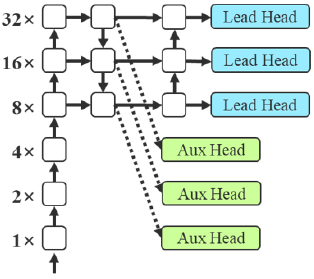
\includegraphics[width=1\linewidth]{figures/auxilary-head.png}
        \caption{Auxliary heads attachment in YOLOv7}
        \label{fig:aux-head}
      \end{subfigure}

      \begin{subfigure}[][][t]{0.4\textwidth}
        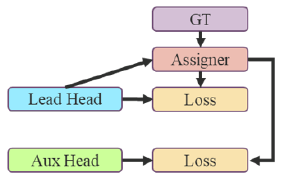
\includegraphics[width=1\linewidth]{figures/lead-head-assigner.png}
        \caption{Lead guided label assignment}
        \label{fig:lead-head}
      \end{subfigure}\hfill
      \begin{subfigure}[][][t]{0.4\textwidth}
        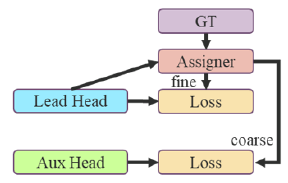
\includegraphics[width=1\linewidth]{figures/coarse-to-fine.png}
        \caption{Coarse-to-fine lead guided label assignment}
        \label{fig:coarse-to-fine}
      \end{subfigure}
      \caption*{Source: \textcite{yolov7}}
      \caption{YOLOv7 Label Assignment Strategy with Auxilary Heads}
      \label{fig:labelassigner}
  \end{figure}
  SimOTA, first introduced in YOLOX, is an algorithm to approximate Optimal Transport Assignment (OTA)
  in a faster way. \textcite{yolox} introduced SimOTA in YOLOX because OTA was deemed too slow to compute
  as it was increasing the training time by 25\%. YOLOv7 also implemented SimOTA for its dynamic label assigner.

  YOLOv7 deep supervised its training process by attaching auxilary heads to its neural network
  as seen on Figure \ref{fig:aux-head}.
  These auxilary heads is only used on training, on inference, they are removed from the neural network
  to improve latency, only the lead head is kept. There is a problem however with assigning labels
  to the auxilary and lead heads. Most object detection networks that utilizes auxilary heads have 2
  independent label assigners, one for auxilary heads and one for lead heads. YOLOv7 done things differently.


  YOLOv7 proposed 2 way of assigning labels to auxilary and lead heads. Lead head guided label assignment (Figure \ref{fig:lead-head}) and
  coarse-to-fine lead head guided assignment (Figure \ref{fig:coarse-to-fine}). For lead head guided label assignment, the assigner gives a copy
  of lead heads' label assignment to the auxilary heads. For coarse-to-fine lead head guided assignment, the 
  assigner works like lead head guided assigner but gives coarse label assignment to auxilary head. Coarse label
  assignment is done by relaxing the positive sample constraints of the assigner. \textcite{yolov7} find that coarse-to-fine
  label assignment produces the greatest AP scores.
  
  Due to the relaxed constraints, coarse label assignment to auxilary heads assigns more positive labels the auxilary heads' grids. 
  This way, the network will learn more to recall.
  On inference, this recall ability would be filtered by the lead head to produce accurate prediction.

  \subsubsection{Reparameterization}
  YOLOv7 utilized RepConv and YOLOR implicit layers in its network.
  In addition to that, YOLOv7 also uses Convolution-BatchNorm layer.
  These layers can be reparameterized after training to simplify the neural network, thereby reducing
  latency and memory usage but not hurting inference performance.

  The reparameterization of YOLOR implicit layers can be done after training by computing
  some mathematical simplification of the implicit layers.
  For combination of YOLOR\textsuperscript{+}--Convolution--YOLOR\textsuperscript{+} layers, it can be reparameterized like the following.
  \begin{align*}
    x_{n+1} &= W(x_{n}+g_1(z_1)) + b + g_2(z_2)\\
    &= W(x_{n}) + (W(g_1(z_1)) + b + g_2(z_2))\\
    &= W(x_{n}) + b'
  \end{align*}
  Observe that the reparameterization combined 3 layers into a single convolution layer with bias. Then, For combination of
  YOLOR*--Convolution--YOLOR* layers:
  \begin{align*}
    x_{n+1} &= (W(g_1(z_1)x_n)+b)g_2(z_2)\\
    &= g_2(z_2)g_1(z_1)W(x_n) + b g_2(z_2)\\
    &= W'(x_n) + b'
  \end{align*}
  And finally for Convolution-BatchNorm:
  \begin{align*}
    x_{n+1} &= ((W(x_n)+b)-m)/s\\
    &= (W(x_n) + (b-m))/s\\
    &= (W/s)(x_n) + (b-m)/s\\
    &= W'(x_n) + b'
  \end{align*}

  In summary, YOLOR\textsuperscript{+}--Conv--YOLOR\textsuperscript{+} will be replaced with the original convolutional layer $W$ but with bias $W(g_1(z_1)) + b + g_2(z_2)$.
  YOLOR*--Conv--YOLOR* layers will be replaced with a convolutional $g_2(z_2)g_1(z_1)W$ and bias $b g_2(z_2)$.
  And Conv--BatchNorm will be replaced with a convolutional $W/s$ and bias $(b-m)/s$.
  %TODO: reparam equation here
    %YOLOv7 merupakan pendeteksi objek \emph{real time} dengan skor akurasi tertinggi pada dataset COCO di tahun 2022.
    %Pada YOLOv7, dilakukan beberapa perubahan untuk meningkatkan akurasi dan kecepatan deteksinya.
    %Perubahan-perubahan tersebut dilakukan pada arsitekturnya dan pada \emph{bag-of-freebies}-nya.
  
    %Perubahan arsitektur dilakukan pada \emph{backbone}. YOLOv7 menggunakan \emph{Extended Efficient Layer Aggregation Network} (E-ELAN) sebagai \emph{backbone}, berbeda dengan leluhurnya YOLOv4 yang menggunakan CSP-Darknet.
    %E-ELAN merupakan arsitektur \emph{neural network} yang efisien karena E-ELAN didesain dengan mengontrol \emph{gradient path} terpanjang yang terpendek.
    %Karena efisiensinya, arsitektur E-ELAN ini dapat meningkatkan kecepatan deteksi dan akurasi. \parencite{yolov7}
  
    %\emph{Bag-of-freebies} merupakan kumpulan metode peningkatan akurasi yang tidak meningkatkan \emph{cost inferrence} \parencite{yolov4}. 
    %Pada YOLOv7, ditambahkan beberapa \emph{bag-of-freebies} yang dapat dilatih seperti \emph{re-parameterized convolution} dan \emph{extra auxilary head} di tengah-tengah \emph{neural network}.
    %Selain kedua itu, YOLOv7 juga menambahkan \emph{trainable bag-of-freebies} dari YOLOR seperti EMA, \emph{Implicit Knowledge}, dan \emph{conv-bn topology Batch Normalization} \parencite{yolov7}.
    %Introducing YOLOv7, a state-of-the-art deep learning based real-time object detector \parencite{yolov7}.
    %At the time of the proposal for this research was made (November 2022),
    %YOLOv7 outperform both in speed and accuracy of all known real-time object detectors 
    %with inference speed in the range of 5-160 FPS. It also has the highest accuracy (56.8\% AP) among
    %object detectors with inference speed greater than 30 FPS on a V100 GPU. The capabilities of this cutting-edge architecture
    %makes it well-suited for AAV computer vision system. However, all the performance metrics of YOLOv7
    %mentioned before are obtained by training the model using COCO 2017 dataset. A dataset which 
    %consist of general objects that people see in their daily life. COCO dataset is going to have
    %very distinct distribution compared to airborne objects. As such, there would be a need for
    %some modification to YOLOv7 so that it could detect airborne objects well.


  \subsection{Anchor Recalculation}
  \label{section:anchor_recalc_study}
  Anchor recalculation is a common method of introducing prior distribution of the dataset to an anchor-based object
  detection networks. Most of the time, anchors provided by pretrained YOLO weights are optimized for the common metrics
  dataset such as COCO2017 or VOC2012. Thus, recalculating anchor can help the neural network learn faster.

  There are multiple ways of recalculating anchors. Some of them can be performed before training or during training.
  Most of pre-training anchor recalculation method involves with clustering the anchors to the dataset. This is done by
  using clustering algorithm such as K-means, Gaussian Mixture, and many others. Recalculating anchor on training is 
  a little more complex to do as it will involve some loss function or architectural change on the object detection neural network.
  \textcite{anchoropt} for example add additional layer on detection part of object detectors that is connected to anchor modifiers such that
  the anchors will also be updated during training. \textcite{yolor} mentioned that the implicit multiplication layer of their network
  can be purposed for anchor refinement.

  %\emph{Anchor box} dari model-model \emph{pre-trained} YOLO pada umumnya mengoptimisasi \emph{anchor box} modelnya pada dataset COCO.
  %Ukuran \emph{anchor box} yang akan digunakan pada model YOLO dapat dikonfigurasikan agar lebih sesuai dengan dataset yang akan digunakan untuk melatih model YOLO.
  %Penyesuaian ini dapat meningkatkan IoU(\emph{Intersection Over Union}) prediksi model dengan \emph{ground truth} sehingga meningkatkan akurasi.

  %Penyesuaian anchor box dapat dilakukan pada saat sebelum training atau pada saat training.
  %Penyesuaian anchor box sebelum training dapat dilakukan dengan cara mengkonfigurasi secara manual tiap ukuran \emph{anchor box} atau dengan menggunakan algoritma \emph{clustering}.
  %Penggunaan algoritma \emph{clustering} akan lebih baik karena setiap ukuran \emph{anchor box}-nya disesuaikan dengan pengelompokan-pengelompokan ukuran \emph{bounding box} natural yang terdapat pada dataset.
  %Untuk penyesuaian saat training, dapat digunakan algoritma dari \textcite{anchoropt}.
  %Algoritma ini akan mengoptimisasi ukuran-ukuran anchor bukan hanya berdasarkan dataset, namun berdasarkan kemampuan dari neural network pendeteksi objeknya.
  %Untuk melakukan hal tersebut, algoritma ini akan memanfaatkan back propagation localization loss untuk rekalkulasi anchor.

  \subsection{Mosaic Augmentation}
  \label{section:mosaic_study}
  \begin{figure}[H]
    \centering
    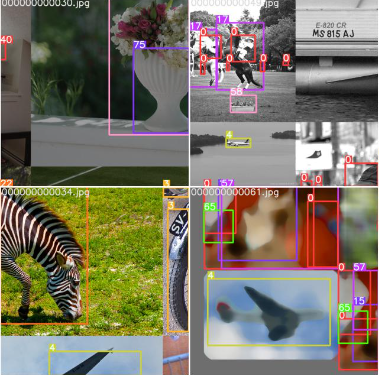
\includegraphics[width=0.5\textwidth]{figures/mosaic-aug.png}
    \caption*{Source: \textcite{yolov5}}
    \caption{Four example of mosaic augmentation \parencite{yolov5}}
    \label{fig:mosaic}
  \end{figure}
  Mosaic augmentation was introduced in Ultralytics' implementation of YOLOv3 \parencite{mosaic_aug}.
  This augmentation technique will randomly pick 4 images of the dataset, and tile them randomly into one image like in \ref{fig:mosaic}.
  It's called mosaic due to how the result of the augmented image have mosaic-like appereance.
  \textcites{cspnet}{yolov4}{yolov5} reported increase in accuracy after applying mosaic augmentation.
  %Augmentasi mosaik merupakan teknik augmentasi yang baru dikenalkan pada YOLOv4.
  %Teknik augmentasi ini akan memilih 4 gambar dari dataset, memotong gambar-gambar tersebut dan menggabungkannya secara acak pada satu gambar seperti pada Gambar \ref{fig:mosaic}.
  %Hasil dari penggabungan itu membuat gambar terlihat seperti mosaik.
  %Teknik augmentasi ini mampu meningkatkan akurasi model \parencite{yolov4}.


\section{Related Works}
\label{section:relatedwork}

  \subsection{YOLO-Z}
  \begin{figure}[H]
    \centering
    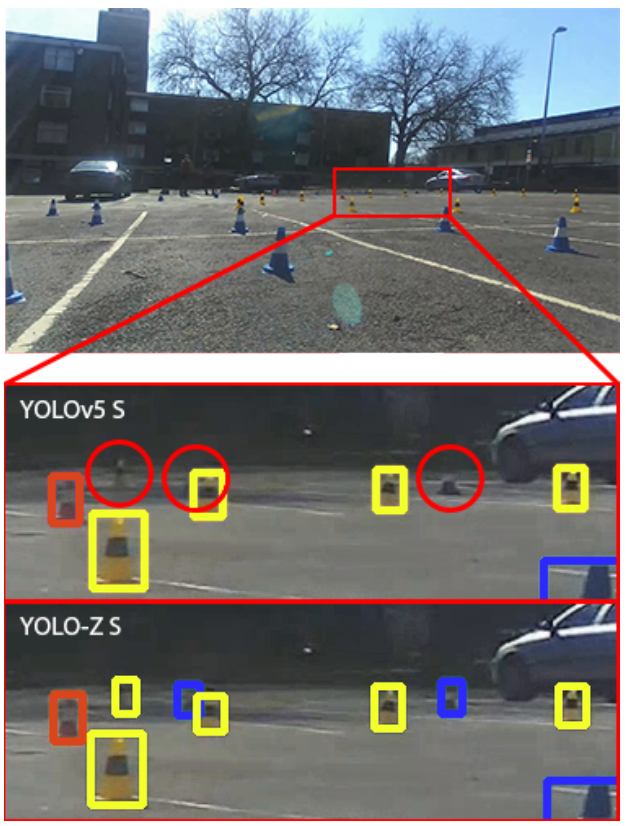
\includegraphics[width=.7\textwidth]{figures/yoloz-result.png}
    \caption*{Source: \textcite{yoloz}}
    \caption{Small objects in the image. Comparison of YOLOZ-S and YOLOv5-S. YOLOv5-S was not able to detect the circled objects.}
    \label{fig:yolozcone}
  \end{figure}
  YOLO-Z is a derivative architecture of YOLOv5r5.0.
  This variant of YOLO modified the backbone, neck, and number of anchors of the original YOLOv5 to 
  enhance its capability of detecting small objects \parencite{yoloz}.
  These changes are backbone change from YOLOv5r5.0 to a downscaled DenseNet,
  neck change from FPN to biFPN on some YOLO-Z scales, and increasing the number of anchors used at each scale.

  YOLO-Z was aimed to be used in autonomous racing car. In this high speed environment, early detection
  of obstacle is crucial to plan for action. For that reason, the autonomous racing car must detect the cone-shaped obstacles
  that are far away from it. Since objects that are far away appear small on image captured by camera, YOLOv7 was designed with
  purpose of small object detection.
  %YOLO-Z merupakan arsitektur famili YOLO yang modifikasi dari YOLOv5 \parencite{yoloz}.
  %Modifikasi-modifikasi yang dilakukan meliputi pergantian \emph{backbone}, \emph{neck}, dan jumlah \emph{anchor}
  %\emph{Backbone} dari YOLOv5r5.0 menjadi DenseNet yang di-\emph{downscale}.
  %\emph{Neck} dari YOLO-Z juga diganti dari PanNet menjadi FPN dan biFPN tergatung pada \emph{scale} YOLO-Z yang digunakan.

  %Modifikasi pada YOLO-Z didesain untuk mendeteksi objek kecil untuk tujuan melakukan deteksi \emph{cone} yang nampak jauh pada lintasan \emph{autonomous racing} secara \emph{real time} (lihat Gambar \ref{fig:yolozcone}).
  %Modifikasi-modifikasi dibuktikan dapat meningkatkan kemampuan pendeteksian objek kecil \parencite{yoloz}.
  %Oleh karena itu, untuk meningkatkan kemampuan mendeteksi objek kecil YOLOv7, beberapa modifikasi yang dilakukan YOLO-Z pada YOLOv5 dapat diaplikasikan.

  \subsection{exYOLO}
  \begin{figure}[H]
    \centering
    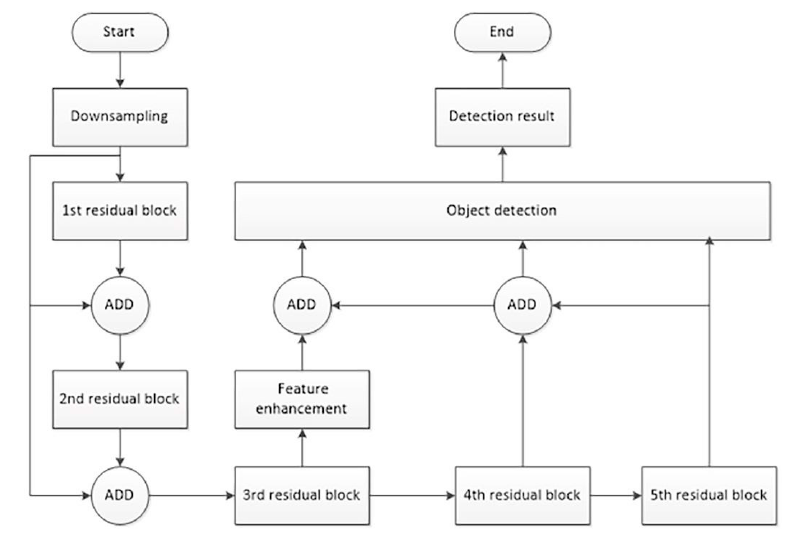
\includegraphics[width=0.8\textwidth]{figures/exyolo.png}
    \caption*{Source: \textcite{exyolo}}
    \caption{Architecture of exYOLO}
    \label{fig:exyolo}
  \end{figure}

  exYOLO is a modification of YOLOv3 to detect small objects \parencite{exyolo}.
  \textcite{exyolo} thought that the features of small objects in an image would disappear
  after series stage of down-sampling in the neural network.
  To solve this exYOLO added a feature enhancement before feature-fusion in the neck to one of the feature scale as seen in Figure \ref{fig:exyolo}.
  This change made exYOLO produce a higher mAP score on VOC2007 compared to its baseline YOLOv3.
    %exYOLO merupakan hasil modifikasi arsitektur YOLOv3 \parencite{exyolo}.
    %Pada exYOLO, dilakukan modifikasi \emph{neck} dengan menambahkan suatu \emph{Receptive Field Block} sebelum penggabungan \emph{feature map} yang akan diupsampling.
    %Modifikasi-modifikasi ini membuat exYOLO memiliki skor mAP yang lebih tinggi daripada YOLOv3 pada dataset PASCAL VOC 2007.

  \subsection{YOLOv4-tiny with added head}%Implementasi YOLOv4-tiny pada \emph{Autonomous Surface Vehicle}}
  \begin{figure}[H]
    \hfill%
    \begin{subfigure}[c][][c]{.45\textwidth}
        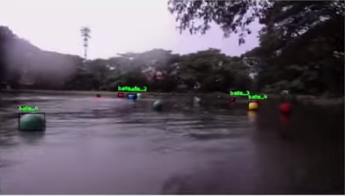
\includegraphics[width=1\linewidth]{figures/yolov4barun-regular.png}
        \caption{Regular YOLOv4-tiny prediction}
        \label{fig:barun-yolov4}
    \end{subfigure}\hfill  
    \begin{subfigure}[c][][c]{.45\textwidth}
        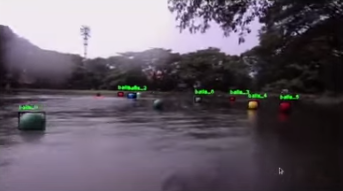
\includegraphics[width=1\linewidth]{figures/yolov4barun-addhead.png}
        \caption{YOLOv4-tiny with added head prediction}
        \label{fig:barun-yolov4-3l}
    \end{subfigure}\hfill%
    \caption*{Source: \textcite{barunastra}}
    \caption{Comparison of regular YOLOv4-tiny and YOLOv4-tiny with added head}
    \label{fig:barun}
  \end{figure}

  \textcite{barunastra} used YOLOv4-tiny as their Autonomous Surface Vehicle (ASV) object detector due to the computational
  device constraint.
  To detect objects that were atleast 30 meters away from the ASV, they applied a modification of YOLOv4-tiny, which was YOLOv4-tiny
  but with additional head layer. The original YOLOv4-tiny only had 2 head layers, thus was only predicting in 2 scales.
  An addition of head layer allows it to predict in 3 scales. Using this modification, the network was able to detect small object
  better and raised the overall mAP score by 4\% without significantly reducing latency.

  %\textcite{barunastra} menggunakan model modifikasi YOLOv4-tiny pada \emph{Autonomous Surface Vehicle}(ASV) mereka.
  %YOLOv4-tiny sebenarnya hanya menggunakan 2 layer head, namun yang diimplementasikan pada ASV adalah model YOLOv4-tiny
  %yang ditambahkan 1 layer head lagi sehingga menggunakan total sebanyak 3 layer head. Perubahan ini memberikan peningkatan
  %pada skor mAP dan memberikan kemampuan modelnya untuk mendeteksi objek yang lebih jauh.
\cleardoublepage

% contents 3 desain dan implementasi
\chapter{METHODS}
\section{Model Searching Method}
  %Untuk mencari solusi optimisasi pendeteksian objek kecil YOLOv7 yang terbaik, akan dilakukan penambahan atau perubahan \emph{bag-of-freebies}, \emph{bag-of-specials}, dan arsitektur YOLOv7.
  %Setiap modifikasi-modifikasi itu akan diaplikasikan secara independen dan kombinatif.
  %Yang dimaksud dengan kombinatif adalah modifikasi-modifikasi akan dikombinasikan menjadi 1 model YOLOv7.

  %Setiap kombinasi modifikasi, independen atau tidak, akan diuji kemampuannya mendeteksi objek \emph{airborne}.
  %Solusi optimisasi terbaik akan ditentukan berdasarkan metrik $AP_{50}$.
  %Subbab \ref{section:modificationcandidates} akan membahas tentang kandidat modifikasi-modifikasi yang dapat dilakukan.

  %Tahapan pencarian solusi optimisasi sendiri dapat dibagi menjadi enam tahap.
  %Tahap-tahap tersebut adalah Persiapan Dataset, Pembuatan \emph{Auto-trainer}, Pembuatan Konfigurasi Modifikasi, \emph{Training Model}, Analisis, dan Pemilihan Model Terbaik.
  %Urutan pengerjaan dari tahap-tahap ini dapat dilihat pada Gambar \ref{fig:metodologi}.
To find the best model for detecting small objects, trial and error will be performed by
adding or changing architecture, bag-of-specials, or bag-of-freebies of YOLOv7.
These modifications will be tried out independently and combinatively.

Every modification will be tested on its ability to detect airborne object.
The best model will be selected based on $mAP@50$ metric.
This metric was chosen instead of $mAP@[50:95]$ because we don't expect for the model to be able to predict a tightly fit
bounding boxes for small object and consider a loose 50\% coverage IoU is good enough.

The model searching method is comprised of six steps.
These steps are dataset preparation, develop training system, create modification model configuration,
training the model, analysis, and model selection. 
Figure \ref{fig:methods} shows the order these steps will be executed.

\begin{figure}[H]
  \centering
  \small
  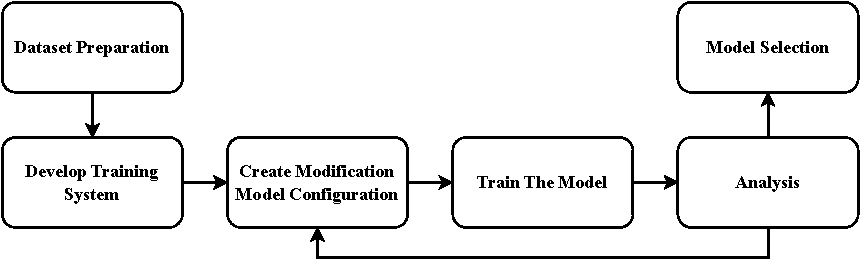
\includegraphics[width=.9\textwidth]{figures/methods.pdf}
  \caption{Search Steps}
  \label{fig:methods}
\end{figure}
\vspace{-1ex}
  %insert diagram modifikasi here
  %Menyiapkan dataset, Membuat \emph{auto-trainer}, Membuat konfigurasi-konfigurasi modifikasi, Melatih model-model YOLOv7 yang sudah dimodifikasi,
  %Menganalisis performa hasil modifikasi YOLOv7, dan Pemilihan model modifikasi YOLOv7 dengan skor mAP terbaik.

  %Pada tahap persiapan dataset, akan dilakukan pengunduhan dataset dari \textcite{aot_dataset}.
  %Gambar-gambar pada dataset ini kemudian akan di-\emph{sampling} dan didistribusikan menjadi dataset \emph{training}, validasi, dan pengujian.
  %Pada pendistribusian dataset ini juga akan dilakukan \emph{balancing} antar kelas dan dataset positif negatif.
  %\emph{Balancing} dilakukan agar tidak ada kelas yang mendominasi pada dataset.

  %Selanjutnya, di tahap pembuatan \emph{auto-trainer}, akan dilakukan pembuatan program yang dapat dengan otomatis membangun dan melatih \emph{neural network} modifikasi YOLOv7.
  %Pembuatan \emph{auto-trainer} ini dilakukan agar proses-proses pengerjaan tahapan-tahapan selanjutnya menjadi dapat dilakukan dengan lebih mudah.

  %Setelah itu, akan dilakukan pembuatan konfigurasi-konfigurasi modifikasi.
  %Konfigurasi modifikasi YOLOv7 akan dibuat agar dapat diinputkan pada \emph{auto-trainer}.
  %Konfigurasi modifikasi akan berisi kombinasi modifikasi-modifikasi yang ada pada subbab \ref{section:modificationcandidates}.

  %Tahapan selanjutnya adalah \emph{Training} model.
  %Pada tahap ini, konfigurasi-konfigurasi modifikasi pada tahapan sebelumnya akan dibangun dan kemudian dilatih.
  %Model akan dilatih \emph{from scratch}. Dengan kata lain, model tidak akan dilatih dengan menggunakan \emph{pre-trained weights}.
  %Hasil dari tahap ini adalah \emph{weights neural network} modifikasi YOLOv7, histori pelatihannya, dan metrik-metriknya pada dataset uji.

  %Pada tahap analisis, hasil dari tahap sebelumnya akan dianalisis untuk mencari tahu performa model-model hasil modifikasi.
  %Analisis juga dilakukan untuk menemukan \emph{gap} kandidat modifikasi lain yang masih bisa dieksplorasi untuk meningkatkan kemampuan pendeteksian objek kecil YOLOv7.
  %Ketika suatu kandidat modifikasi seperti itu ditemukan, maka akan dilakukan kembali pembuatan konfigurasi modifikasi untuk menguji kandidat modifikasi baru tersebut.

To conduct this research, we first have to prepare the dataset.
First, the dataset will be downloaded from \textcite{aot_dataset}.
Then, the labels of the dataset will be converted to darknet or COCO format.
Next, the dataset will be sampled into training set, validation set, and test set.
The sampling will be done in a way that balances the number classes in each set so
that there will be no dominating class during training.
  
The next thing to do is to develop a training system.
The purpose of this system is to make the training process easily conducted and monitored.
This system will include features such as train fail notification, train queueing, and alert the user
when the computer overheats.

Moving on, we have model configuration creation. Here we will create a model configuration file based on the 
modification that we want to try. The modification configurations will be made according to the modification
candidates listed in section \ref{section:modificationcandidates}.

The next step is to train the model.
The model configurations that was made in previous step will be built and trained from scratch (no pre-trained weights).
In this step, the weights of the neural network, training history, and performance metrics will be generated for analysis.

In the analysis step, we will analyze the performance of the modified YOLOv7.
This step is done to find other candidate of modification that might work.
If such modification candidate was found, we will go back to create the model configuration, 
and then train the modification.

Finally, in the last step we will select the best model.
We will select the model with the best performance among the modified YOLOv7 models.
The model selection will be done based on $mAP@50$ metric, with constraint in inference latency.
The model that qualify for selection must be able to perform inference with speed of atleast 10 FPS in a consumer GPU Nvidia RTX 2080Ti.
  %Tahapan terakhir adalah pemilihan model terbaik.
  %Pada tahapan ini akan dipilih model yang memiliki performa terbaik dari antara model-model hasil modifikasi lainnya.
  %Pemilihan model akan dilakukan dengan berdasarkan pada skor mAP tertinggi.
  %Untuk mempertahankan solusi optimisasi yang dapat melakukan deteksi secara \emph{real time}, model yang akan dipilih adalah model yang dapat melakukan deteksi yang cukup cepat pada \emph{edge} GPU.


\section{Modification Candidates}
\label{section:modificationcandidates}
  \subsection{Mosaic Augmentation}
  As discussed in section \ref{section:mosaic_study}, mosaic augmentation was able to increase the detection accuracy of small objects
  on many object detection neural networks. For this reason, we will experiment by training YOLOv7 with and without  mosaic augmentation.
    %Seperti yang dibahas pada subbab \ref{section:mosaic_study}, augmentasi mosaic pada dataset mampu meningkatkan akurasi deteksi objek-objek kecil dari model.
    %Oleh karena itu, akan dilakukan eksperimen menambahkan augmentasi mosaik pada YOLOv7 untuk melihat apakah augmentasi ini akan meningkatkan akurasi, khususnya pada dataset objek kecil.
  \subsection{Pre-training Anchor Recalculation}
    %Yang dimaksud dengan rekalkulasi \emph{anchor on-training}  adalah ketika ukuran-ukuran \emph{anchor box} direkalkulasi pada saat training.
    %Berbeda dengan \emph{clustering pre-training} seperti pada YOLOv2 \parencite{yolov2}, ukuran-ukuran \emph{anchor} akan di-\emph{learning} bersama dengan pendeteksi objeknya.
    %Untuk melakukan hal ini, digunakan algoritma optimisasi \emph{anchor box} yang mirip dengan algoritma \textcite{anchoropt}.
    %Pada bagian \emph{head}, akan ditempelkan suatu layer yang akan mengoutputkan faktor \emph{rescaling} dari tiap \emph{anchor box}.
    %Bagian tersebut akan di-\emph{training} bersama dengan YOLOv7 \emph{anchor box} akan teroptimisasi tidak hanya pada dataset, namun pada keseluruhan \emph{neural network} juga.

    %Anchor yang disediakan pada kode implementasi dari YOLOv7 merupakan anchor yang dikalkulasi untuk mengoptimisasi deteksi pada dataset
    %COCO2017. Dengan pertimbangan bahwa distribusi dataset yang akan digunakan pada penelitian ini berbeda dari objek general di COCO2017,
    %maka anchor harus direkalkulasi. Dengan melakukan rekalkulasi anchor, tiap layer head pada YOLOv7 akan dengan lebih mudah mem-\emph{fit}
    %objek-objek yang ada pada gambar.
  In the implementation code of YOLOv7, the anchors provided was calculated based on COCO2017 dataset.
  We assume that the dataset distribution of airborne objects to be greatly different from COCO2017.
  As such, the anchors must be recalculated for faster learning. This recalculation will be conducted
  using k-means algorithm. One problem however is that k-means might fail to cluster the dataset into 
  the amount of anchors that we needed. To tackle this, we might have to cluster it in logarithmic coordinates. 

  \subsection{Replacing Localization Loss to Extended IoU}
  \begin{figure}[H]
      \centering
      \begin{subfigure}[][][t]{0.3\textwidth}
        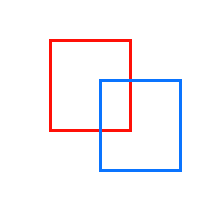
\includegraphics[width=1\linewidth]{figures/iounot0.png}
        \caption{$IoU > 0$ when 2 boxes intersect}
        \label{fig:iouexist}
      \end{subfigure}\hfill
      \begin{subfigure}[][][t]{0.3\textwidth}
        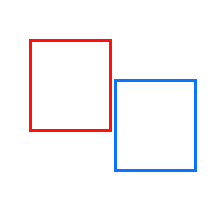
\includegraphics[width=1\linewidth]{figures/iou0near.png}
        \caption{$IoU = 0$ when 2 boxes does not intersect}
        \label{fig:iou0near}
      \end{subfigure}\hfill
      \begin{subfigure}[][][t]{0.3\textwidth}
        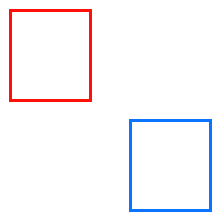
\includegraphics[width=1\linewidth]{figures/iou0far.png}
        \caption{$IoU = 0$ when 2 boxes does not intersect and far away}
        \label{fig:iou0far}
      \end{subfigure}
      \caption{Cause of IoU vanishing gradient}
      \label{fig:iouvanishinggrad}
  \end{figure}
  Extended-IoU (EIoU) is a modification of IoU that are used in neural networks to tackle
  the problem of vanishing gradient \parencite{eiou}. 
  IoU are known to cause vanishing gradient problem due to its behavior when two bounding boxes are not intersecting.
  When 2 boxes $A$ and $B$ are not intersecting, the area of intersection ($A\cap B$) would always be 0.
  This value doesn't give any information whether the boxes are far apart (Figure \ref{fig:iou0far}) or 
  near but not intersecting (Figure \ref{fig:iou0near}).
  To solve this, loss involving $IoU$ are usually paired with some regularization terms.
  For example \textcites{giou}{diou_ciou} proposed $GIoU$, $DIoU$, and $CIoU$.
  
  YOLOv7 itself is using $CIoU$ for its localization loss. $CIoU$ is just regular $IoU$
  that is paired with distance and box aspect ratio regularization terms.
  The problem of these kinds of regularized IoU is that when the boxes intersect, it does not
  behave like IoU anymore. $GIoU$, $DIoU$ and $CIoU$ have residue of their regularization when
  the boxes intersect. Metrics used to evaluate object detection
  algorithms depend on IoU (\textit{e.g.\ mAP}).
  For this reason \textcite{eiou} designed EIoU. The main appeal of EIoU
  is that it behave exactly like IoU when the boxes intersect and gives non-positive value when the
  boxes do not intersect.
  By behaving exactly like IoU, it is hoped that the model would perform better on the metrics.


    %\emph{Extended} IoU (EIoU) merupakan salahsatu modifikasi dari
    %IoU yang dibuat untuk menyelesaikan permasalahan \emph{vanishing gradient}
    %pada IoU \parencite{eiou}. Hal yang menyebabkan IoU bermasalah dengan \emph{vanishing gradient}
    %adalah nilai dari IoU yang selalu menjadi 0 ketika 2 \emph{bounding box} tidak beririsan.
    %Permasalahan ini diselesaikan oleh EIoU dengan memberikan nilai negatif untuk 
    %bounding box yang tidak beririsan, sehingga neural network dapat mengoptimasi loss function $-EIoU$.
    %Teknik konveksikasi juga dapat dilakukan dengan mengoptimasi $(1-EIoU)^2$

    %YOLOv7 sendiri menggunakan CIoU sebagai localization loss. CIoU juga merupakan suatu solusi
    %dari permasalahan \emph{vanishing gradient}. CIoU menambahkan suku jarak antar bounding box 
    %dan kecocokan \emph{aspect ratio} antar boundingbox pada IoU. Keunggulan EIoU daripada CIoU
    %adalah EIoU akan bertingkah seperti IoU ketika bounding box beririsan. Karena metrik-metrik
    %yang digunakan untuk mengukur kemampuan deteksi dilakukan berdasarkan IoU, dianggap akan
    %lebih baik jika loss yang digunakan sama seperti metriknya \parencite{eiou}.

  \subsection{Utilizing Earlier Feature Map Stage}
    %\begin{figure}[ht]
    %  \centering
    %  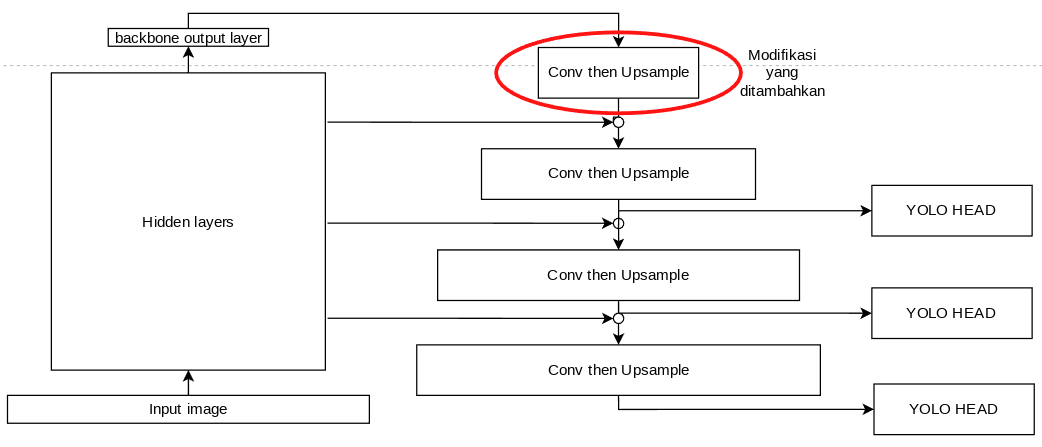
\includegraphics[scale=0.5]{figures/add-more-upsampling.png}
    %  \caption{Menambah \emph{upsampling} pada \emph{neck}}
    %  \label{fig:neckaddupsampling}
    %\end{figure}

  \begin{figure}[H]
    \centering
    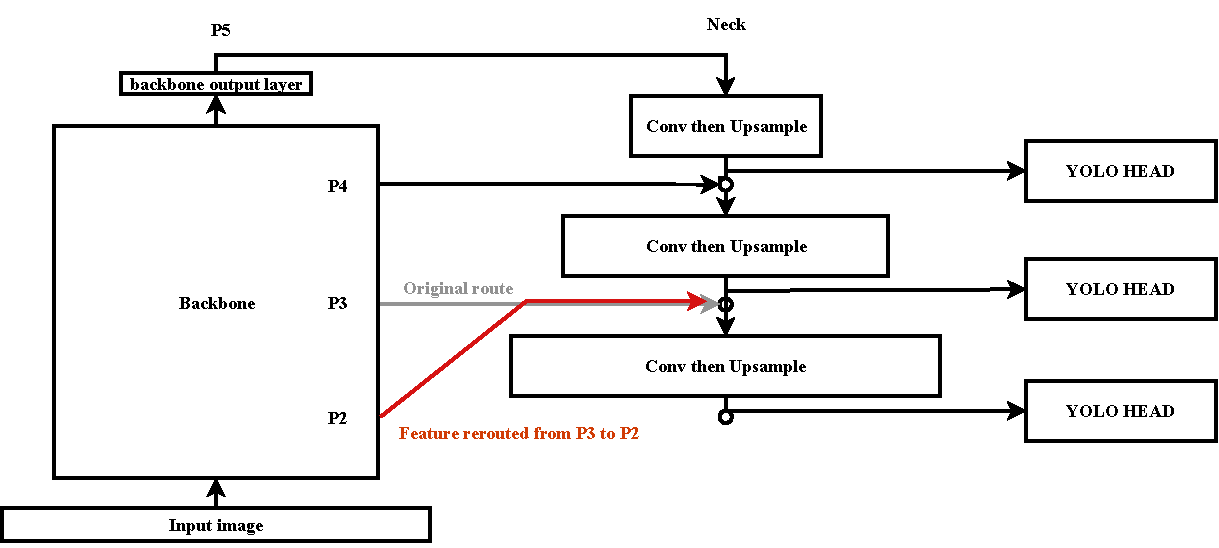
\includegraphics[width=.9\textwidth]{figures/neck-move-back.pdf}
    \caption{Rerouting Neck Connection to Earlier Stage}
    \label{fig:neckmoveback}
  \end{figure}
  In a deep neural network, the extracted feature/abstraction of the data become more prominent
  as the input data passes through deeper layers. However, information loss also increases in the
  deeper layer. For small object detection, information is crucial. There is a posibility the features
  of small objects are lost as the data propagates through the network.
  
  If we view it in a data path network design perspective, the greater the length of the path from input
  to output, the more information will be lost. Therefore, we propose to reroute the orignal connection from
  backbone to the neck to an earlier stage of inference. For example, YOLOv7 take feature maps from P3, P4, and P5
  scales of the backbone, we can reroute the connection from P3 to P2 as shown in Figure \ref{fig:neckmoveback}.
  %Seperti pada penelitian-penelitian terkait di subbab \ref{section:relatedwork}, modifikasi \emph{neck} dapat dilakukan untuk meningkatkan akurasi pendeteksian objek kecil.
  %Modifikasi koneksi \emph{neck} ke \emph{backbone} dapat dilakukan dengan memindahkan sumber feature map untuk beberapa layer neck lebih jauh ke belakang seperti pada Gambar \ref{fig:neckmoveback}.
  %%Penambahan layer upsampling dapat membuat neural network untuk mendapatkan feature-map yang lebih detail sehingga dapat melakukan pendeteksian objek kecil dengan lebih baik.
  %Pemindahan sumber feature map ke belakang dapat dilakukan untuk mengantisipasi fitur objek kecil yang bisa saja hilang ketika layer neural network semakin dalam.
  %Dengan memindahkannya lebih ke belakang, YOLOv7 akan melakukan deteksi dengan memanfaatkan fitur yang abstraksi yang lebih rendah tetapi sedikit informasi yang hilang.
  \subsection{Additional YOLO Head}
  \begin{figure}[H]
    \centering
    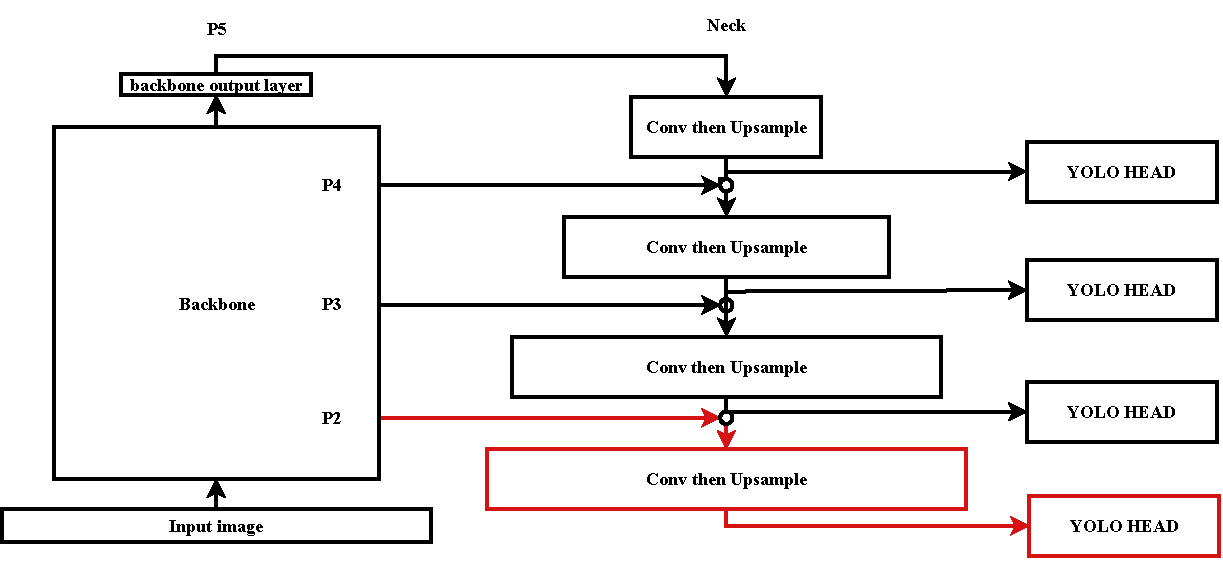
\includegraphics[width=.9\textwidth]{figures/addmorehead.pdf}
    \caption{Adding an Extra Head Layer}
    \label{fig:addmorehead}
  \end{figure}
  An additional YOLO head means an extra stage of detection.
  With more stage of detection, the large variance of the objects in the dataset can be learned.
  This is especially good for \textcite{aot_dataset} where the area of the bounding boxes in the dataset
  can be orders of magnitude apart (see section \ref{section:dataset}).
  
  %%Penambahan YOLO head dapat membuat YOLOv7 melakukan deteksi pada skala yang lebih banyak.
  %%Hal ini akan berpengaruh pada kemampuan pendeteksian objek kecil.
  %%Dengan melakukan pendeteksian pada skala yang lebih banyak, YOLOv7 dapat mendeteksi objek yang besar maupun kecil.
  %Perhatikan bahwa penambahan YOLO Head akan diikuti dengan penambahan \emph{layer upsampling} pada \emph{neck} seperti di Gambar \ref{fig:addmorehead}.

  \subsection{Replace YOLO Head to YOLOX's Decoupled Anchor-free Head}
  \begin{figure}[H]
    \centering
    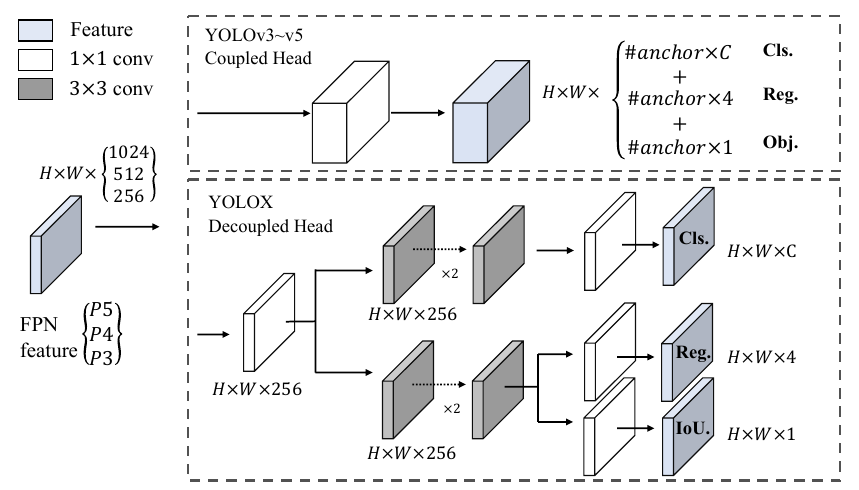
\includegraphics[width=0.8\textwidth]{figures/anchorfree-yolox.png}
    \caption{Decoupled Anchor-free Head in YOLOX compared to Coupled Head in mainstream YOLO}
    \label{fig:anchorfree}
  \end{figure}

  YOLOv6 and YOLOX used a different kind of head layer compared to usual YOLO \parencites{yolox}{yolov6}. 
  In mainstream YOLO, prediction for bounding box and classes are both calculated on the same layer.
  With decoupled anchor-free head, the layers are separated for class prediction and bounding box prediction, and
  bounding box prediction are done using 4 value without anchor as seen on Figure \ref{fig:anchorfree}. 
  Using decoupled anchor-free head gives us 2 advantages. 1) Reducing the amount of design parameters as 
  we don't have to introduce anchor boxes to the model. 2) Reducing the complexity of interpreting prediction
  result. Advantage (1) is especially enticing. There is a possibility of us introducing bad priors to the neural
  network by poorly clustering anchor boxes. By having a model that less dependent on prior, we can reduce such possibility.

  A thing to consider when applying decoupled anchor-free head to YOLOv7 is the label assigner. YOLOv7 and YOLOX uses SimOTA as its default
  label assigner. However, \textcite{yolov6} YOLOv6 uses Task-aligned Assigner (TAL) for its label assigner. They reported that TAL performs
  better than SimOTA. Therefore, in applying decoupled anchor-free head, it might be better to use TAL as label assigner.
  %Decoupled head gives us 2 advantages. 
  %1) Reducing the amount of


  %Pada YOLOX, \emph{coupled anchor head} seperti pada arsitektur YOLO pada umumnya diganti dengan \emph{decoupled anchor-free head} \parencite{yolox}.
  %Keuntungan dari model anchor-free adalah kita tidak perlu mendefinisikan \emph{anchor} sebelum melakukan training sehingga mengurangi beberapa proses
  %tuning heuristik seperti rekalkulasi anchor. Memakai \emph{head} yang anchor free juga memberi kompleksitas proses training dan pendekodean output model.
  %\cite{yolox} melaporkan peningkatan pada akurasi dan pengurangan parameter sehingga mempercepat lama deteksi.
  %Oleh karena hal-hal tersebut, mencoba memakai \emph{head anchor-free} di YOLOv7 baik untuk dicoba.
    
    
\section{Dataset}
\label{section:dataset}

  \subsection{Source}
  \label{section:datasetsource}
  Dataset containing annotated images of airborne objects can be obtained from \textcite{aot_dataset}.
  This dataset is hosted in an AWS S3 Bucket.
  The dataset consist of several Unmanned Aerial Vehicle (UAV) flights' frame-by-frame camera capture.
  There are 7 classes in the dataset but most there are 3 dominating classes.
  The size of the dataset and its class distribution can be seen on Figure \ref{tbl:datasettraintest} and
  \ref{tbl:datasetclasses} respectively.
  %Dataset untuk objek-objek \emph{airborne} didapatkan dari \textcite{aot_dataset} dan dihost pada suatu server AWS S3 Bucket.
  %Dataset ini berisi video-video monokromatik penerbangan UAV.
  %Terdapat 4 kelas pada dataset ini yaitu pesawat, helikopter, burung, dan \emph{other}.
  %Distribusi dataset training dan uji dapat dilihat pada tabel \ref{tbl:datasettraintest} sedangkan distribusi kelas dari dataset dapat dilihat pada Tabel \ref{tbl:datasetclasses}.
  \begin{table}[H]
    \centering
    \captionof{table}{Original Dataset Splits}
    \label{tbl:datasettraintest}
    
\begin{table}[H]
  \centering
  \captionof{table}{Distribusi Dataset Training dan Test}
  \label{tbl:datasettraintest}
  \begin{tabular}{|c|c|c|c|c|}
    \hline
    Pembagian & Ukuran (TB) & Sekuen penerbangan & Jumlah Gambar & Jumlah Label\\
    Dataset &  & UAV &  & \\
    \hline
    Training & 11,3 & 4154 & 4975765 & 2891891\\
    \hline
    Validation + Test &2.1 &789 & 943852 & 496075\\
    \hline
    Total &13,4 &4943 & 5919617 & 3387966\\
    \hline
  \end{tabular}
\end{table}
  \end{table}
  \begin{table}[H]
    \centering
    \captionof{table}{Dataset' Objects Classes Distribution}
    \label{tbl:datasetclasses}
    \begin{tabular}{ c c c c c c }
  \toprule[1.5pt]
  Splits & Total Objects & Airplane & Helicopter & Bird & \emph{Other 4 Classes}\\
  \midrule
  Training & 2,89 M & 0,79 M& 1,22 M& 0,33 M& 0,54 M\\
  Validation + Test &0,50 M &0,13 M & 0,17 M&0,06 M&0,14 M\\
  \midrule
  Total &3,39 M &0,92 M & 1,39 M&0,39 M&0,69 M\\
  \bottomrule[1.5pt]
\end{tabular}
  \end{table}
  %Kebanyakan \emph{bounding box} pada dataset berukuran sangat kecil.
  %Distribusi dari luas \emph{boudning box} dapat dilihat pada gambar \ref{fig:areadist}.
  %Perhatikan pada gambar tersebut, sumbu x menggunakan skala logaritmik.
  %Sebagai referensi, luas dari tiap frame itu sekitar $5\times10^16 px^2$.
  %\begin{figure}[H]
  %  \centering
  %  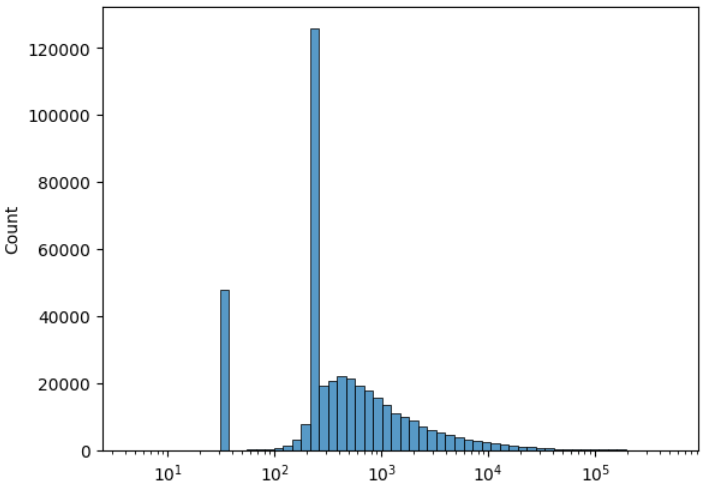
\includegraphics[scale=0.65]{figures/area-dist.png}
  %  \caption{Penambahan \emph{Layer} Head pada YOLO}
  %  \label{fig:areadist}
  %\end{figure}

  
  \subsection{Sampling Dataset}
  As seen on section \ref{section:datasetsource}, The size of the dataset is massive.
  Due to the limitation of computational resource, we will only able to sample some of them
  for training and testing. We will sample in total 700 images from the dataset with splits
  as shown in Table \ref{tbl:datasetsamplingdist}.
  %Karena jumlah dataset pada \textcite{aot_dataset} berukuran sangat besar, dan keterbatasan
  %\emph{computational resource}, hanya sebagian dari dataset tersebut akan digunakan untuk \emph{training} dan \emph{test}.
  %Akan diambil total 700 gambar dari dataset dengan pembagian sesuai dengan Tabel \ref{tbl:datasetsamplingdist}
  \begin{table}[H]
    \centering
    \captionof{table}{Distribusi Sampling Dataset}
    \label{tbl:datasetsamplingdist}
    \begin{tabular}{c c c c c c c}
      \toprule[1.5pt]
      Splits    &Total &\multicolumn{5}{c}{Classes Percentage}\\
                        \cline{3-7}
                &Images& Airplane & Helicopter & Bird & Drone & Negative\\
      \midrule
      Training  &400   &23.75\%   &23.75\%     &23.75\% &23.75\%       &5\%\\
      \midrule
      Validation&100   &20\%      &20\%        &20\%    &20\%          &20\%\\
      \midrule
      Test      &200   &20\%      &20\%        &20\%    &20\%          &20\%\\
      \bottomrule[1.5pt]
    \end{tabular}
  \end{table}

  %Untuk membagi dataset agar terdistribusi seperti pada Tabel \ref{tbl:datasetsamplingdist}, akan digunakan algoritma seperti berikut:
  %\begin{algorithmic}
  %  \State $L_0 \gets$ List index gambar-gambar yang memiliki objek kelas pesawat
  %  \State $L_1 \gets$ List index gambar-gambar yang memiliki objek kelas helikopter
  %  \State $L_2 \gets$ List index gambar-gambar yang memiliki objek kelas burung 
  %  \State $L_3 \gets$ List index gambar-gambar yang memiliki objek kelas \emph{Other}
  %  \State $L_4 \gets$ List index gambar-gambar yang memiliki objek kelas negatif
  %  \For{$i \gets 0$ to $4$}
  %    \State $L_i \gets shuffle(L_i)$
  %  
  %  

  %\end{algorithmic}

\section{Instruments}
To conduct this research, we will be using a computer with the following specs:
\begin{itemize}[noitemsep,topsep=0pt,leftmargin=.1\textwidth,rightmargin=.1\textwidth]
  \item CPU \hfill Intel® Core™ i5-9400F CPU @ 2.90GHz
  \item GPU \hfill Nvidia Geforce RTX 2080 Ti
  \begin{itemize}[noitemsep,topsep=0pt]
    \item[] Memory \hfill 11 GB
    \item[] CUDA Compute Capability \hfill 7.5
  \end{itemize}
  \item RAM \hfill 12 GB
  \item Hard Drive Available Memory \hfill 1.3 TB
  \item Operating System \hfill Ubuntu 20.04
  \item Cuda Toolkit Version \hfill 11.7
  \item PyTorch Version \hfill 1.13.1
\end{itemize}
%\begin{tabular}{>{\hspace{1em}}l >{\hspace{1pt}}l >{\hspace{3em}}l}
  CPU &       & Intel® Core™ i5-9400F CPU @ 2.90GHz\\
  GPU &       & Nvidia Geforce RTX 2080 Ti\\
      &Memory & 12 GB\\
      &Cuda CC& 7.5\\
  RAM &       & 12 GB\\

\end{tabular}

%\begin{itemize}[noitemsep,topsep=0pt]
%  \item CPU \hfill Intel(R) Core(TM) i5-9400F CPU @ 2.90GHz
%  \item GPU \hfill Nvidia Geforce RTX 2080 Ti
%  \begin{itemize}[noitemsep,topsep=0pt]
%    \item[] Memory \hfill 12 GB
%    \item[] CUDA Compute Capability \hfill 7.5
%  \end{itemize}
%  \item RAM \hfill 12 GB
%  \item Disk Available Memory \hfill 1.3 TB
%  \item Operating System \hfill Ubuntu 20.04
%  \item Cuda Toolkit Version \hfill 11.7
%  \item PyTorch Version \hfill 1.13.1
%\
  %Untuk melaksanakan eksperimen ini, akan digunakan suatu komputer yang dilengkapi dengan
  %GPU Nvidia RTX 2080 Ti yang memiliki kapasitas 11GB VRAM. Oleh karena keterbatasan ini,
  %Melatih model-model YOLOv7 besar seperti W6, E6, dan E2E yang dimodifikasi menjadi sangat sulit,
  %apalagi pada skala input sesuai dengan dimensi dataset.
  %Oleh karena hal ini, arsitektur yang akan dipilih sebagai \emph{baseline} modifikasi adalah YOLOv7 dengan
  %ukuran normal karena model tersebut adalah model terbesar yang mampu di-\emph{train} pada RTX 2080 Ti dengan 
  %input size 1600x1600 dan batch size 1.

  %Selain itu, jumlah dataset yang akan digunakan juga akan dibatasi menjadi 400 seperti pada subbab \ref{section:dataset} untuk menghemat waktu training.
  %Pada pilot test, ditemukan bahwa dibutuhkan sekitar 20 jam untuk men-\emph{train} model sebanyak 300 epoch pada dataset dengan 400 gambar jika menggunakan
  %GPU RTX 2080 Ti.





%\section{Skema Training Model}
%  Untuk melatih berbagai modifikasi YOLOv7, akan dibuat suatu \emph{auto-trainer}.
%  \emph{Auto-trainer} ini akan menerima suatu \emph{file} konfigurasi modifikasi YOLOv7, dan dengan otomatis membangun arsitektur YOLOv7 yang termodifikasi dan melatihnya.
%  Setelah mendapatkan model modifikasi YOLOv7 yang sudah dilatih, \emph{auto-trainer} akan menguji model tersebut dengan dataset uji.
%  Metrik-metrik pengujian, grafik histori \emph{training loss vs validation loss}, dan \emph{weights} dari model kemudian akan dikirim ke user.
%  Dengan membuat \emph{auto-trainer} ini, proses pelatihan model dan pelaporan hasil menjadi terotomasi sehingga akan mempermudah proses penelitian.
%
%\section{Timeline Pelaksanaan Penelitian}
%  \newcommand{\w}{}
%  \newcommand{\G}{\cellcolor{gray}}
%  \begin{table}[h!]
%    \captionof{table}{Tabel timeline}
%    \label{tbl:timeline}
%    \begin{tabular}{|p{3.5cm}|c|c|c|c|c|c|c|c|c|c|c|c|c|c|c|c|}
%  
%      \hline
%      \multirow{2}{*}{Kegiatan} & \multicolumn{16}{|c|}{Minggu} \\
%      \cline{2-17} &
%      1 & 2 & 3 & 4 & 5 & 6 & 7 & 8 & 9 & 10 & 11 & 12 & 13 & 14 & 15 & 16 \\
%      \hline
%  
%      % Gunakan \G untuk mengisi sel dan \w untuk mengosongkan sel
%      Persiapan Dataset &
%      \G & \w & \w & \w & \w & \w & \w & \w & \w & \w & \w & \w & \w & \w & \w & \w \\
%      \hline
%  
%      Pemb. \emph{Auto-trainer} &
%      \w & \G & \w & \w & \w & \w & \w & \w & \w & \w & \w & \w & \w & \w & \w & \w \\
%      \hline
%  
%      Pemb. Konfigurasi&
%      \w & \w & \G & \G & \G & \G & \G & \G & \G & \G & \G & \G & \w & \w & \w & \w \\
%      Modifikasi &
%      \w & \w & \G & \G & \G & \G & \G & \G & \G & \G & \G & \G & \w & \w & \w & \w \\
%      \hline
%  
%      Training Model &
%      \w & \w & \G & \G & \G & \G & \G & \G & \G & \G & \G & \G & \w & \w & \w & \w \\
%      \hline
%
%      Analisis &
%      \w & \w & \G & \G & \G & \G & \G & \G & \G & \G & \G & \G & \G & \w & \w & \w \\
%      \hline
%
%      Pemb. Laporan &
%      \w & \w & \w & \w & \w & \w & \w & \w & \w & \w & \w & \w & \G & \G & \G & \G \\
%      \hline
%  
%    \end{tabular}
%  \end{table}

\cleardoublepage

% contents 4 pengujian dan analisis
\chapter{EXPERIMENTS}

% Ubah bagian-bagian berikut dengan isi dari pengujian dan analisis

%Pada bab ini, akan dipaparkan pengaruh modifikasi-modifikasi yang dilakukan pada YOLOv7.
\section{Baseline Performance}
For comparison purposes, we first measure the baseline performance of YOLOv7 with all
modification candidates from section \ref{section:modificationcandidates} stripped.
We call this model as \verb|YOLOv7-plain|.
After 300 epochs of training with batch-size 1 like in the experiment setup, we found that
this model was unable to detect anything on the test set (a valid detection is detection with $IoU>0.5$ to groundtruth). 
%Untuk mengukur pengaruh dari modifikasi-modifikasi yang dilakukan pada YOLOv7, maka
%hal pertama yang harus dilakukan adalah mengukur performa YOLOv7 tanpa segala modifikasi
%yang diajukan pada bab \ref{section:modificationcandidates}. Arsitektur YOLOv7 \emph{plain} 
%ini di-\emph{train} pada 400 sampel data dari  \textcite{aot_dataset} dengan 300 epoch dan batch size 1.
%Dengan aturan tersebut, ditemukan bahwa model \emph{plain} tidak mampu untuk mendeteksi
%objek apapun pada dataset uji, dengan kriteria "terdeteksi" $IoU > 0.5$ (mAP@.5 = 0).
%
%Untuk keperluan komparasi dengan performa-performa dari modifikasi pada YOLOv7,
%model \emph{plain} ini akan selanjutnya disebut sebagai \verb*|YOLOv7-plain|.

\section{Mosaic Augmentation and Anchor Recalculation}


%Terdapat 3 modifikasi yang diujikan pada bagian ini, yaitu \verb*|YOLOv7-plain| yang ditambahkan augmentasi mosaic,
%\verb*|YOLOv7-plain| yang direkalkulasi anchor, dan \verb*|YOLOv7-plain| yang ditambahkan augmentasi mosaic dan rekalkulasi anchor.
In this section, we present the effect of mosaic augmentation and anchor recalulation on the $mAP@50$ score when applied
independently and combinatively. For comparison purposes, we assigned names the models as \verb|YOLOv7-M|,
\verb|YOLOv7-AR|, and \verb|YOLOv7-MAR|. These names correspond to \verb|YOLOv7-plain| with mosaic augmentation, \verb|YOLOv7-plain|
with anchor recalculation, and \verb|YOLOv7-plain| with both mosaic augmentation and anchor recalculation, respectively.
%\subsection{Augmentasi Mosaic}

The process of applying mosaic augmentation to the dataset is pretty straightforward as YOLOv7's implementation code
already provide the mosaic augmentation tool. A mosaic augmentation result example can be seen in Figure \ref{fig:mosaic-train}.
  %Proses melakukan augmentasi mosaic cukup \emph{straightforward},
  %augmentasi ini dilakukan pada beberapa data training.
  %Contoh hasil augmentasi dapat dilihat pada gambar \ref{fig:mosaic-train}
  \begin{figure}
    \centering
    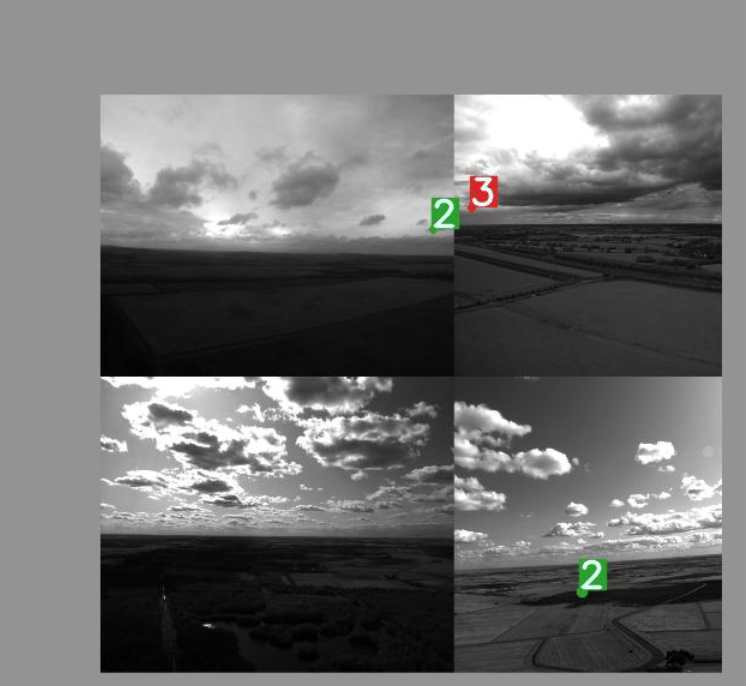
\includegraphics[scale=0.4]{figures/mosaic-aug-2.png}
    \caption{An example of mosaic augmented image}
    \label{fig:mosaic-train}
  \end{figure}

  %, sedangkan untuk rekalkulasi anchor akan dibahas pada bagian berikut.
%\subsection{Rekalkulasi Anchor}
%Rekalkulasi anchor dilakukan dengan mengklaster data training ke 9 centroid menggunakan algoritma k-means.
Anchor recalculation is done by clustering the training data's widths and heights to 9 centroid using k-means algorithm.
However, due to the skewed distribution of the dataset, regular k-means (with $L^2$ Distance) actually failed to form 9 clusters.
To fix this, we used a distance function
\begin{equation} 
  L = \sqrt{\ln^2{\frac{w_1}{w_2}} + \ln^2{\frac{h_1}{h_2}}}
  \label{eq:logdistancefunc}
\end{equation}
Distance function in equation \ref{eq:logdistancefunc} was actually an $L^2$ distance but with log-transformed space.
With this function, k-means was finally able to cluster the data into 9 centroids.
These centroids are used by the head layers as anchors. Each head uses 3.
The comparison of the original anchor and recalculated anchor can be seen in Table \ref{tbl:recalculated_anchor}
and Figure \ref{fig:anchor-dist}.
%Sembilan centroid tersebut digunakan sebagai anchor, 3 untuk tiap head pada arsitektur YOLO (terdapat 3 head).
%Persebaran anchor sebelum dan sesudah direkalkulasi dapat dilihat 
%pada Tabel \ref{tbl:recalculated_anchor} dan Gambar \ref{fig:anchor-dist}

\begin{table}
  \centering
  \captionof{table}{Anchor Points Before and After Recalculation}
  \label{tbl:recalculated_anchor}
  \vspace{-1ex}
  \begin{table}[H]
  \centering
  \captionof{table}{Titik Hasil Rekalkulasi Anchor}
  \label{tbl:recalculated_anchor}
  \vspace{-1ex}
  \begin{tabular}{ c l l }
    \toprule[1.5pt]
    Layer Head & Anchor Lama        & Hasil Rekalkulasi Anchor\\
    \midrule
    1          & [12,16], [19,36], [40,28]& [4,4], [14,5], [11,11]\\
    2          & [36,75], [76,55], [72,146]& [27,8], [18,17], [41,14]\\
    3          & [142,110], [192,243], [459,401]& [43,32], [86,27], [149,70]\\
    \bottomrule[1.5pt]
  \end{tabular}
\end{table}
\end{table}
\vspace{1ex}

\begin{figure}
  \centering
  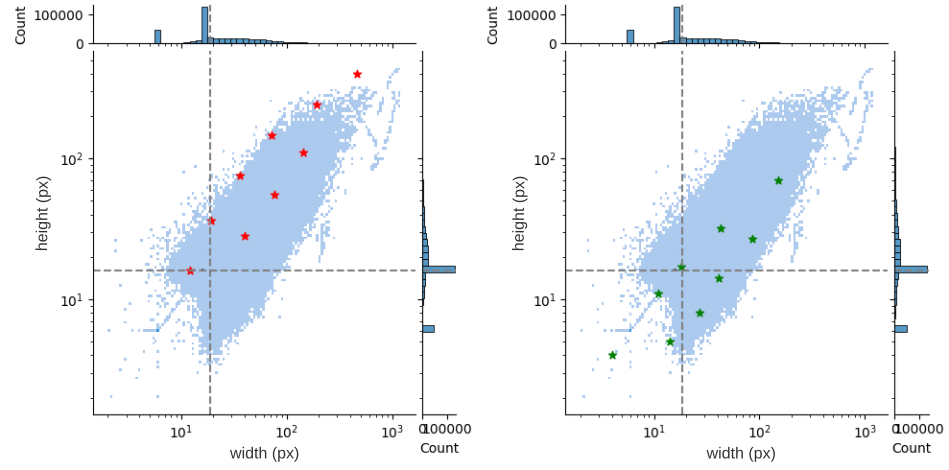
\includegraphics[width=\textwidth]{figures/anchor-dist-2.png}
  \caption{Anchor Distribution on Dataset. Left: Original Anchor. Right: Recalulated Anchors}
  \label{fig:anchor-dist}
\end{figure}

If we observe the distribution of anchors before and after recalculation in Figure \ref{fig:anchor-dist},
we can see that indeed the recalculated anchors cover more of the dataset than the original.
8 out of 9 of the original anchors are placed in the first quadrant of the median axis.
It means that those 8 anchors are responsible for only 25\% of the dataset and leave the rest to 1 anchor.
This is very inefficient. In contrast, the recalculated anchors have a more balanced distribution with
anchors distributed across each quadrant.


%Jika kita memperhatikan persebaran anchor sebelum dan sesudah direkalkulasi pada Gambar \ref{fig:anchor-dist},
%dapat kita lihat bahwa anchor hasil rekalkulasi lebih mencakup seluruh persebaran dataset daripada anchor lama.
%8 dari 9 anchor lama bertempat di kuadran pertama dari garis median(garis putus-putus).
%Hal ini berarti 8 anchor tersebut hanya mampu mendeteksi sekitar 25\% dari objek-objek pada dataset.
%Sedangkan, anchor hasil rekalkulasi menempatkan anchor di setiap kuadran.



\subsubsection{Performance}
%The performance of the 3 models compared to \verb|YOLOv7-plain| can be seen in Table \ref{tbl:mosaic_reanchor_performance}.
%We can see from the table that \verb|YOLOv7-plain| was only able to detect anything on the test set after applying both
%mosaic augmentation and anchor recalculation. With those 2 modification, the model was able to achieve 11.2\% score at mAP@50.
The performance of the three models, namely \verb|YOLOv7-M|, \verb|YOLOv7-AR|, and \verb|YOLOv7-MAR|, was compared to that of the baseline model YOLOv7-plain.
The results are presented in Table \ref{tbl:mosaic_reanchor_performance}.
It can be observed from the table that YOLOv7-plain alone was unable to detect any objects in the test set.
However, after applying both mosaic augmentation and anchor recalculation, the model achieved a notable improvement with a score of 11.2\% at mAP@50. 

\begin{table}
  \centering
  \captionof{table}{Mosaic Augmentation and Anchor Recalculation Performance}
  \label{tbl:mosaic_reanchor_performance}
  \vspace{-1ex}
    \begin{tabular}{ l l >{\hspace{4em}}c }
    \toprule[1.5pt]
    No & Model        &mAP@50 \\
    \midrule
    0  & \texttt{YOLOv7-plain}        & 0\%\\
    1  & \texttt{YOLOv7-M}            & 0\%\\
    2  & \texttt{YOLOv7-AR}           & 0\%\\
    3  & \texttt{\textbf{YOLOv7-MAR}} & \textbf{11.2}\%\\
    \midrule
       & Improvement                  & \textbf{\textcolor{green}{+11.2\%}}\\
    \bottomrule[1.5pt]
  \end{tabular}
\end{table}

Since the model \verb|YOLOv7-MAR| was the only model that was capable of detection in the test set,
we henceforth establish this model as the baseline for further modification. Meaning, in the subsequent
sections, any modifications mentioned should be presumed to be composed of mosaic augmentation and anchor recalculation,
in addition to the respective modification that was applied, unless explicitly stated otherwise.

  %Performa dari tiap modifikasi dapat dilihat pada tabel \ref{tbl:mosaic_reanchor_performance}.
  %Pada tabel tersebut, terlihat bahwa YOLOv7 mampu untuk mendeteksi beberapa objek pada dataset uji ketika diberi 
  %augmentasi mosaic pada data train dan direkalkulasi anchornya.
  %\begin{table}[H]
  \centering
  \captionof{table}{Performa Modifikasi Augmentasi Mosaic dan Rekalkulasi Anchor}
  \label{tbl:mosaic_reanchor_performance}
  \vspace{-1ex}
  \begin{tabular}{ l l c }
    \toprule[1.5pt]
    No & Modifikasi        &mAP@50 \\
    \midrule
    0  & \textbf{yolov7-plain               }& 0\%\\
    1  & \textbf{mosaic                     }& 0\%\\
    2  & \textbf{rekalkulasi anchor         }& 0\%\\
    3  & \textbf{mosaic + rekalkulasi anchor}& \textbf{11,2}\%\\
    \midrule
       & Peningkatan                         & \textbf{\textcolor{green}{+11,2\%}}\\
    \bottomrule[1.5pt]
  \end{tabular}
\end{table}

  %Hanya modifikasi nomor 3 yang mampu melakukan deteksi, maka 
  %modifikasi tersebut dijadikan baseline untuk modifikasi-modifikasi lainnya.
  %Untuk mempermudah komparasi penambahan modifikasi-modifikasi selanjutnya,
  %maka model ini akan disebut sebagai \verb*|YOLOv7-base|.

\section{Replacing Localization Loss to EIoU}
%Dengan menggunakan \verb*|YOLOv7-base| sebagai baseline, 
%Box Loss function dari YOLOv7 diganti menjadi EIoU.
%Telah juga dilakukan percobaan menggunakan convexciation pada EIoU.
%Hasil dari pengujian dapat dilihat pada Tabel \ref{tbl:loss_function_perf}
In this section, we experimented with $EIoU$.
We replaced the original $CIoU$ loss of YOLOv7 to pure $EIoU$ and convexcified version of $EIoU$.
The convexciation was done by modifying the $EIoU$ loss from $-EIoU$ to $(1-EIoU)^2$ for better
gradient dynamics during training.

The performance of these modifications can be seen in Table \ref{tbl:loss_function_perf}

\begin{table}[b]
  \centering
  \captionof{table}{EIoU Localization Loss Performance}
  \label{tbl:loss_function_perf}
  \vspace{-1ex}
    \begin{tabular}{ l l c }
    \toprule[1.5pt]
    No & Modification        &mAP@50 \\
    \midrule
    0  & \texttt{\textbf{YOLOv7-MAR +CIoU}} (original)     & \textbf{11.2}\%\\
    1  & \texttt{YOLOv7-MAR + EIoU}                & 0\%\\
    2  & \texttt{YOLOv7-MAR + EIoU + Convexication} & 4.92\%\\
    \midrule
       & Peningkatan                                & \textbf{\textcolor{red}{-6.28\%}}\\
    \bottomrule[1.5pt]
  \end{tabular}
\end{table}

Surprisingly, although $EIoU$ outperformed $CIoU$ when applied to networks like Faster-RCNN+ResNet and RetinaNet
as \textcite{eiou} claimed, it performed worse when applied to YOLOv7 with \textcite{aot_dataset}.
Even after convexciation, $CIoU$ still outperform $EIoU$ by 6.28\%.
%Ternyata, meskipun EIoU memiliki performa lebih baik daripada CIoU ketika diaplikasikan
%pada Faster-RCNN+ResNet50 dengan dataset VOC2007 dan COCO2017, EIoU tidak mampu untuk meningkatkan
%AP deteksi YOLOv7 pada dataset \textcite{aot_dataset}.

\section{Utilizing Earlier Feature Map Stage}
For this modification, we reconfigured the source of the feature map by redirecting it from P3 to P2, as shown in Figure \ref{fig:deeperconn}.
Specifically, we adjusted the routing on layer 66, changing it from 24 to 11. 
Since the output of layer 11 is at a different scale compared to 24 (with a scaling factor of $2^{-2}$ and $2^{-3}$ respectively), 
we modified the upsampling factor of layer 55 from 2 to 4 to ensure size compatibility with layer 11. 
However, this change in upsampling disrupted the subsequent layers. 
To solve this, we performed downsampling after layer 75 (connected to the head) by setting layer 77's stride to 2 and layer 79's stride to 4, 
resolving the size mismatch in the subsequent layers.
The complete configuration of the layers can be seen in the appendix. %TODO: refer appendix here

%For this modification, we moved the source of feature map from P3 to P2 as seen on
%Figure \ref{fig:deeperconn}.
%We did this by changing the route on layer 66 from 24 to 11.
%Since output of layer 11 is at different scale compared to 24 ($input*2^{-2}$ and $input*2^{-3}$ respectively),
%we changed the upsampling factor of layer 55 from 2 to 4 so that it matches layer 11.
%This upsampling however distrupts the subsequent layers. As such, we had to downsample 
%the output after layer 75 (the one connected to head). By changing layer 77's stride to 2,
%and layer 79's stride to 4, the subsequent layers' size mismatch is no longer.


%Untuk modifikasi ini, koneksi \emph{neck-backbone} yang diubah adalah
%koneksi layer neck yang memberikan feature pada \emph{head} pertama yang
%awalnya terkoneksi dengan skala 8 dari backbone, dipindahkan ke skala 4.
%Hal ini diilustrasikan pada Gambar \ref{fig:deeperconn}.
\begin{figure}
    \centering
    \begin{subfigure}[][][b]{0.4\textwidth}
      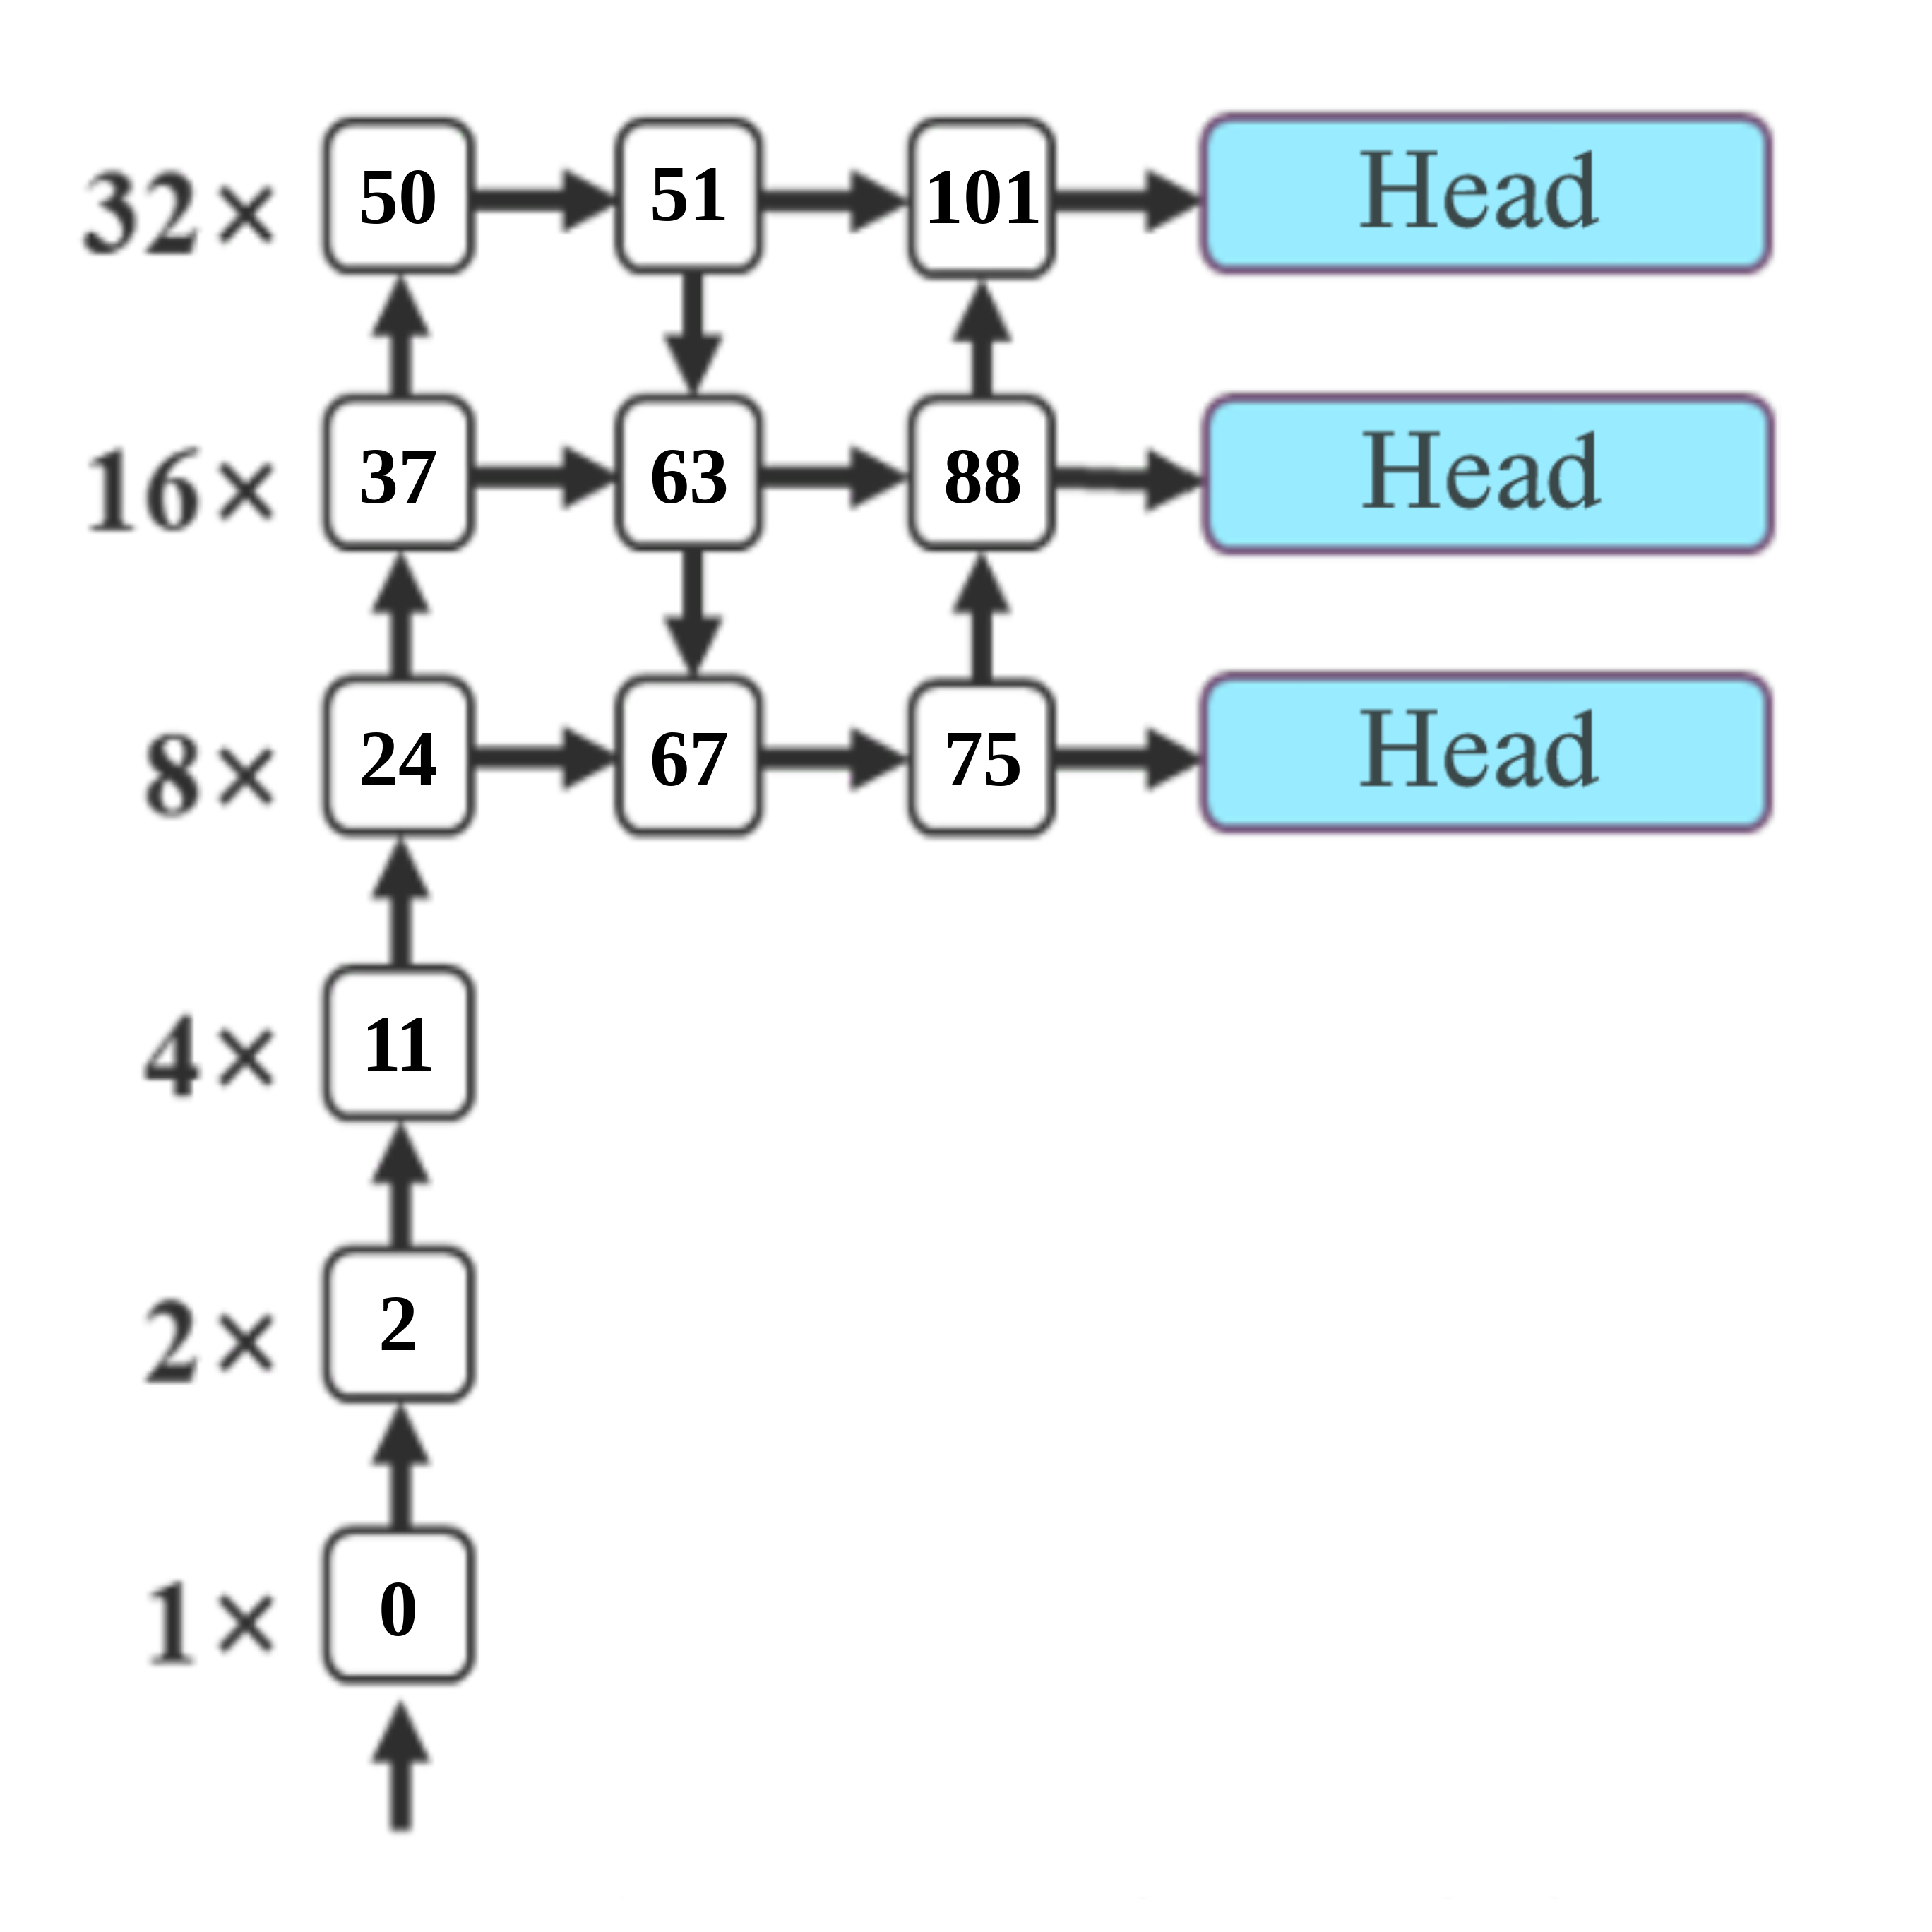
\includegraphics[width=1\linewidth]{figures/deeperconn-before.png}
      \caption{Before Rerouting}
      \label{fig:deeperconn-before}
    \end{subfigure}\hfill%\hspace{4em}
    \begin{subfigure}[][][t]{0.4\textwidth}
      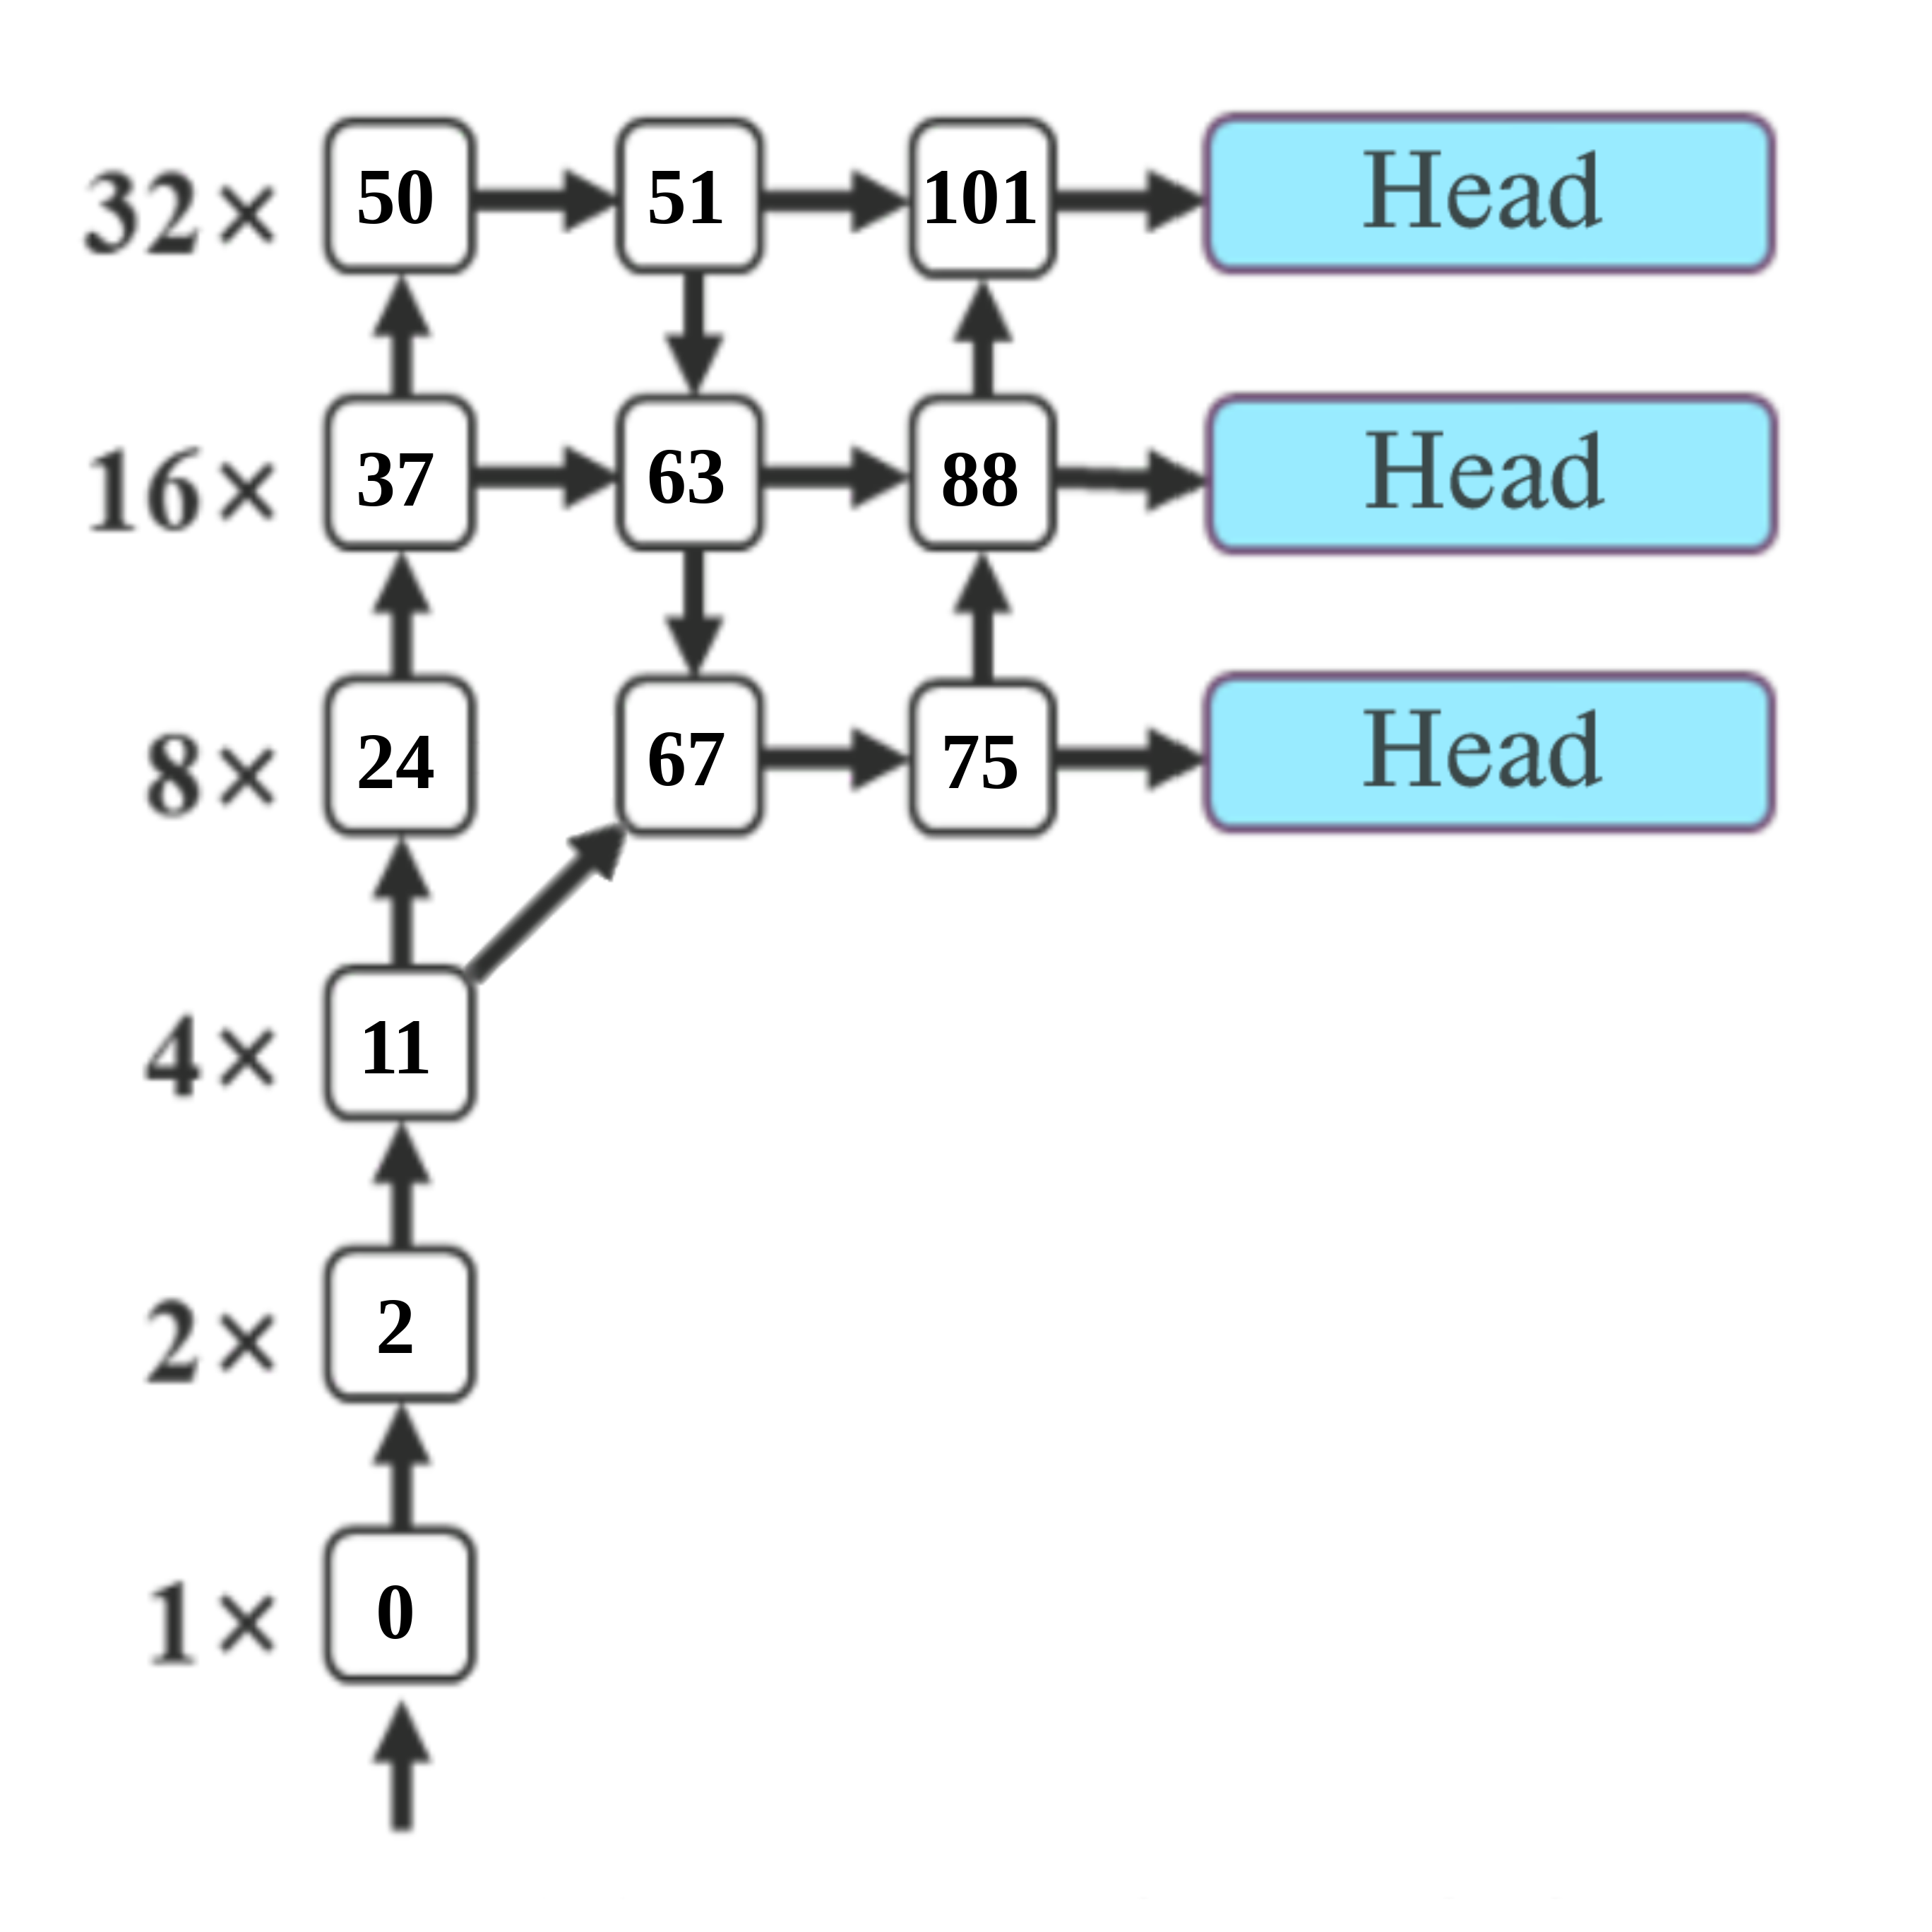
\includegraphics[width=1\linewidth]{figures/deeperconn-after.png}
      \caption{After Rerouting}
      \label{fig:deeperconn-after}
    \end{subfigure}
    \caption*{Adapted from: \textcite{yolov7} with permission (see Appendix \ref{appendix:license})}
    \caption{Modifying Connection to Earlier Feature Map Stage}
    \label{fig:deeperconn}
\end{figure}
%\begin{figure}[H]
%  \centering
%  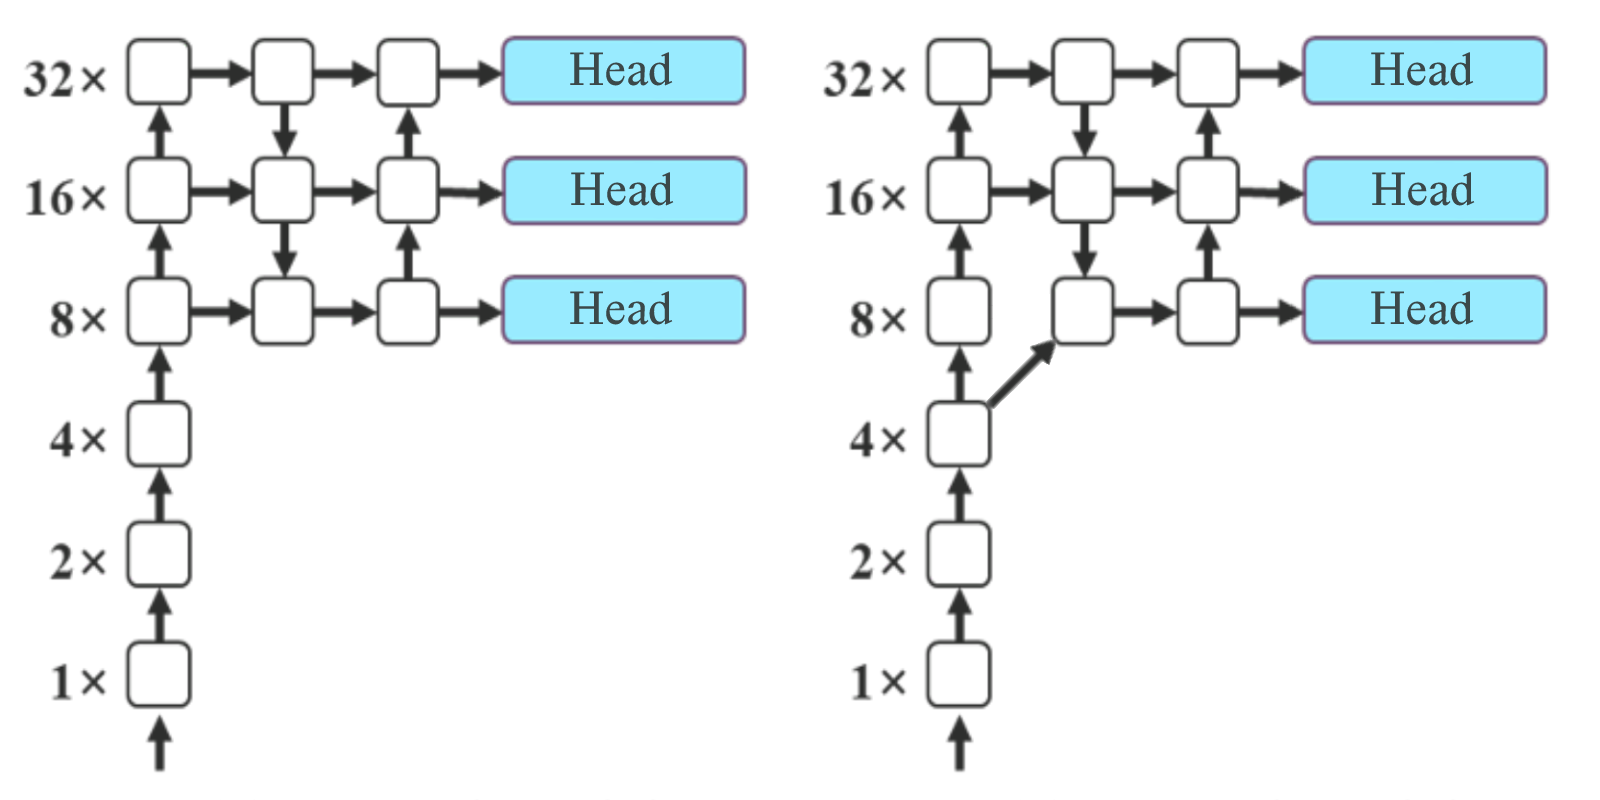
\includegraphics[width=0.7\textwidth]{figures/deeperconn.png}
%  \caption{Modifikasi Koneksi Neck. Kiri : Sebelum. Kanan : Sesudah.}
%  \label{fig:deeperconn}
%\end{figure}

As presented in Table \ref{tbl:neck_backbone_perf}, rerouting the source of 
feature map to an earlier stage produce an improvement of 2.98\% compared to \verb*|YOLOv7-MAR|.

\begin{table}
  \centering
  \captionof{table}{Performance of The Rerouted Model}
  \label{tbl:neck_backbone_perf}
  \vspace{-1ex}
    \begin{tabular}{ l l c }
    \toprule[1.5pt]
    No & Modification                                      &mAP@50 \\
    \midrule
    0  & \texttt{YOLOv7-MAR}                           & 11.2\%\\
    1  & \texttt{\textbf{YOLOv7-MAR + rerouting}} & \textbf{14.09\%}\\
    \midrule
       & Improvement                                & \textbf{\textcolor{green}{+2.98\%}}\\
    \bottomrule[1.5pt]
  \end{tabular}
\end{table}

%Perbandingan performa modifikasi ini dengan \verb*|YOLOv7-base| dapat dilihat pada tabel \ref{tbl:neck_backbone_perf}.
%Terlihat bahwa modifikasi ini berhasil meningkatkan skor mAP@50
%dari \verb*|YOLOv7-base| sebesar 2,98\%. Untuk mempermudah perbandingan dengan modifikasi lain, model hasil modifikasi
%ini akan disebut \verb*|YOLOv7-moveconnection|
\vspace{2ex}

\section{Additional YOLO Detection Head}
%Untuk modifikasi ini, pada skala 4 backbone, dipasangkan suatu layer head tambahan.
%Ilustrasi penambahan layer ini dapat dilihat pada gambar \ref{fig:addinghead}.
To add additional head layer, we utilized the feature map at the P2 scale of the network.
We introduced an upsampling block after layer 75 and fused it with layer 11 at layer 79 by concatenation.
To maintain the continuity of the network, we introduced a downsampling block that concludes at layer 87.
The subsequent layers in the network retained their original structure, but with layer numbering shifted by 25
as seen on Figure \ref{fig:addinghead}.
\begin{figure}
  \centering
  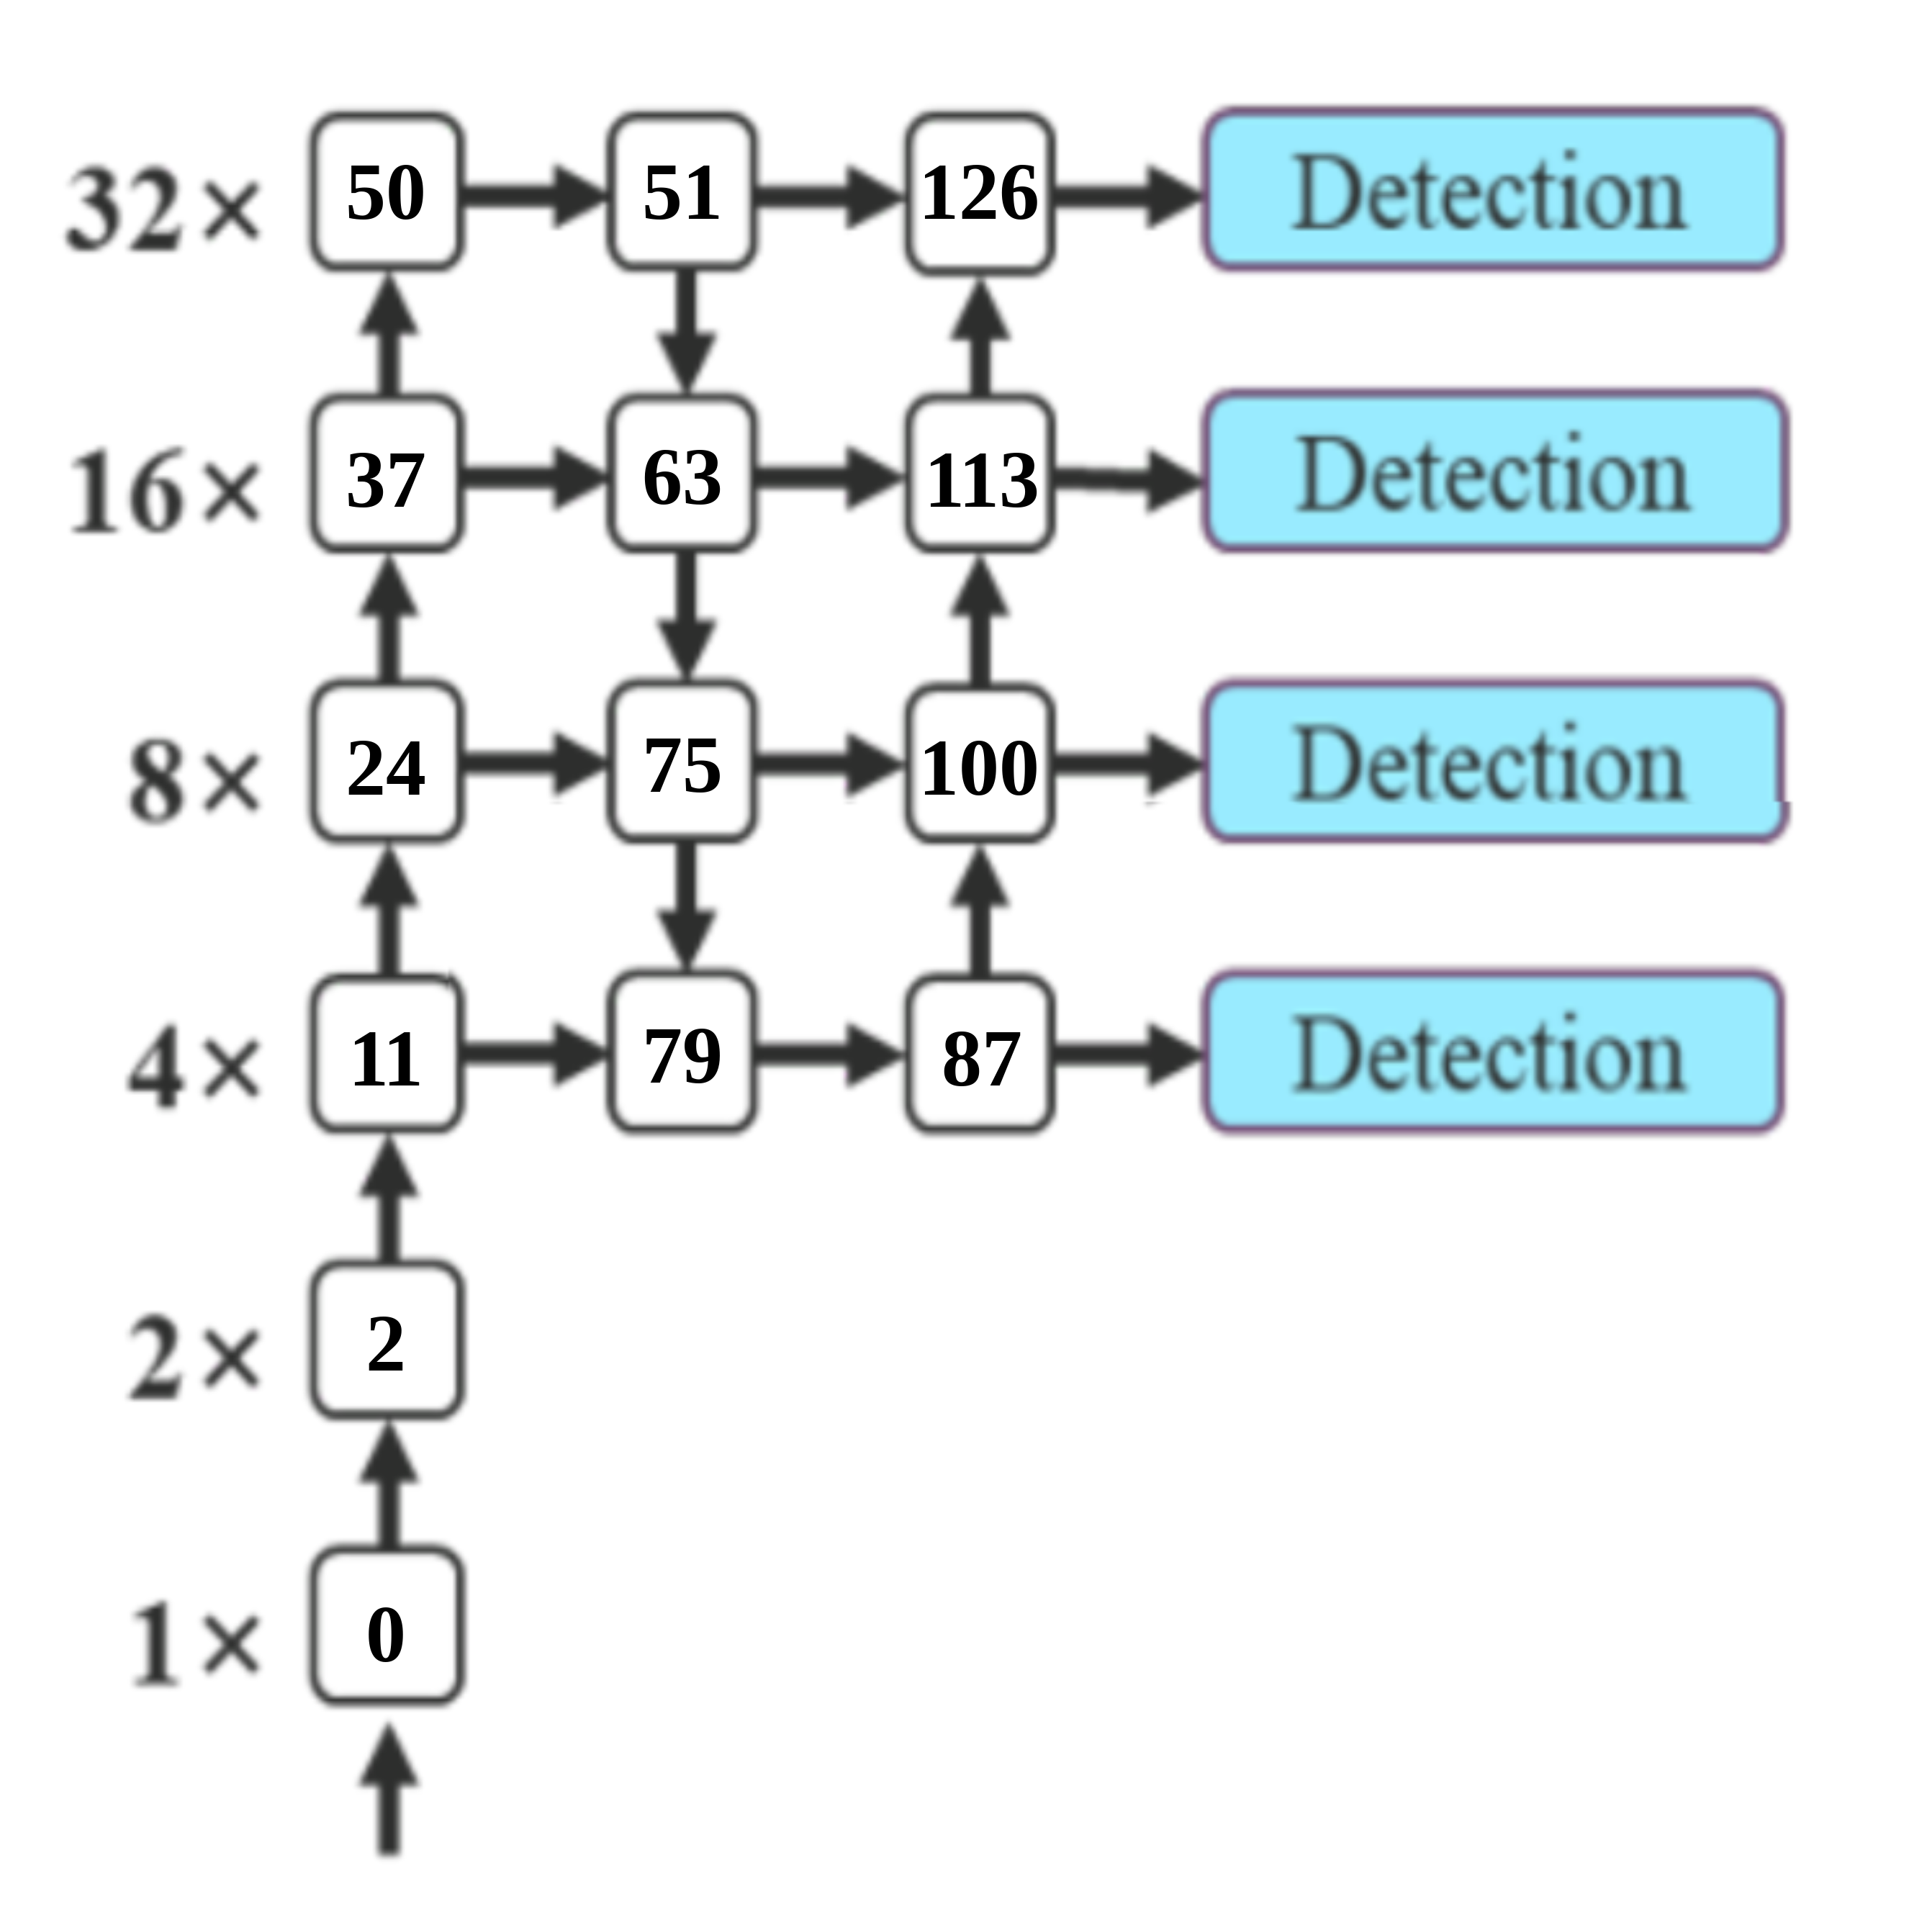
\includegraphics[width=0.35\textwidth]{figures/addheadn.png}
  \caption{Model Architecture After Increasing The Head}
  \label{fig:addinghead}
\end{figure}

\begin{table}
  \centering
  \captionof{table}{Additional Head Performance}
  \label{tbl:addhead}
  \vspace{-1ex}
    \begin{tabular}{ l l c }
    \toprule[1.5pt]
    No & Modifikasi                                 &mAP@50 \\
    \midrule
    0  & \texttt{YOLOv7-MAR}                        & \textbf{11.2\%}\\
    1  & \texttt{YOLOv7-MAR + more head}            & 5.19\%\\
    \midrule
       & Improvement                                & \textbf{\textcolor{red}{-6\%}}\\
    \bottomrule[1.5pt]
  \end{tabular}
\end{table}

As depicted in Table \ref{tbl:addhead}, additional head layer hurt the performance of the model.
This is counterintuitive. We had seen P2 feature map capable of increasing the mAP in previous section.
If we look at the loss at validation set, we can see that \verb|YOLO-MAR + head| is 
minimizing the localization loss more than \verb|YOLO-MAR + rerouting|.
There are several reasons we thought of why this happened:
\begin{enumerate}
  \item The network was simply producing loose bounding boxes prediction which looks better in loss function
  but fail when threshold criteria like in $mAP@50$ is introduced.

  \item This is an effect of bad choice of hyperparameters.
\end{enumerate}

%Seperti yang dapat dilihat pada tabel \ref{tbl:addhead}, penambahan modifikasi ini memberi performa 
%yang lebih buruk dibandingkan \verb*|YOLOv7-base|. 
%Padahal, modifikasi penambahan layer head dan \verb*|YOLOv7-moveconnection| dua-duanya menggunakan fitur pada skala 4.
%Alasan untuk hal ini akan diinvestiagsi dengan melihat output dari tiap skala pada model penambahan head dan \verb*|YOLOv7-moveconnection|.

\section{Decoupled Anchor-free Head}
%Penggantian \emph{head} menjadi \emph{decoupled anchor-free head} membuat model tidak mampu mendeteksi apapun pada dataset uji (mAP=0\%).
We experimented with replacing the coupled YOLO head to of a decoupled anchor-free head.
Upon replacing the head, we also replaced the label assigner from SimOTA to TAL.
The performance of this modification is shown in Table \ref{tbl:anchorfree_perf}.

The model was initially unable to converge due to numerical instability caused by having the objects becoming too small upon downscaling.
After stabilizing the loss function to handle these cases as shown in Appendix \ref{appendix:numerical-stabilization}, 
this modification was able to improve the mAP score by 21.78\%.

\begin{table}
  \centering
  \captionof{table}{Anchor-free Head Performance}
  \label{tbl:anchorfree_perf}
  \vspace{-1ex}
  \begin{tabular}{ l l c }
  \toprule[1.5pt]
  No & Model                                 &mAP@50 \\
  \midrule
  0  & \texttt{YOLOv7-MAR (anchor head)}        & \textbf{11.2\%}\\
  1  & \texttt{YOLOv7-MAR + anchor-free head}       & 0\% Bug Fix Data Coming Up\\
  \bottomrule[1.5pt]
\end{tabular}
\end{table}


\section{Partitioning Image}
{
\begin{figure}[p]
  \centering
  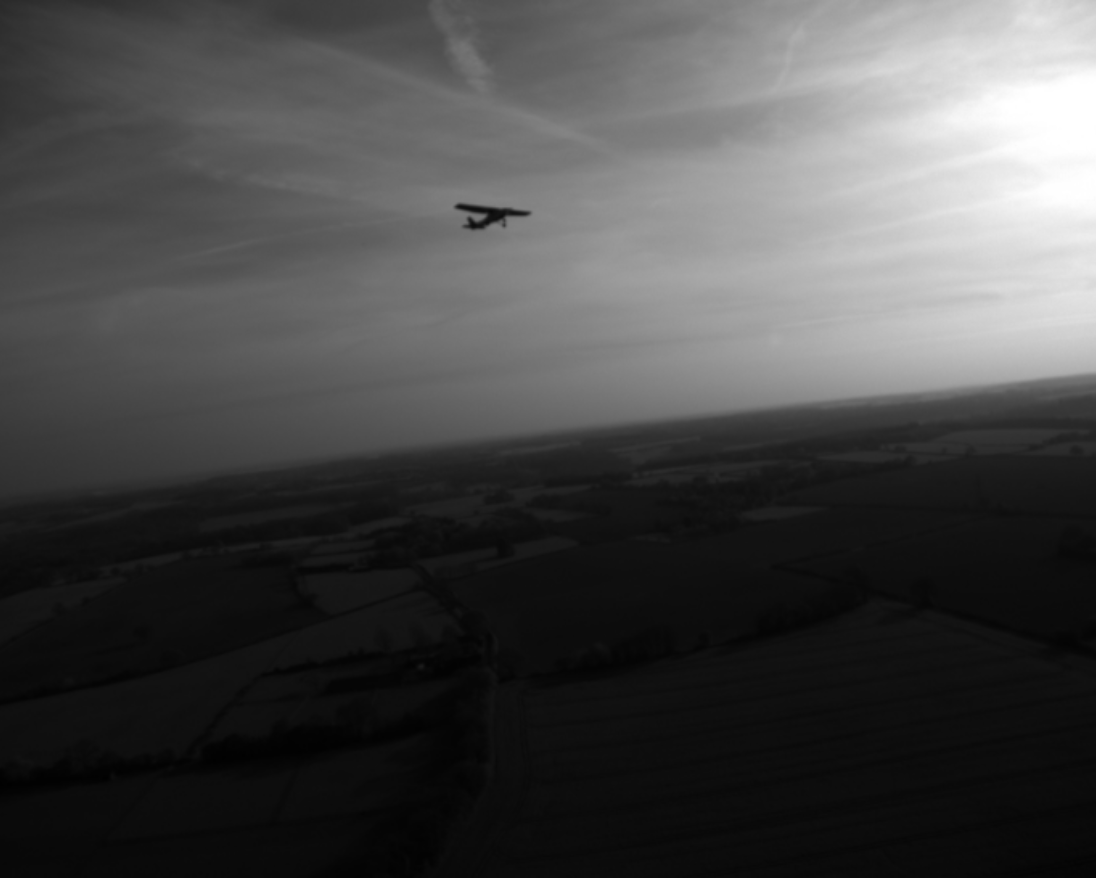
\includegraphics[height=0.33\textheight]{figures/crop_strat_source.png}
  \caption{Example Image Source for Cropping}
  \label{fig:crop-source}
\end{figure}
\begin{figure}[p]
  \centering
  \begin{subfigure}[][][t]{0.3\textwidth}
      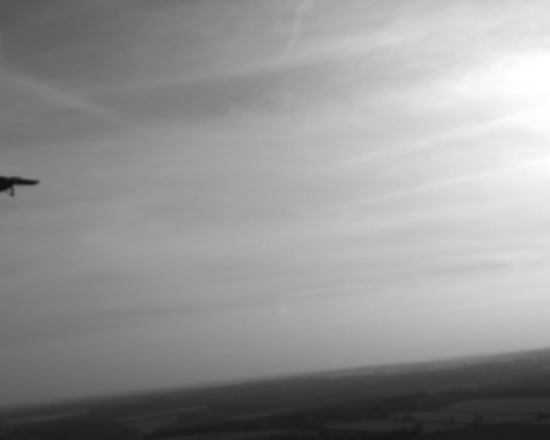
\includegraphics[width=1\linewidth]{figures/crop_strat_illegal1.png}
  \end{subfigure}
  \begin{subfigure}[][][t]{0.3\textwidth}
      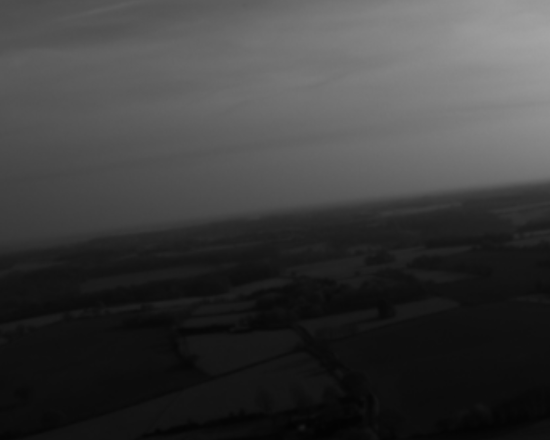
\includegraphics[width=1\linewidth]{figures/crop_strat_illegal2.png}
  \end{subfigure}
  \begin{subfigure}[][][t]{0.3\textwidth}
      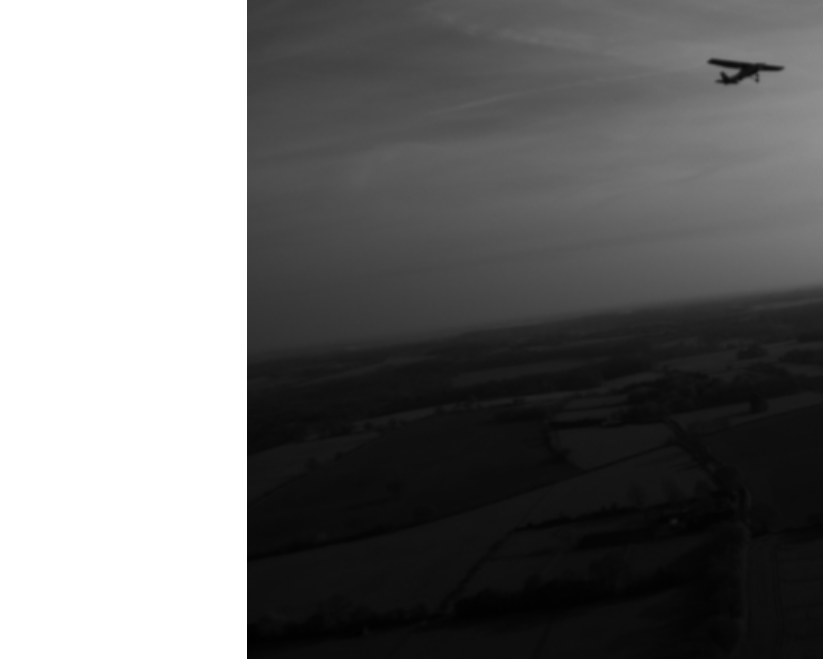
\includegraphics[width=1\linewidth]{figures/crop_strat_illegal3.png}
  \end{subfigure}
  \caption{Cropping without Strategy (Random Center)}
  \label{fig:crop-illegal}
\end{figure}
\begin{figure}[p]
  \centering
  \begin{subfigure}[][][t]{0.3\textwidth}
      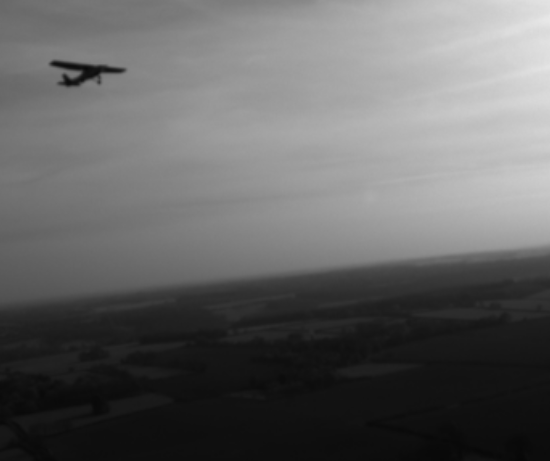
\includegraphics[width=1\linewidth]{figures/crop_strat_legal1.png}
  \end{subfigure}
  \begin{subfigure}[][][t]{0.3\textwidth}
      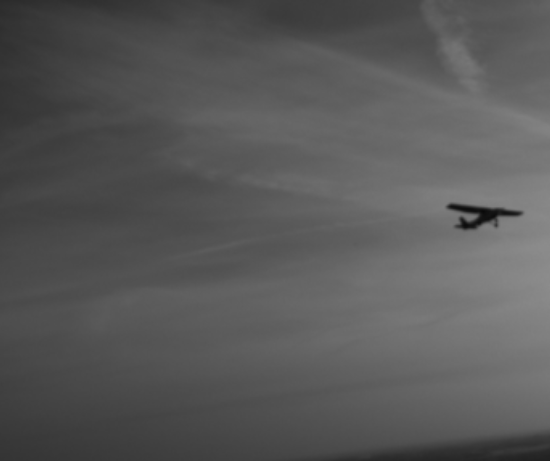
\includegraphics[width=1\linewidth]{figures/crop_strat_legal2.png}
  \end{subfigure}
  \begin{subfigure}[][][t]{0.3\textwidth}
      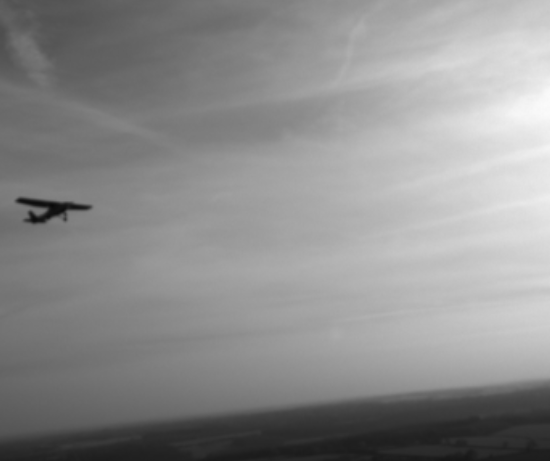
\includegraphics[width=1\linewidth]{figures/crop_strat_legal3.png}
  \end{subfigure}
  \caption{Cropping with Strategy}
  %\caption*{Cropping Strategy Guarantees the Existence of The Object}
  \label{fig:crop-legal}
\end{figure}
}
We trained the models using partitioned image of the original dataset.
In inference, we expect to partition an image into 4 equal sized images, which will
then be fed to the neural network. This way, the network will produce 4 independent
output that we can combine to form the final inference.

To generate partitioned data for training, we cropped image with size of $(W/2,H/2)$
based on the location of the objects bounding boxes. Therefore, it can be guaranteed that each image has at least
an object except for negative class images.
The procedure for this is described in the following:
\begin{itemize}[topsep=0pt]
  \item Open all images and their labels which consist of list of objects in it.
  \item For each object in an image, define a crop area with the following way:
  \begin{itemize}
    \item First, define the width and height of crop as a vector $\overrightarrow{crop_{wh}}$
    \item Then, we wanted to find a lower bound and upper bound for the x and y value that the crop center can be placed such that
    it would not cut object bounding box and not out of the boundary of the image itself. For example, for cropping the 
    image in Figure \ref{fig:crop-source}, we wanted to ensure the result would not be like in Figure \ref{fig:crop-illegal}.
    So, for the lower bound, we have:
      \begin{equation}
        \overrightarrow{crop_{lb}} = \max\left (\frac{\overrightarrow{c_{wh}}}{2} - \frac{\overrightarrow{crop_{wh}}}{2}, \frac{\overrightarrow{crop_{wh}}}{2} - \overrightarrow{c_{xy}}\right )
        \label{eq:partition-lb}
      \end{equation}
      \begin{align*}
        \text{Where}~c_{wh} &= \text{the width and height of the object's bounding box}\\
        c_{xy} &= \text{the center of the object's bounding box}\\
        \max(\vec{a},\vec{b}) &= \begin{pmatrix}\max(a.x,b.x) \\ \max(a.y,b.y)\end{pmatrix}  
      \end{align*}
    And for the upper bound:
      \begin{equation}
        \overrightarrow{crop_{ub}} = \max\left (\frac{\overrightarrow{crop_{wh}}}{2} - \frac{\overrightarrow{c_{wh}}}{2}  , 1 - \frac{\overrightarrow{crop_{wh}}}{2} - \overrightarrow{c_{xy}}\right )
        \label{eq:partition-ub}
      \end{equation}
    \item Finally, Equation \ref{eq:partition-lb} and \ref{eq:partition-ub} can be used to compute a randomized but constrained center point of the crop area
    by combining them to the following equation:
    \begin{equation}
      \overrightarrow{crop_{xy}} = \text{diag}(R)(\overrightarrow{crop_{ub}} - \overrightarrow{crop_lb}) + \overrightarrow{crop_{lb}} + \overrightarrow{c_{xy}}
    \end{equation}
    \begin{align*}
      \text{Where}~R &= \text{a random vector with value of its element is within $(0,1)$}\\
      \text{diag}(R) &= \text{a function that convert a vector $R$ to a diagonal matrix with elements of}\\ &\text{ R as its diagonal}\\
    \end{align*}
  \end{itemize}
  \item After the cropping area has been defined, the bounding boxes' values must also be converted to the cropped perspective.
  These conversions were done like the following:
  \begin{align}
    \overrightarrow{\hat{c}_{xy}} &= \overrightarrow{c_{xy}} - (\overrightarrow{crop_{xy}} - \frac{\overrightarrow{crop_{wh}}}{2})\\
    \overrightarrow{\hat{c}_{wh}} &= \frac{\overrightarrow{c_{wh}}}{\overrightarrow{crop_{wh}}} \label{eq:partition-wh-conversion}
  \end{align}
  Where the division operation in Equation \ref{eq:partition-wh-conversion} is an element-wise division, meaning the x component of the numerator is divided by the x component of the denominator, likewise for y component.
\end{itemize}
By following this procedure, it is ensured that the cropping for training image would be like in Figure \ref{fig:crop-legal} and not like Figure \ref{fig:crop-illegal}.
Without using this strategy, the resulting partitioned image for training would have a significant increase in negative class that could reduce the neural network recall ability.

The procedure so far only consider for the case when the objects are about $crop_{wh}$ away from each other.
If the objects are within $crop_{wh}$ from each other, we redefined the $c_{xy}$ and $c_{wh}$ to be the smallest box
that bounds every object in the image. Redefinition is done in the following way:
\begin{align}
  \text{Let}~B &= \text{set bounding boxes in an image} \nonumber \\
  c_{tl}.x &= \min \ \{c^*_{tl}.x : \forall\ c^* \in B\} \nonumber \\
  c_{tl}.y &= \min \ \{c^*_{tl}.y : \forall\ c^* \in B\}\nonumber \\
  c_{br}.x &= \max \ \{c^*_{br}.x : \forall\ c^* \in B\}\nonumber \\
  c_{br}.y &= \max \ \{c^*_{br}.y : \forall\ c^* \in B\}\nonumber \\
  \overrightarrow{c_{xy}} &= \frac{\overrightarrow{c_{br}}+\overrightarrow{c_{tl}}}{2} \label{eq:partition-newcxy}\\
  \overrightarrow{c_{wh}} &= \overrightarrow{c_{br}}-\overrightarrow{c_{tl}} \label{eq:partition-newcwh}
\end{align}

Since the image were partitioned to a  smaller size, we were finally able to use a smaller input size 
for the neural network. We experimented by using 640 and 960 input size on some previous modifications.
The performance is shown on Table \ref{tbl:partition-perf}.
\verb|YOLOv7-MAR + anchor-free| with input size 960 produced the greatest mAP@50 score
amongst other model when partitioned to 4.



\begin{table}[b]
  \centering
  \captionof{table}{Partitioning Image Performance}
  \label{tbl:partition-perf}
  \vspace{-1ex}
  \begin{tabular}{ l l c c c}
  \toprule[1.5pt]
  No & Model                                       &  Input Size  &Partition4 mAP@50               &mAP@50\\
  \midrule
  0  & \texttt{YOLOv7-AR}                          &     960      & 2.9\%                          &TBA\\
  1  & \texttt{YOLOv7-MAR}                         &     640      & 18.46\%                        &TBA\\
  3  & \texttt{YOLOv7-MAR}                         &     960      & 37.69\%                        &TBA\\
  4  & \texttt{YOLOv7-MAR + rerouting}             &     960      & 30.04\%                        &TBA\\
  5  & \texttt{YOLOv7-MAR + more head}             &     960      & 10.53\%                        &TBA\\
  6  & \texttt{YOLOv7-MAR + anchor-free}           &     640      & 37.57\%                        &TBA\\
  7  & \texttt{\textbf{YOLOv7-MAR + anchor-free}}  &     960      &\textbf{46.18\%}                &TBA\\
  %\midrule
  %   & Improvement                                 &              & \textbf{\textcolor{red}{-6\%}} &TBA\\
  \bottomrule[1.5pt]
\end{tabular}
\end{table}

\section{Latency}
In this section, the latency of the modifications that involved architectural changes is presented.
The data obtained using computer with specification presented in section \ref{section:instrument}.
Table \ref{tbl:inference-speed} shows that all the partition 4 models have $> 40$ FPS inference speed.
This means that they are able to perform at $>10$ FPS even without batching to detect a full image, making them all valid candidate for the best model.

As additional information, the total floating point operations (FLOPs) for each architecture modification can be seen in Table \ref{tbl:flops}.
The values are calculated using THOP profiling tool in a hardware with Fused Multiply Addition (FMA) instructions, thus it counted Multiply-Accumulate (MAC) instead of the true FLOPs.
Therefore, to find the FLOPs, output of THOP must be multiplied by 2 ($FLOPs = MAC \times 2$).
%To fin should be about
%2 times the output of THOP ($FLOPs = MAC \times 2$).

\begin{table}
  \centering
  \captionof{table}{Inference Speed of Modified Models}
  \label{tbl:inference-speed}
  \vspace{-1ex}
  \begin{adjustbox}{width=\textwidth}
  \begin{tabular}{ l l c c c}
  \toprule[1.5pt]
  No & Model                                       &   Input Size         &\multicolumn{2}{c}{Inference Speed}                   \\
     &                                             &                      &Not Reparameterized  &  Reparameterized   \\
  \midrule
  0  & \texttt{YOLOv7-MAR, plain, M, AR, EIoU}     &      1600            & 29.6 FPS            & TBA   \\
  1  & \texttt{YOLOv7-MAR + rerouting}             &      1600            & 23.28 FPS           & TBA   \\
  2  & \texttt{YOLOv7-MAR + more head}                 &      1600            & 15.91 FPS           & TBA   \\
  3  & \texttt{YOLOv7-MAR + anchor-free}               &      1600            & TBA                 & TBA   \\
  \midrule
  4  & \texttt{YOLOv7-MAR}                         &  Partition 4, 960    & TBA                 & TBA   \\
  5  & \texttt{YOLOv7-MAR + rerouting}             &  Partition 4, 960    & TBA                 & TBA   \\
  6  & \texttt{YOLOv7-MAR + more head}             &  Partition 4, 960    & TBA                 & TBA   \\
  7  & \texttt{YOLOv7-M + anchor-free}           &  Partition 4, 960    & TBA                 & TBA   \\
  \midrule
  8  & \texttt{YOLOv7-MAR}                         &  Partition 4, 640    & TBA                 & TBA   \\
  9  & \texttt{YOLOv7-MAR + rerouting}             &  Partition 4, 640    & TBA                 & TBA   \\
  10 & \texttt{YOLOv7-MAR + more head}             &  Partition 4, 640    & TBA                 & TBA   \\
  11 & \texttt{YOLOv7-M + anchor-free}           &  Partition 4, 640    & TBA                 & TBA   \\
  %\midrule
  %   & Improvement                                 &              & \textbf{\textcolor{red}{-6\%}} &TBA\\
  \bottomrule[1.5pt]
\end{tabular}
  \end{adjustbox}
\end{table}
\begin{table}
  \centering
  \captionof{table}{Floating Point Operations For a Single Inference}
  \label{tbl:flops}
  \vspace{-1ex}
  \begin{adjustbox}{width=.8\textwidth}
  \begin{tabular}{ l l c c c}
  \toprule[1.5pt]
  No & Model                                       &   Input Size         & GFLOPs (\~MAC$\times$2)         \\
  \midrule
  0  & \texttt{YOLOv7-MAR, plain, M, AR, EIoU}     &      1600            & 552.11   \\ 
  1  & \texttt{YOLOv7-MAR + rerouting}             &      1600            & 692.02   \\
  2  & \texttt{YOLOv7-MAR + more head}             &      1600            & 627.25   \\
  3  & \texttt{YOLOv7-MAR + anchor-free}           &      1600            & 1374.47  \\ 
  \midrule
  4  & \texttt{YOLOv7-MAR, plain, M, AR, EIoU}     &      960             & 205.07  \\
  5  & \texttt{YOLOv7-MAR + rerouting}             &      960             & 257.03   \\
  6  & \texttt{YOLOv7-MAR + more head}             &      960             & 232.98    \\
  7  & \texttt{YOLOv7-M + anchor-free}             &      960             & 510.53  \\
  \midrule
  8  & \texttt{YOLOv7-MAR}                         &      640             & 89.39   \\
  9  & \texttt{YOLOv7-MAR + rerouting}             &      640             & 112.04   \\
  10 & \texttt{YOLOv7-MAR + more head}             &      640             & 101.55   \\
  11 & \texttt{YOLOv7-M + anchor-free}             &      640             & 222.53   \\
  %\midrule
  %   & Improvement                                 &              & \textbf{\textcolor{red}{-6\%}} &TBA\\
  \bottomrule[1.5pt]
\end{tabular}
  \end{adjustbox}
\end{table}

\section{Model Selection}
Since all the modified models qualify for model selection as shown in Table \ref{tbl:inference-speed},
we only have to pick the model that has the largest mAP.
From Table \ref{tbl:mosaic_reanchor_performance}, \ref{tbl:loss_function_perf}, \ref{tbl:neck_backbone_perf}, \ref{tbl:addhead}, \ref{tbl:anchorfree_perf}, and \ref{tbl:partition-perf},
we found that \texttt{YOLOv7-M + anchor-free + Partition4} with input size 960 to have the largest
mAP score that is 46.18\%.

An example of detection result from this model can be seen on Figure \ref{fig:inference-out}.
As shown in the figure, the model was able to localize and classify the helicopter when it was still very far away.

\begin{figure}[btp]
  \centering
  \begin{subfigure}{\textwidth}
    \centering
    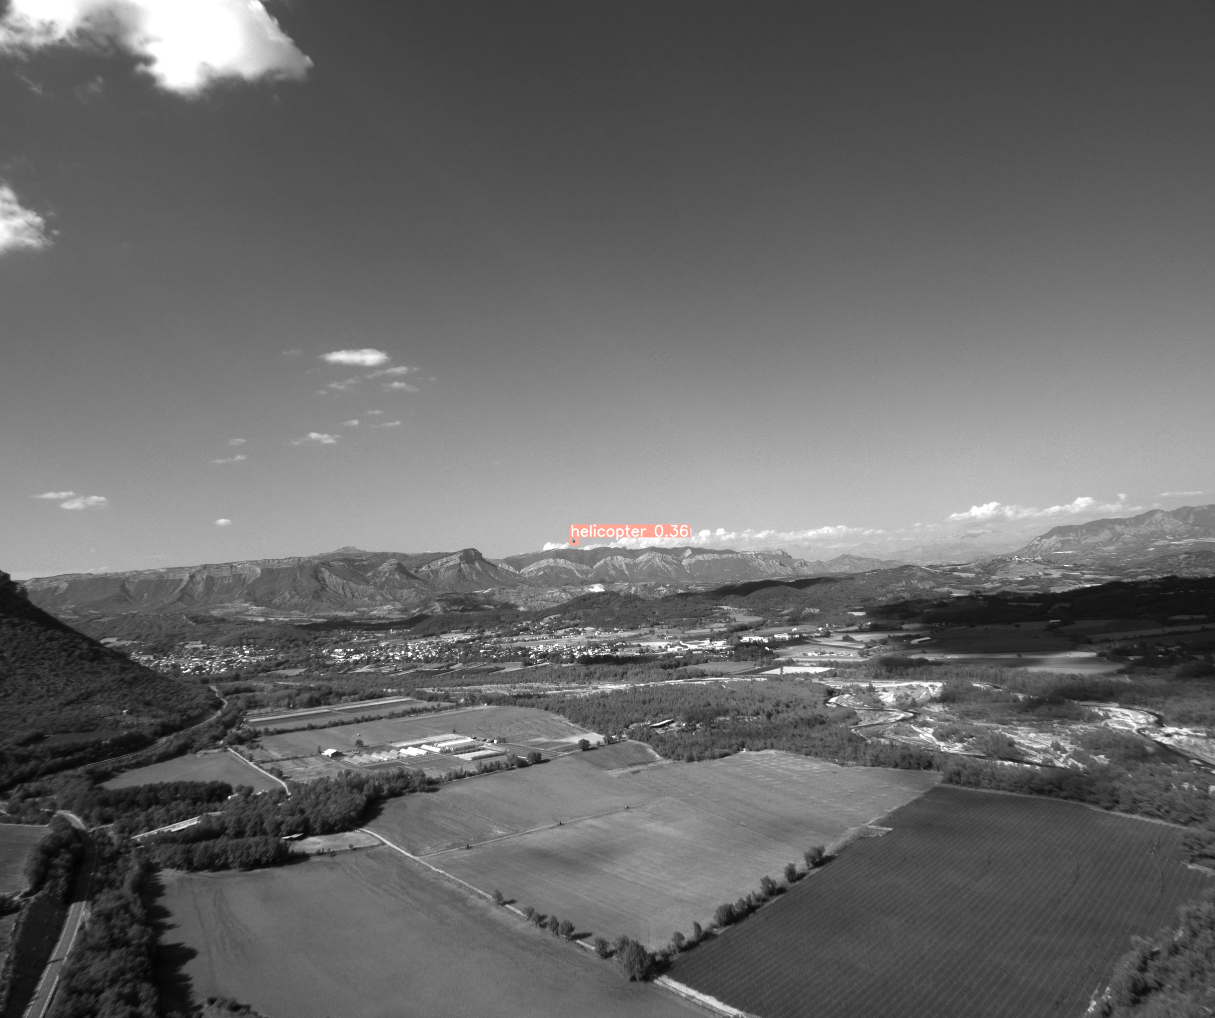
\includegraphics[width = .45\linewidth]{figures/best-1.png}
  \end{subfigure}
  \vspace{1ex}

  \begin{subfigure}{.45\textwidth}
    \centering
    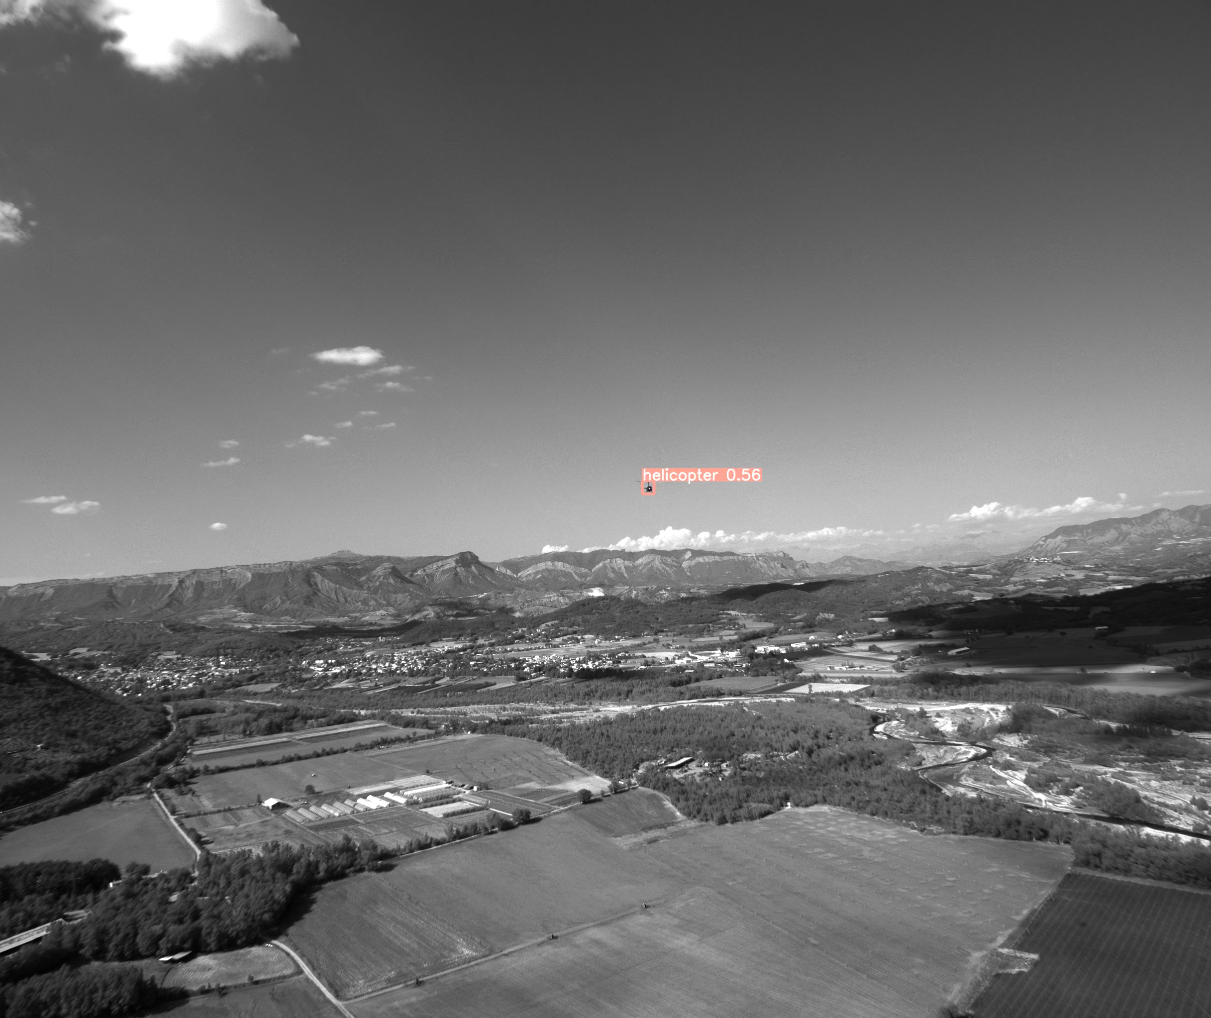
\includegraphics[width = \linewidth]{figures/best-2.png}
  \end{subfigure}\hspace{1ex}
  \begin{subfigure}{.45\textwidth}
    \centering
    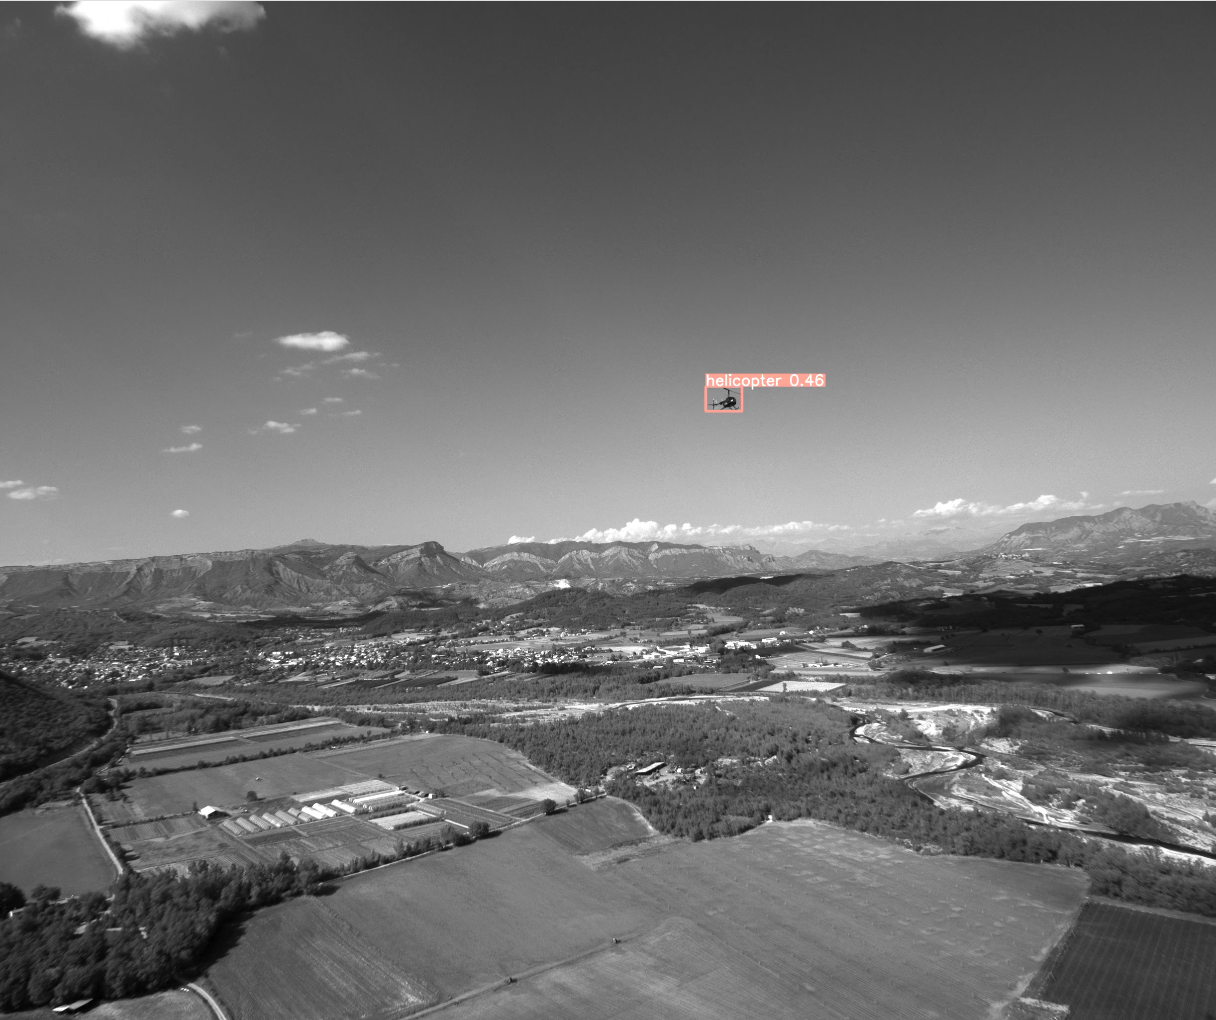
\includegraphics[width = \linewidth]{figures/best-3.png}
  \end{subfigure}
  \caption{Example Prediction Result of The Selected Best Model}
  \label{fig:inference-out}
\end{figure}
\section{Exploratory Analysis: Low Resolution/Pixel Density Images}
The dataset we used to train and benchmark so far have $2048\times 2448$ resolution.
This means that it is highly probable that the small objects are recognizable if we zoom in the image.
But what about objects that are not recognizable even after zooming?
In this section, we would like to experiment with low resolution or low pixel density input.
The purpose of this experiment is to find out the performance of the selected best modified YOLOv7 models against
bad quality image. We want to find out its ability to predict vague looking objects.

For the experiment, we purposely select some images from \textcite{mva2023} that has hard to recognize airborne objects in it, even after zooming.
These images will first converted into grayscale to make it similar with the training dataset that was obtained from \textcite{aot_dataset}.
\textcite{mva2023} images quality are different compared to \textcite{aot_dataset}.
Although it has higher pixel resolution, \textcite{mva2023} images' pixel density is subpar compared to \textcite{aot_dataset}.
Observe Figure \ref{fig:mva}, the object is almost not recognizable even after zooming due to low pixel density, different from Figure \ref{fig:airborne-object-example-1} introduced in section \ref{section:background}.

After running these low pixel density images with the best modified YOLOv7 model, we found that the model was unable to correctly detect the airborne objects in them.
The model did not detect any airborne objects on most images. On some rare cases, the model was able to localize the airborne object but unable to classify it to the proper class.
One example for such cases is the image in Figure \ref{fig:mva}. The model was able to localize the birds properly, but classify them as airplane.
We also tried to crop the images so that it would have the same resolution as \textcite{aot_dataset}, but the result remain the same.

This experiment is an evidence that the model was unable to perform inference on low detail quality image.
However, this outcome might be caused by the training data significantly different to \textcite{mva2023} rather than the fault of the model itself.
The model was trained on dataset where all the images was taken from the same or similar camera that produce high pixel density images.
It is possible that inclusion of bad quality image in the dataset would improve the model ability to perform detection on low pixel density images.

\begin{figure}[btp]
  \centering
  \includegraphics[height=0.6\textwidth]{figures/mva.png}
  \caption*{Source: \textcite{mva2023}, permissible under copyright license (see Appendix \ref{appendix:license})}
  \caption{Example Low Pixel Density Image in \textcite{mva2023}}
  \label{fig:mva}
\end{figure}

\cleardoublepage

% contents 5 penutup
\chapter{CONCLUSION}

% Ubah bagian-bagian berikut dengan isi dari penutup

\section{Conclusion}
\label{section:conclusion}

Based on the experiments conducted in previous chapter, it can be observed that some specific modification
can improve YOLOv7 ability on detecting airborne objects, while others have negligible or even negative effect.
In conclusion, we found that:
\begin{itemize}[noitemsep,topsep=0pt]
  \item YOLOv7 was only able to perform detection on airborne objects after adding mosaic augmentation to the training data and recalculated its anchor to fit the data.
  This modification improved the mAP score from 0 to 11.2\%.
  \item EIoU, even with its convexication technique, was not able to outperform YOLOv7's original CIoU. It produced only 4.92\% in mAP score.
  \item Rerouting the detection to use an earlier stage of feature map can improve slightly improve the mAP.
  \item Additional head on YOLOv7 did not perform better than original 3 head.
  \item Replacing head to a decoupled anchor free head greatly improve the detection capability.
  \item Applying image partition to all model greatly improve their detection performance. The greatest performance after applying image partition
  came from anchor-free head modification which produced 46.18\% mAP, a 13.2\% improvement compared to without partition.
\end{itemize}
Amongst all the proposed modifications applied to YOLOv7, we also found that applying image partition, and replacing
head to a decoupled anchor free head performed the best on detecting airborne objects, while still able to perform inference in real-time.


With this, we have explored different ways to improve the detection of airborne objects with YOLOv7.
However, there are still more things we can try in the future to make it even better.
One idea is to use attention mechanisms, which help the model focus on important features related to airborne objects.
We could also investigate transfer learning and domain adaptation to leverage existing knowledge and adapt the model to specific situations.
To handle low pixel density data, we could introduce subpixel convolutions instead of pyramid upsampling when increasing the dimension of features.
Overall, there are still many opportunities for further research and enhancements that could be done in optimizing YOLOv7 airborne object detection.
%\section{Discussion}

%Based on the experiments conducted in previous chapter, we can conclude that:
%among the modification candidates proposed in this research, we found the combination
%of mosaic augmentation, anchor recalculation, and rerouting feature map from P3 to P2
%produced the greatest mAP@50 score 14.09\%. 
%Another improvement we made by partitioning in the input image and perform inference 
%on each of them independently. We find that a YOLOv7 model with mosaic augmentation,
%and replacement of head layer with decoupled anchor-free head gives out the greatest
%mAP@50 score of 46.18\%. 
%Berdasarkan hasil pengujian yang dilakukan, dapat disimpulkan bahwa:
%Dari himpunan modifikasi-modifikasi yang diajukan pada penelitian ini,
%didapatkan kombinasi modifikasi yang paling optimal.
%Modifikasi tersebut penambahan augmentasi mosaik, rekalkulasi anchor, dan pemindahan koneksi neck-backbone.
%Dengan modifikasi itu, skor mAP@50 dari YOLOv7 meningkat sebanyak 14,09\%.

%\section{Discussion}
%Modifikasi-modifikasi yang diaplikasikan pada penelitian ini hingga saat ini
%masih dibatasi pada modifikasi yang tidak secara signifikan mempengaruhi \emph{latency}.
%Beberapa modifikasi seperti melakukan partisi pada gambar, dan melakukan deteksi di
%tiap partisinya. Dengan metode ini, objek yang dipelajari akan terlihat lebih besar
%sehingga lebih mudah untuk dideteksi. Akan tetapi, latency pendeteksian untuk tiap gambar
%akan meningkat sebanyak jumlah partisi kali lipat. Untuk mengatasi hal tersebut,
%kita dapat melakukan down-scaling pada model yang digunakan. Modifikasi jenis ini
%perlu dicoba untuk menentukan jumlah partisi dan down-scaling model yang tepat
%untuk mempertahankan kecepatan deteksi yang \emph{real-time}.
%\section{Discussion}
%With greater computaational resource, this research could probably be better.




\cleardoublepage

\chapter*{DAFTAR PUSTAKA}
\addcontentsline{toc}{chapter}{DAFTAR PUSTAKA}
\renewcommand\refname{}
\vspace{2ex}
\renewcommand{\bibname}{}
\begingroup
\def\chapter*#1{}
\printbibliography
\endgroup
\cleardoublepage

% Biografi penulis
%\begin{center}
  \Large
  \textbf{BIOGRAFI PENULIS}
\end{center}

\addcontentsline{toc}{chapter}{BIOGRAFI PENULIS}

\vspace{2ex}

\begin{wrapfigure}{L}{0.3\textwidth}
  \centering
  \vspace{-3ex}
  % Ubah file gambar berikut dengan file foto dari mahasiswa
  
\includegraphics[width=0.3\textwidth]{figures/elon.jpg}
  \vspace{-4ex}
\end{wrapfigure}

% Ubah kalimat berikut dengan biografi dari mahasiswa
\name{}, lahir pada \lipsum[1]

\lipsum[2]

%\cleardoublepage

\end{document}
